\chapter{User Manual}

\section{Introduction}

\subsection{Purpose}

The purpose of the system is to easily manage the stock of the products sold at a Veterinary Center. The system achieves this purpose with the following features:

\begin{itemize}
\item{Automatically updating the stock of the products when they are purchased by a customer}
\item{Informing the user when stock needs to be moved from one location to another}
\item{informing the user that they need to buy more stock for specific products when the total stock is low.}
\end{itemize}

\subsection{Intended Audience}

The intended audience for my system is Beacon Veterinary Center. However, with minor changes to the system, such as the logo and the information stored about the product, the system could potentially be used by any company that sells products. 

\section{Installation}

\subsection{Prerequisite Installation}

%include as many subsubsections as necessary for each piece of required software

\subsubsection{Installing Python}

\subsubsection{Installing PyQt}

\subsubsection{Etc.}

\subsection{System Installation}

\subsection{Running the System}



\section{Tutorial}

\subsection{Introduction}
The following section explains how to use each component of the system. Each subsection of the tutorial gives a detailed explanation including annotated diagrams to assist you in running the system.


\subsection{Assumptions}

The Tutorial has been created under the assumption that the users will have a variety of different computer knowledge. Therefore, the tutorial has been created such that, minimal computer knowledge is required to understand it. Another assumption made, is that the system has been installed successfully, and that the system is already running. The installation tutorial can be found on page: section: and the tutorial on running the system can be found on page: section: 

\subsection{Tutorial Questions}
The following sections are a step by step guide for each section of the system. The different sections of the tutorial have been broken down into Questions which can be referenced in the contents table below:

\pagebreak
\subsubsection{Contents}

\begin{center}
    \begin{longtable}{|p{3cm}|p{6cm}|p{3cm}|}
        \hline
	 \textbf{Section Number} & \textbf{Question} & \textbf{Page Number} \\ \hline
	&How do I log in to the system? & \\ \hline
	&What should i do if i forget my user-name or password?& \\ \hline
	& What should i do if i can no longer access the email address associated with my account? & \\ \hline
	&How do i add a product to the system? & \\ \hline
	&How do i edit a product that is currently in the system?& \\ \hline
	&How do i remove a product from the system?& \\ \hline
	&How do i find a Product in the system?& \\ \hline
	&How do i change the stock of a product?& \\ \hline
	&How do i view the predicted sales of a product?& \\ \hline
	&How do i add a Member to the system?& \\ \hline
	&How do i find a Member in the system?& \\ \hline
	&How do i edit the information about a Member?& \\ \hline
	&How do i remove a Member from the system?& \\ \hline
	&How do i add an Employee to the system?& \\ \hline
	&How do i edit the information about an Employee in the system?& \\ \hline
	&How do i remove an employee from the system?& \\ \hline
	&How do i find an Employee in the system?& \\ \hline
	&How do i get to the Order interface?& \\ \hline
	&How do i add products to an order?& \\ \hline
	&How do i give a discount on the order? & \\ \hline
	&How to i preview an order once its finished?& \\ \hline
	&How do i print off an invoice?& \\ \hline
	&How do send an invoice to an email?& \\ \hline
	&How do i change the company information on the invoice? & \\ \hline
	&How do i change the company logo on the invoice?& \\ \hline
	&Why won't emails send successfully?& \\ \hline
	&How do i change my password?& \\ \hline
	&How do i access the search window?& \\ \hline
	&How do i log off the system?& \\ \hline
	\end{longtable}
\end{center}

\pagebreak

\subsubsection{Logging into the system}
\label{fig:Logging into the system}

\textbf{1.} Run the system, you will presented with the log in interface.
 
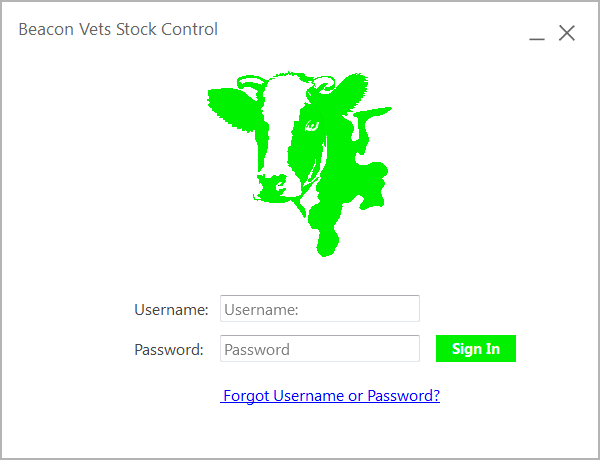
\includegraphics[width=8cm]{./ManualImages/log-in-1.png}
  
For instructions on how to run the system, go to page .

\textbf{2.} Enter your user-name into the user-name field.

\textbf{3.} Enter your password into the password field.

If you cannot remember your user-name or password, go to page .

\textbf{4.} Click the sign in button, if your log in details are correct you will be taken to the Current Order screen.

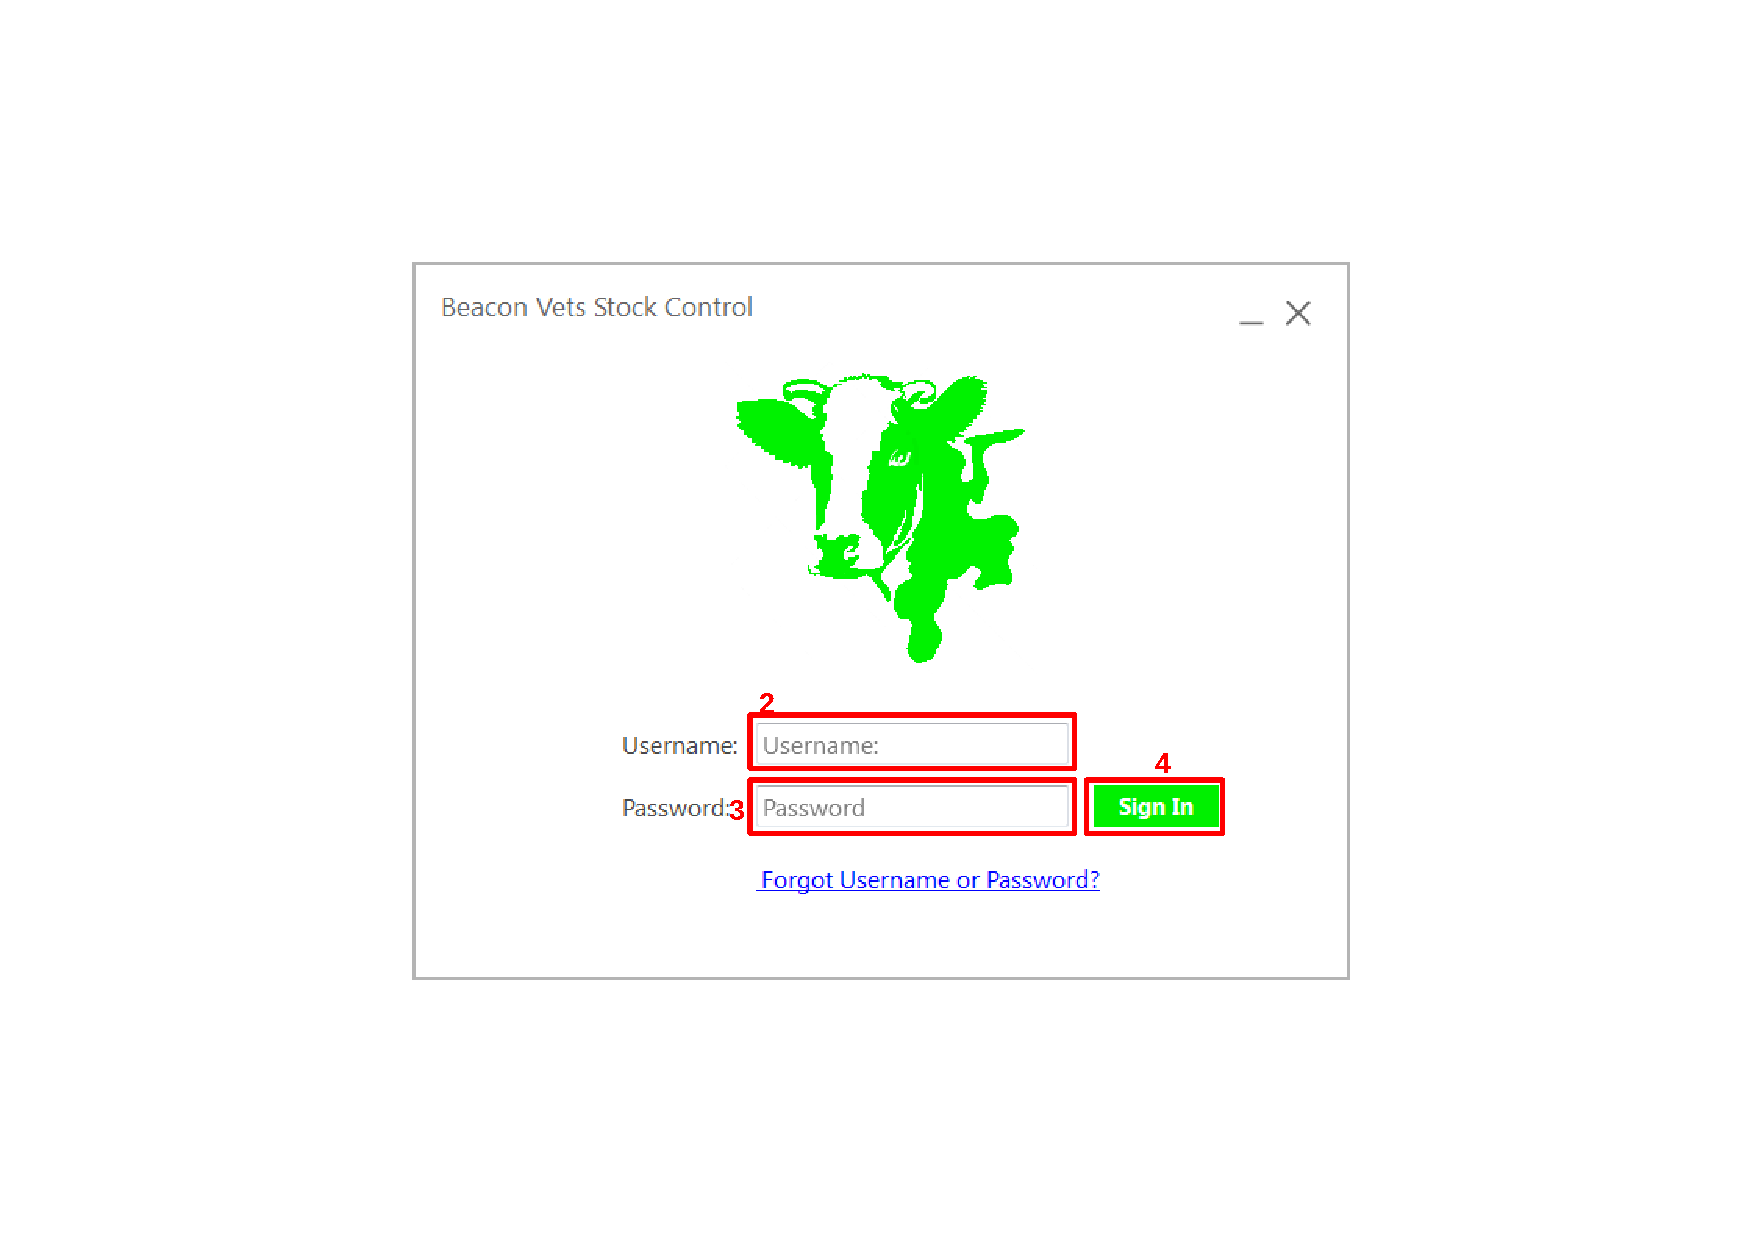
\includegraphics[width=8cm]{./ManualImages/log-in-2.pdf}

\pagebreak
\subsubsection{Logging out of the system}
\label{fig:Logging out of the system}

In order to log out of the system, you must already be logged into the system. For instructions on how to log into the system, go to page \pageref{fig:Logging into the system}.

\textbf{1.}  On any interface, Click on the `Options' button in the menu bar at the top of the page.

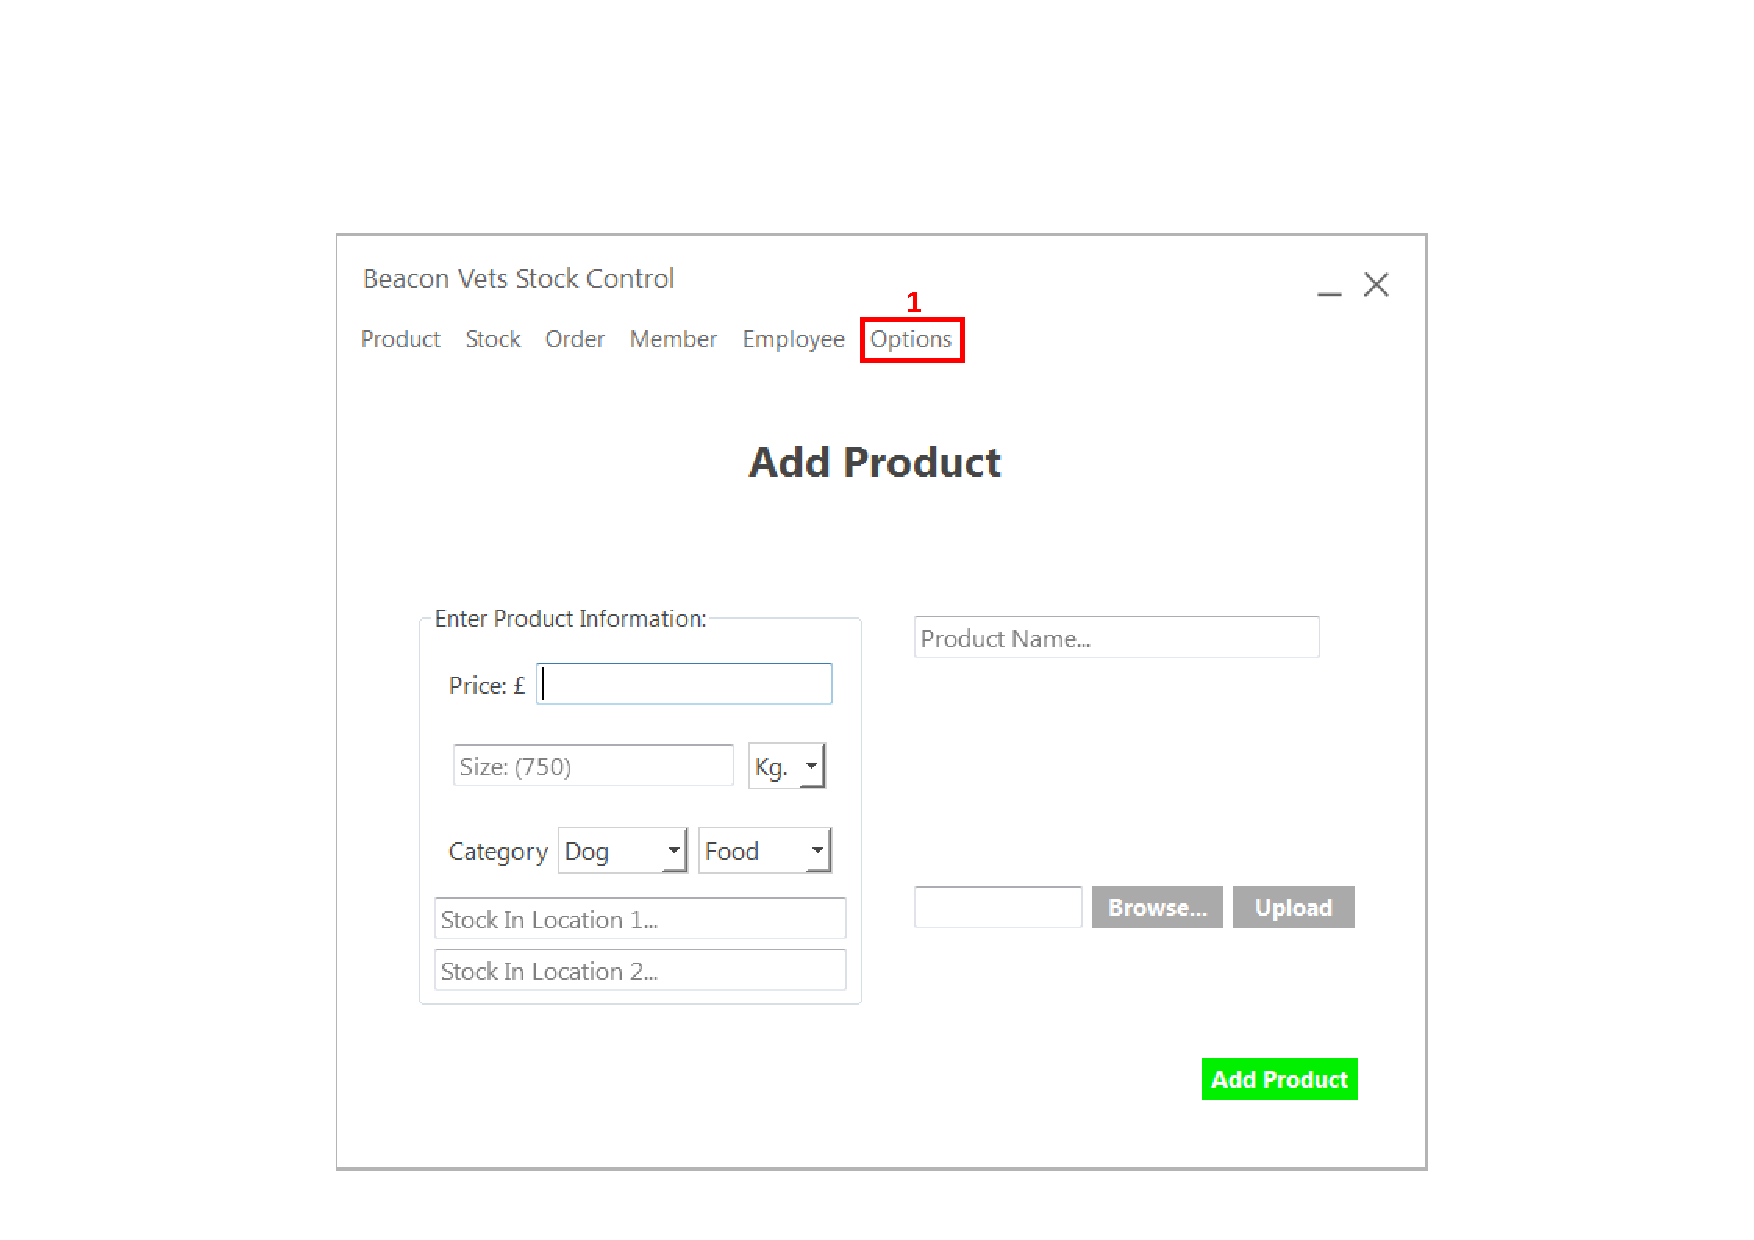
\includegraphics[width=8cm]{./ManualImages/log-off-1.pdf}

\textbf{2.} Clicking on the `Options' button will display a drop down menu. Click on the `Log Off' option from this menu.

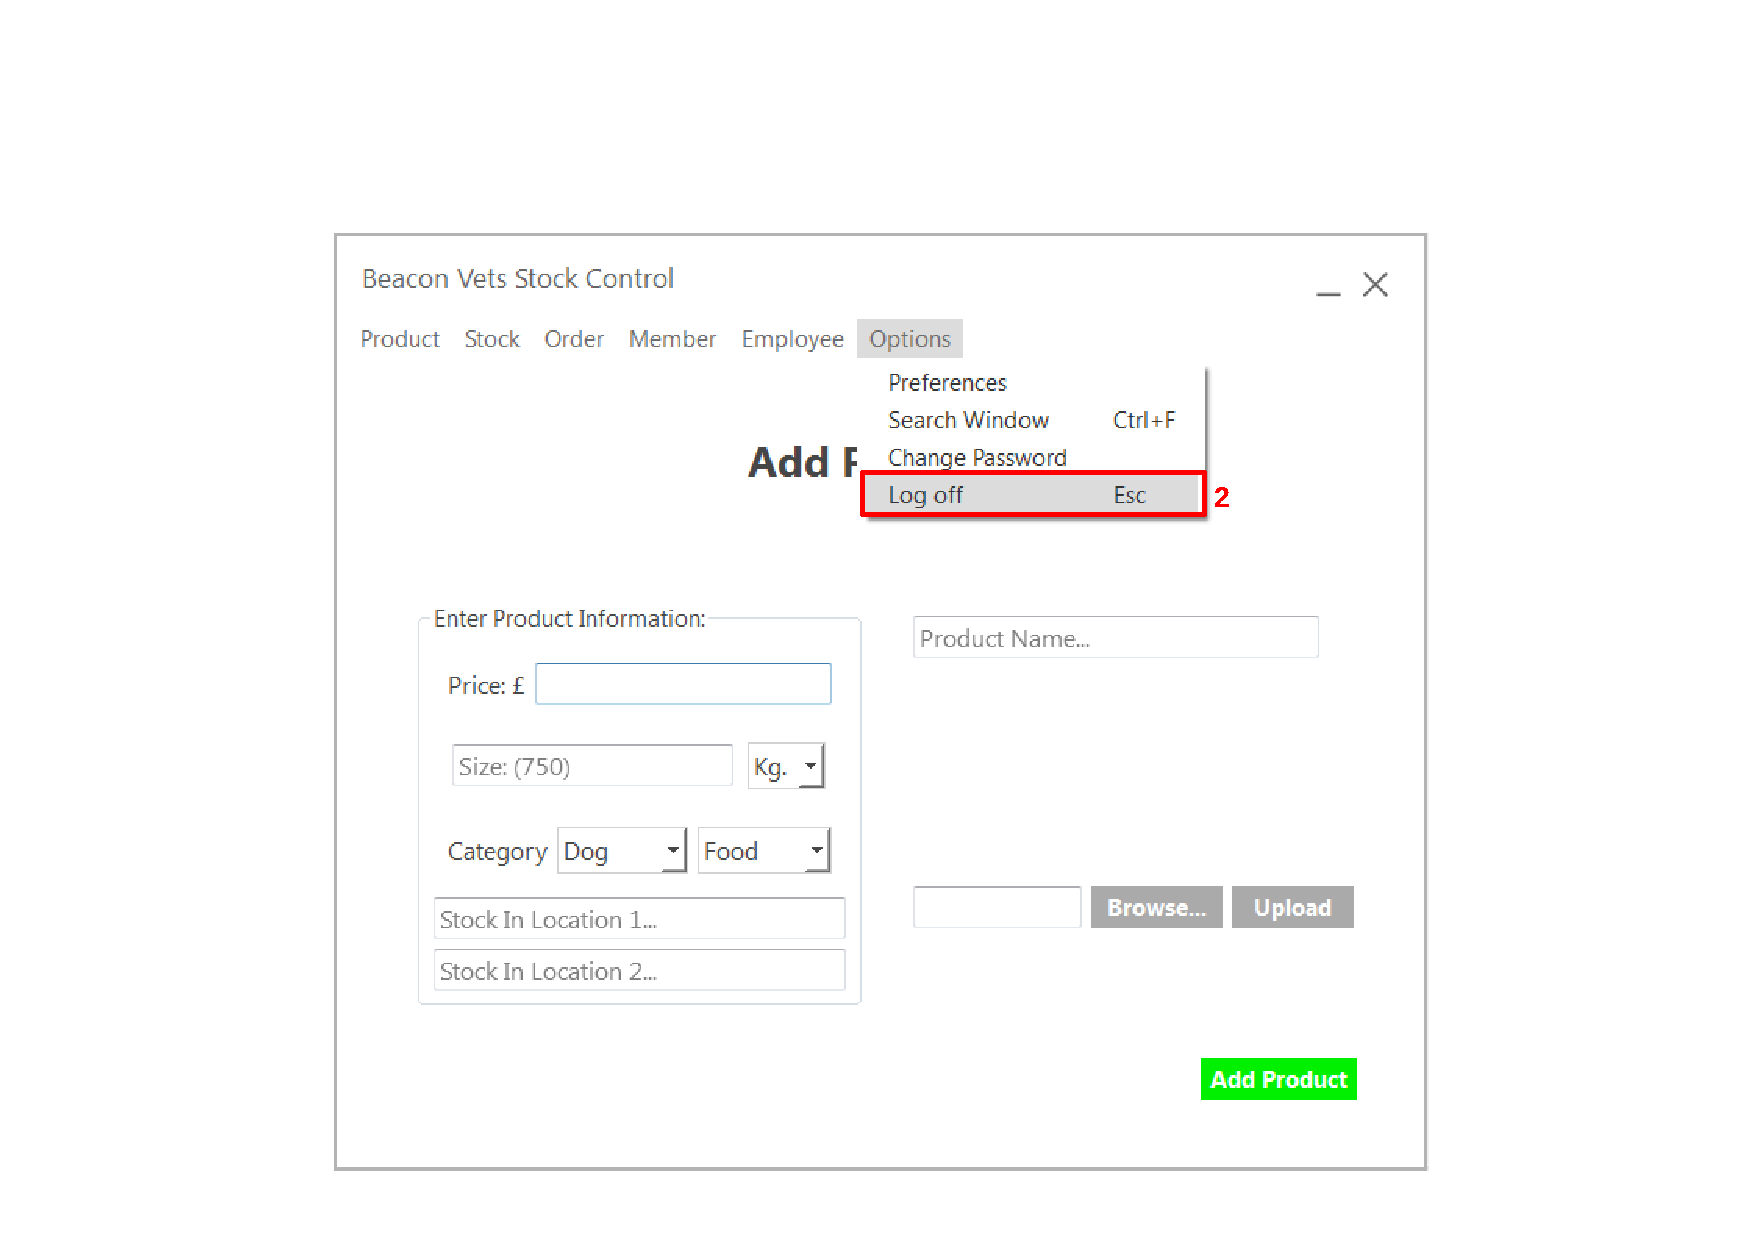
\includegraphics[width=8cm]{./ManualImages/log-off-2.pdf}

An alternative to Step 1 and Step 2 is that you can press the `ESC' button on the keyboard whilst on any interface.

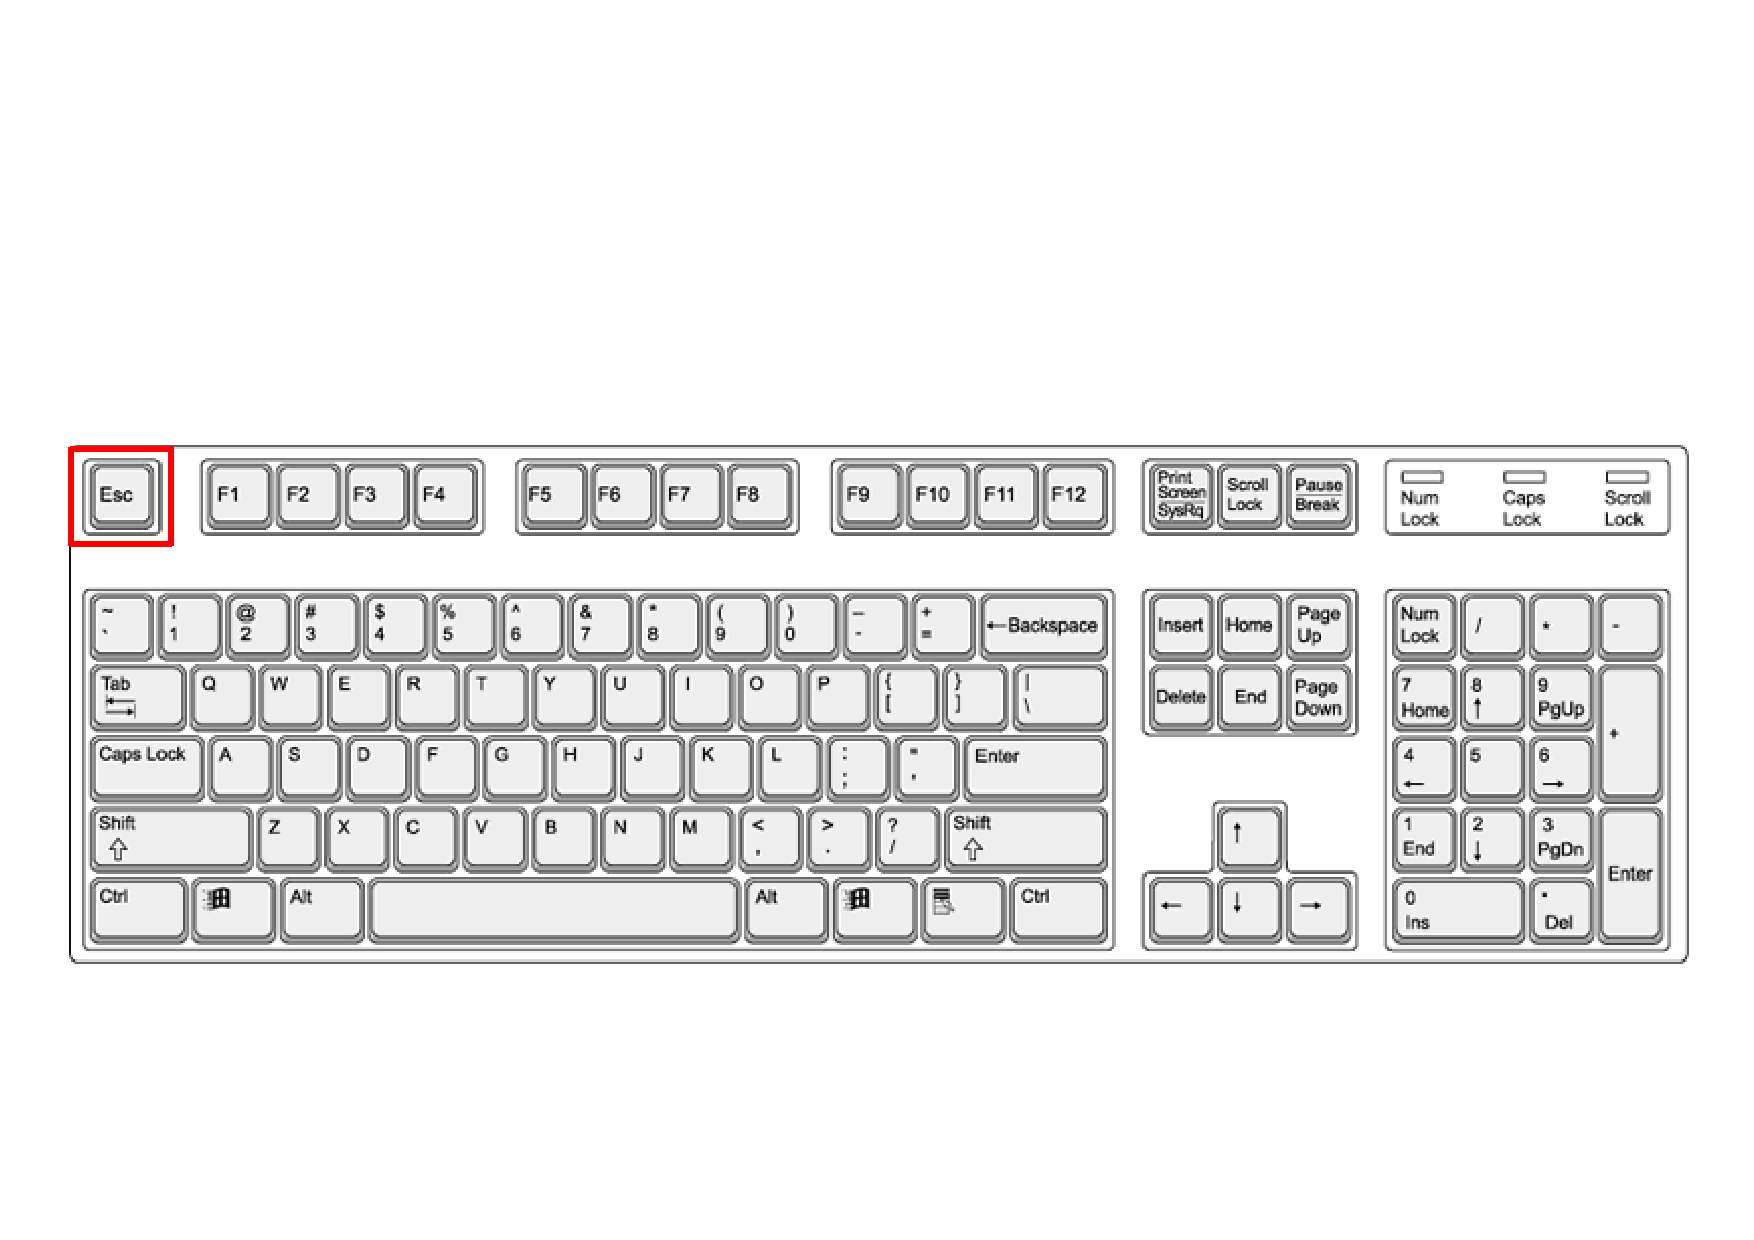
\includegraphics[width=\textwidth]{./ManualImages/shortcut-esc.pdf}

\textbf{3.} A Confirmation window will display. Click the `Yes' button.

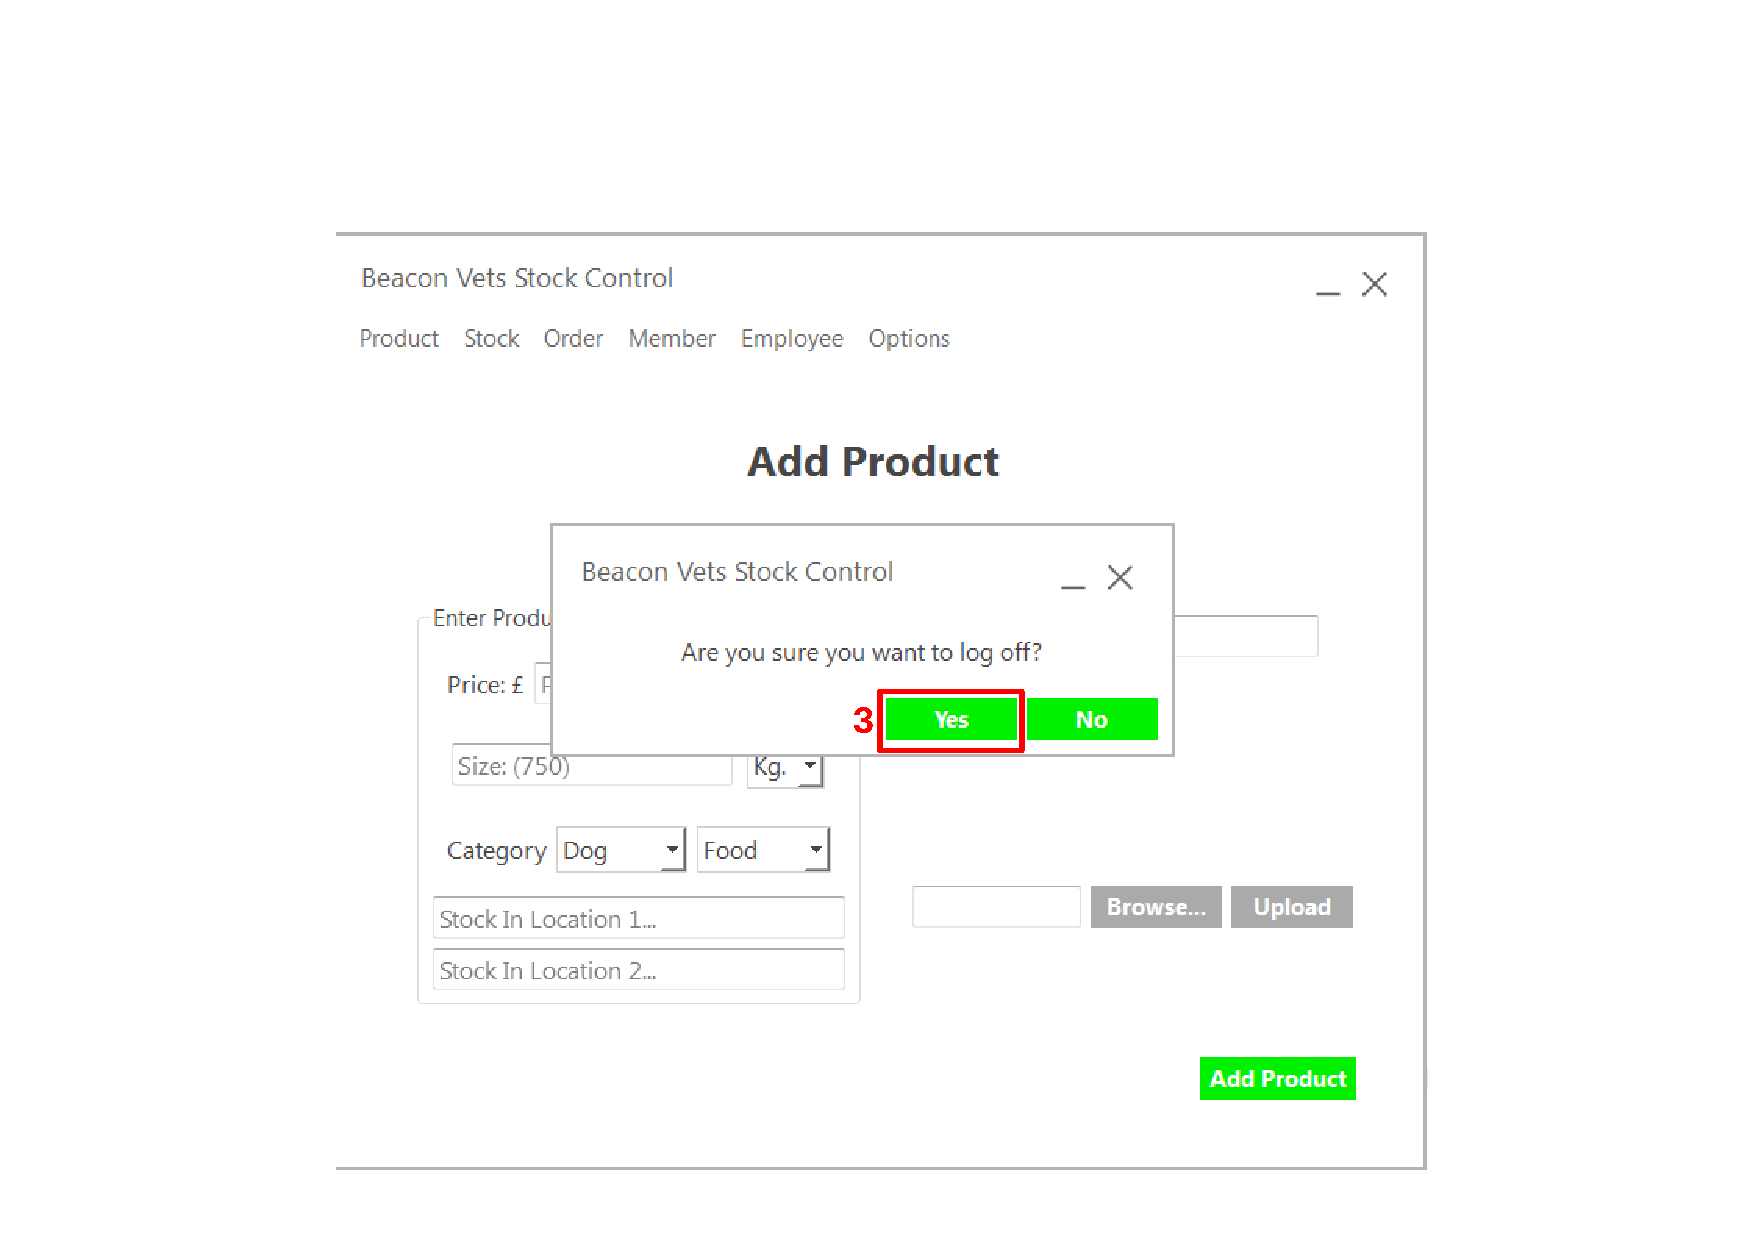
\includegraphics[width=8cm]{./ManualImages/log-off-3.pdf}

You have now logged off the system.

\pagebreak
\subsubsection{Forgetting Your User-name or Password}
\label{fig:Forgetting Your User-name or Password}

\textbf{1.} Go to the log in interface.

If you are currently logged in and do not know how to log out, go to page \pageref{fig:Logging out of the system}  for a tutorial on logging out.

\textbf{2.} Click on the `Forgot User-name or Password?' text.

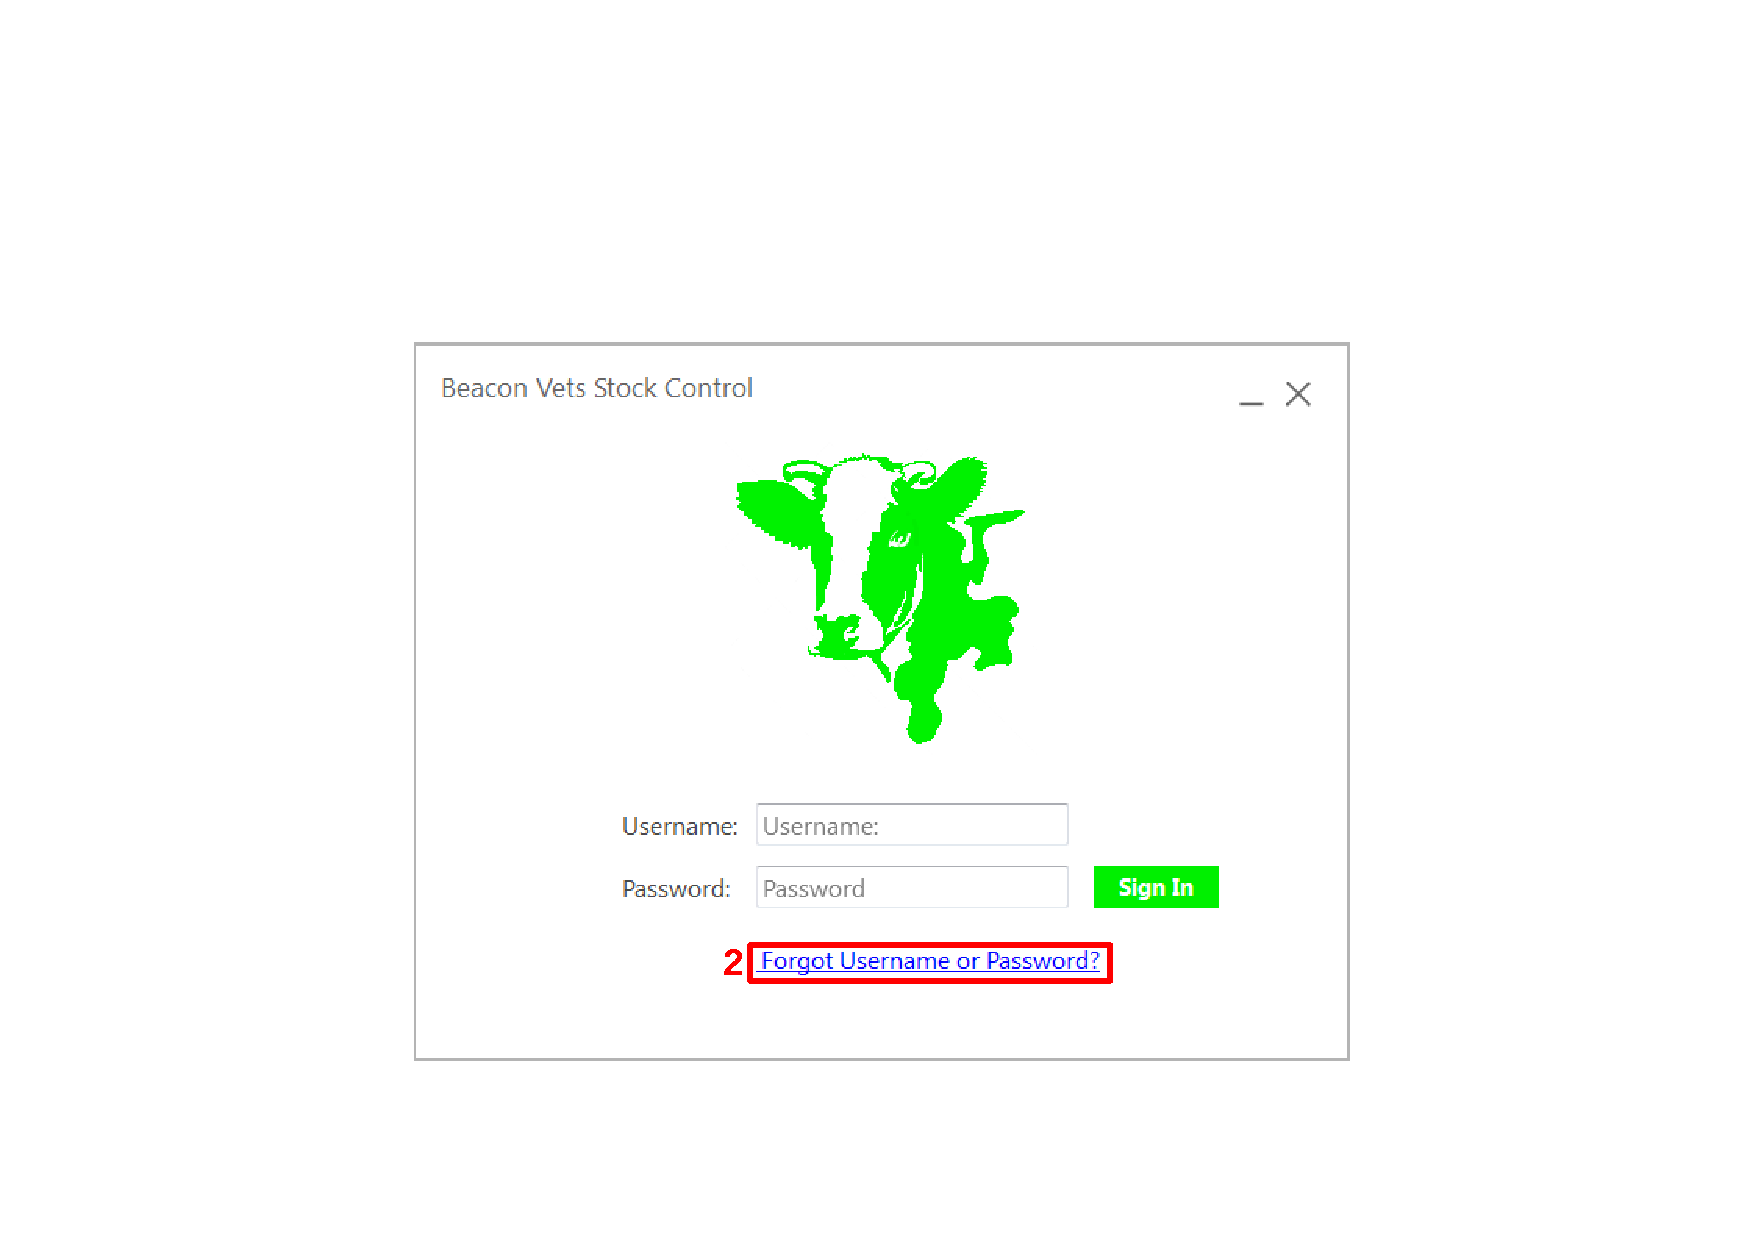
\includegraphics[width=8cm]{./ManualImages/forgot-password-1.pdf}

this will take you to the forgot password screen.

\textbf{3.} Enter the email address associated with your account.

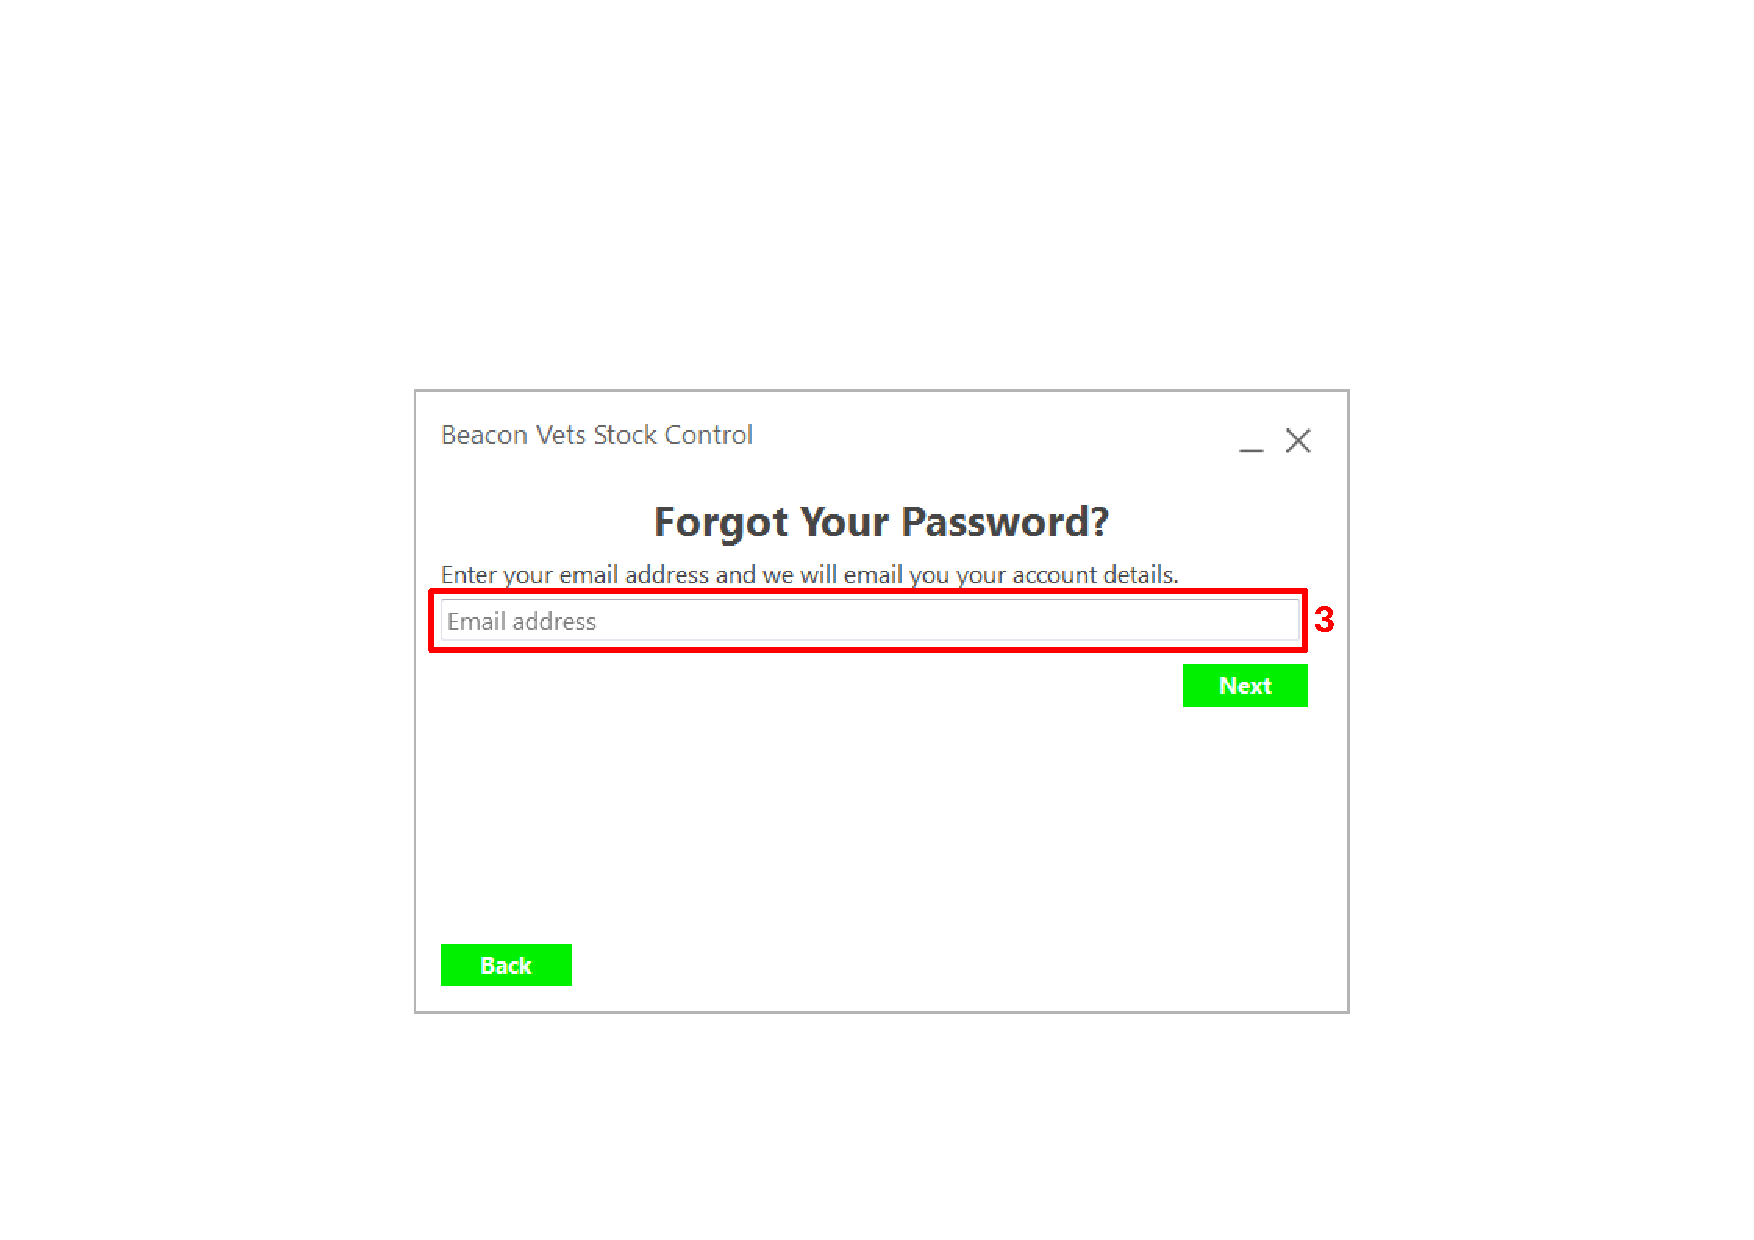
\includegraphics[width=8cm]{./ManualImages/forgot-password-2.pdf}

If you cannot remember the email address associated to your account, another employee can sign in and locate the email address associated to your account by using the search window.

For a tutorial on using the search window, go to page .

\textbf{4.} Click the `Next' button.

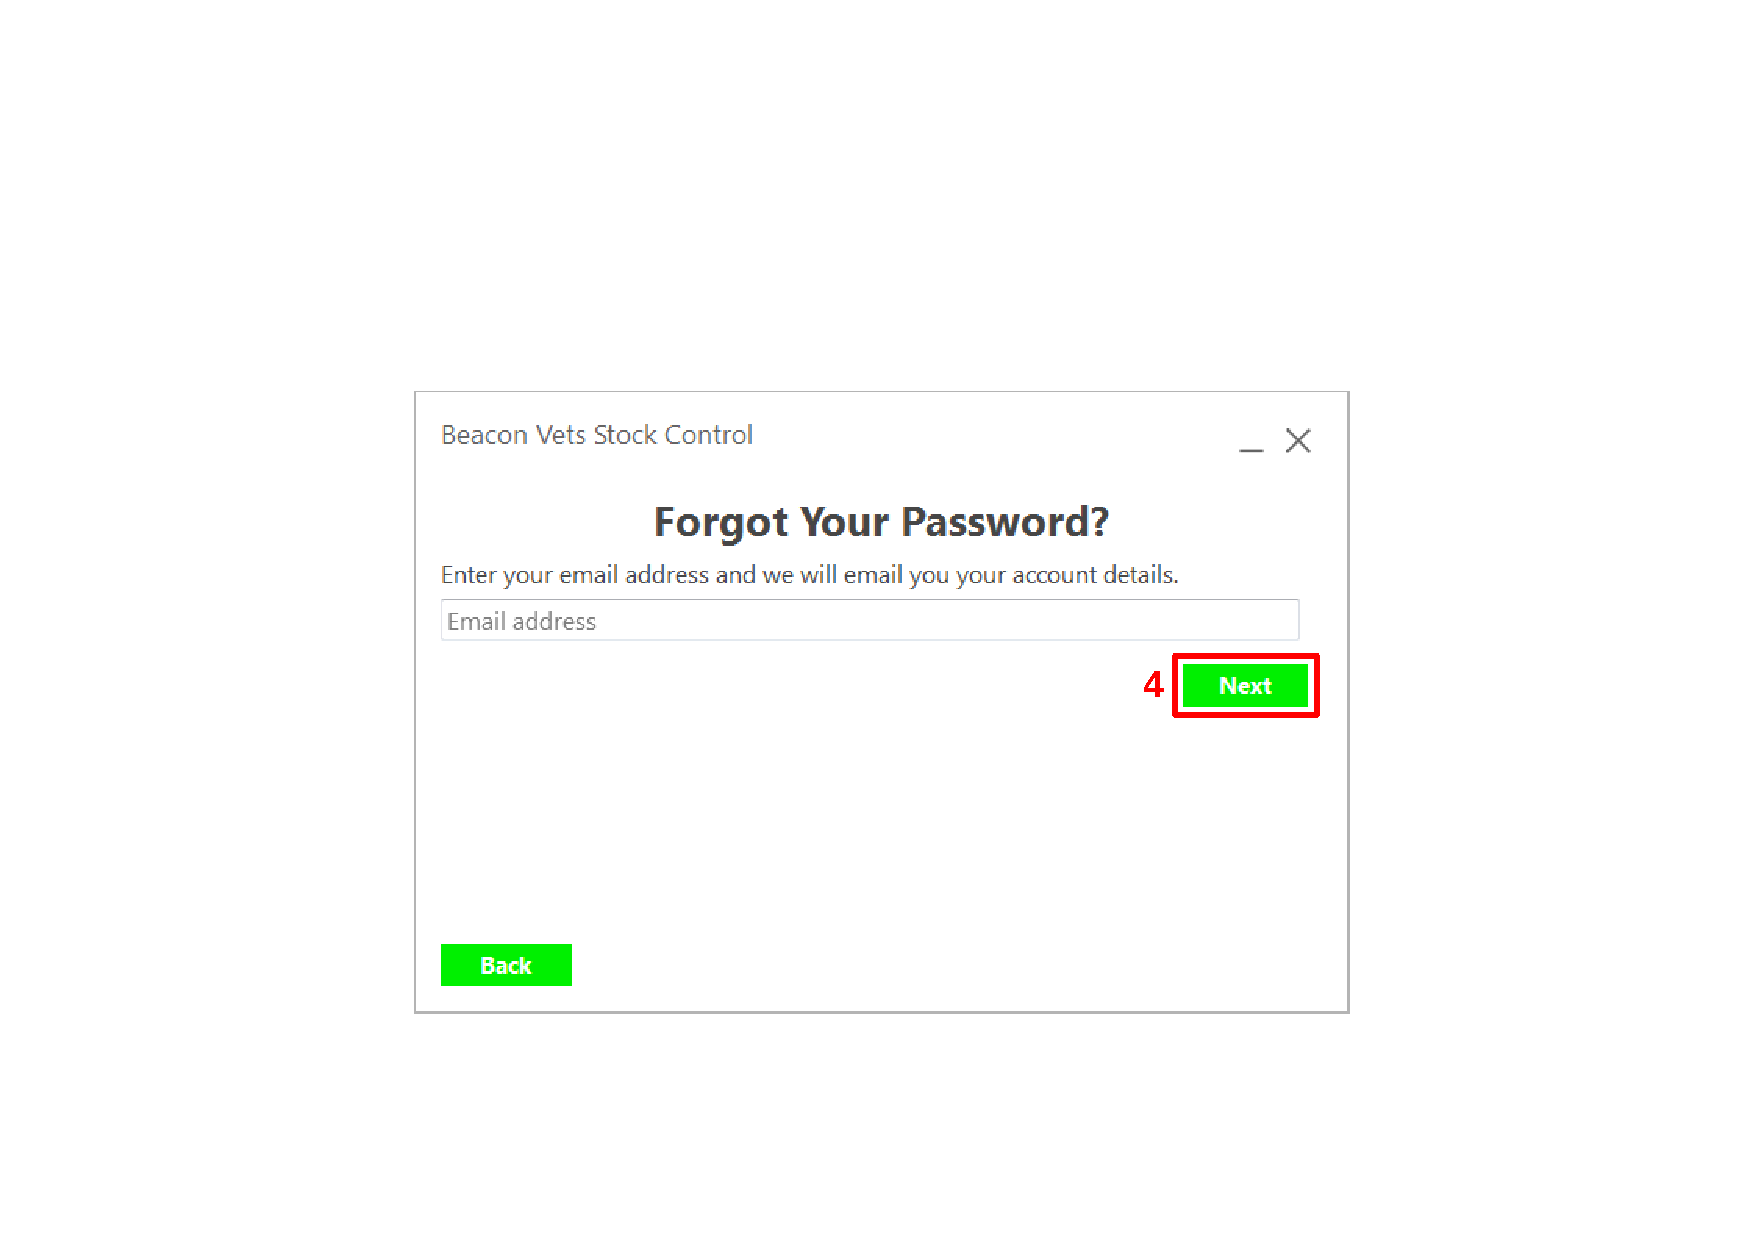
\includegraphics[width=8cm]{./ManualImages/forgot-password-3.pdf}

If the email address you entered is associated to your account, then the system will send an email to that email address, containing your user-name and password.

\textbf{5.} Check your email inbox. If you did not received the email, first check your spam or junk folder and if the email is not in there, repeat step 3 and 4.

If you can no longer access the email address associated to your account, go to page \pageref{fig:Unable to access your email address}.

\pagebreak
\subsubsection{Unable to access your email address}
\label{fig:Unable to access your email address}

If you are unable to access the email address associated to your account, the administrator must log into their account on the system. They must then change the email address associated to your account, to one in which you do have access to. For a tutorial on how to do this, go to page .

\pagebreak
\subsubsection{Adding a Product to the system}
\label{fig:Adding a Product to the system}

\textbf{1.} Log into the system.

If you do not know how to log into the system, the tutorial on how to log into the system can be found on page \pageref{fig:Logging into the system}.

\textbf{2.} On any interface, click on the product option in the menu bar.

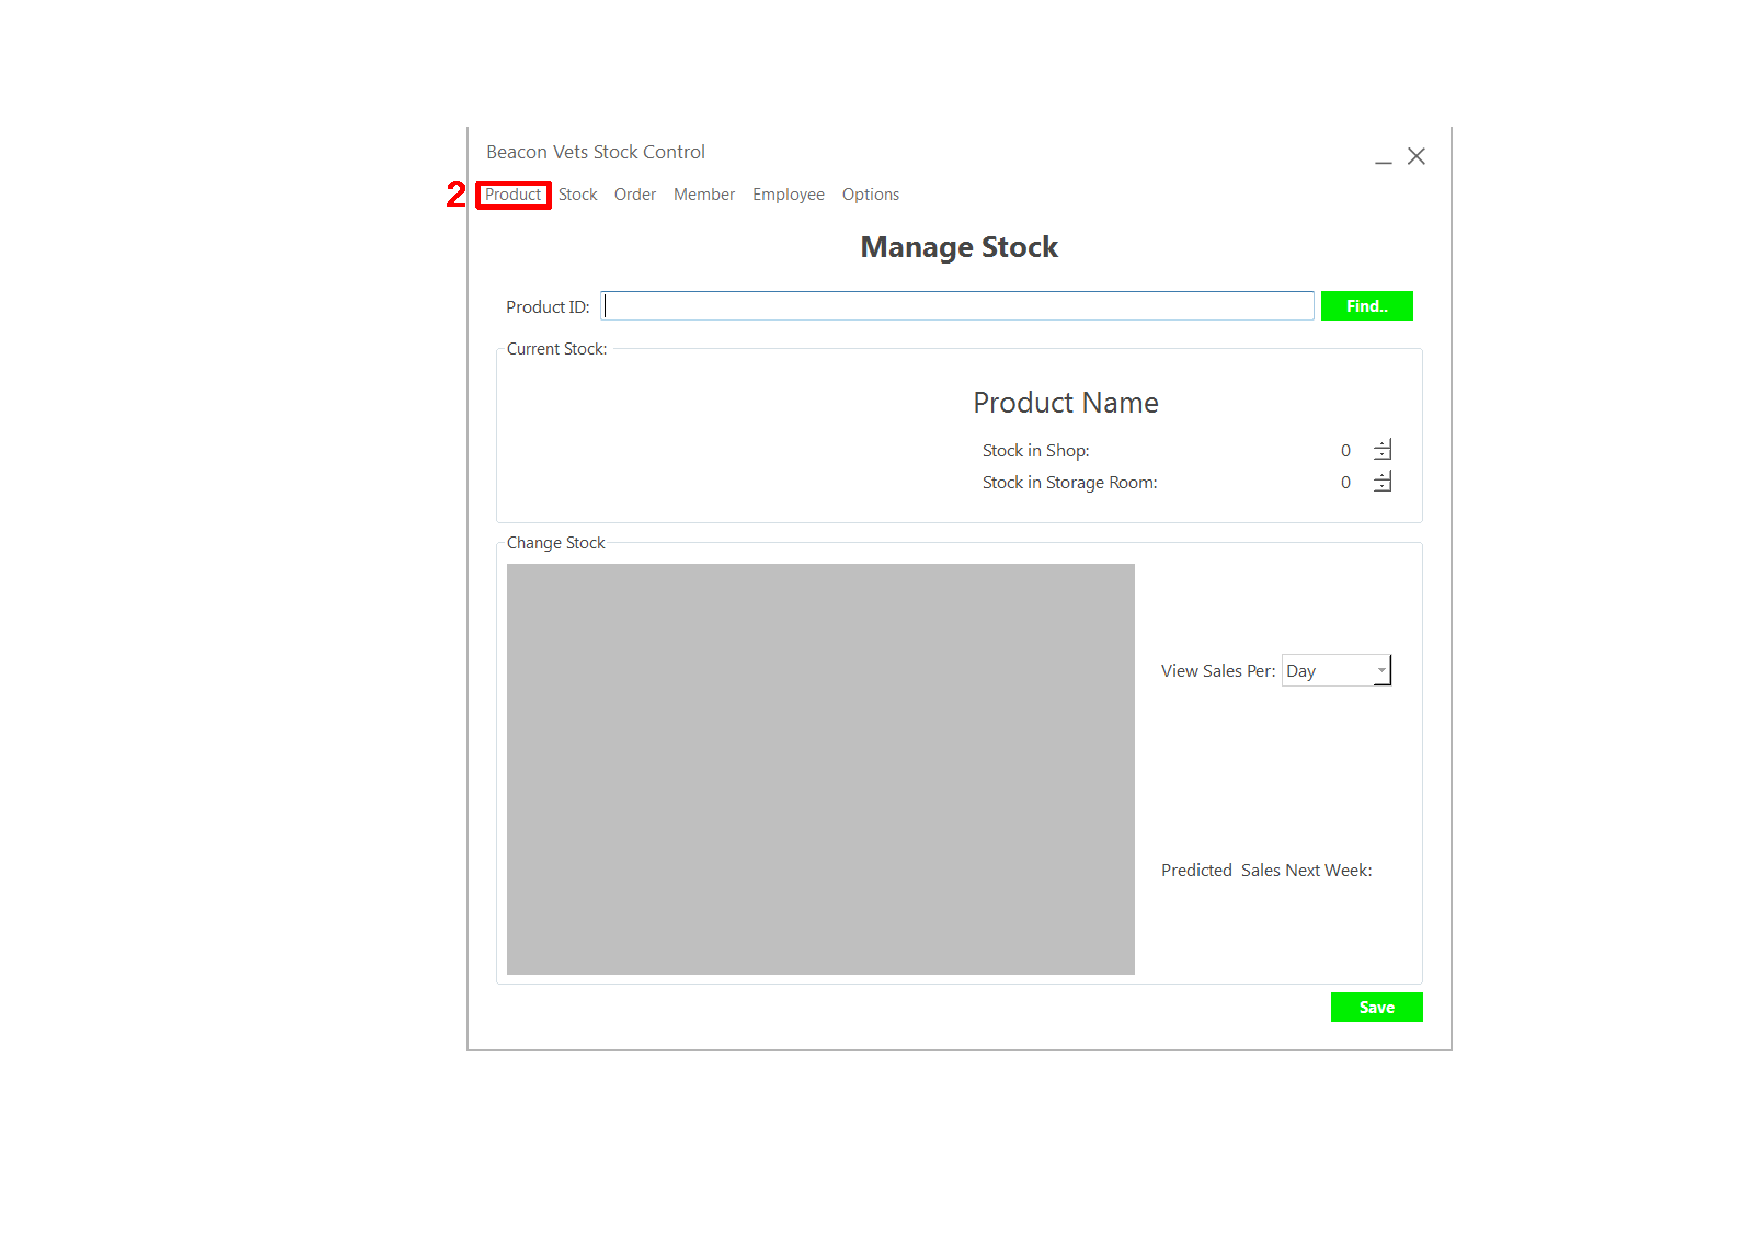
\includegraphics[width=8cm]{./ManualImages/add-product-1.pdf}

\textbf{3.} Click on the `Add a New Product' option from the drop down menu.

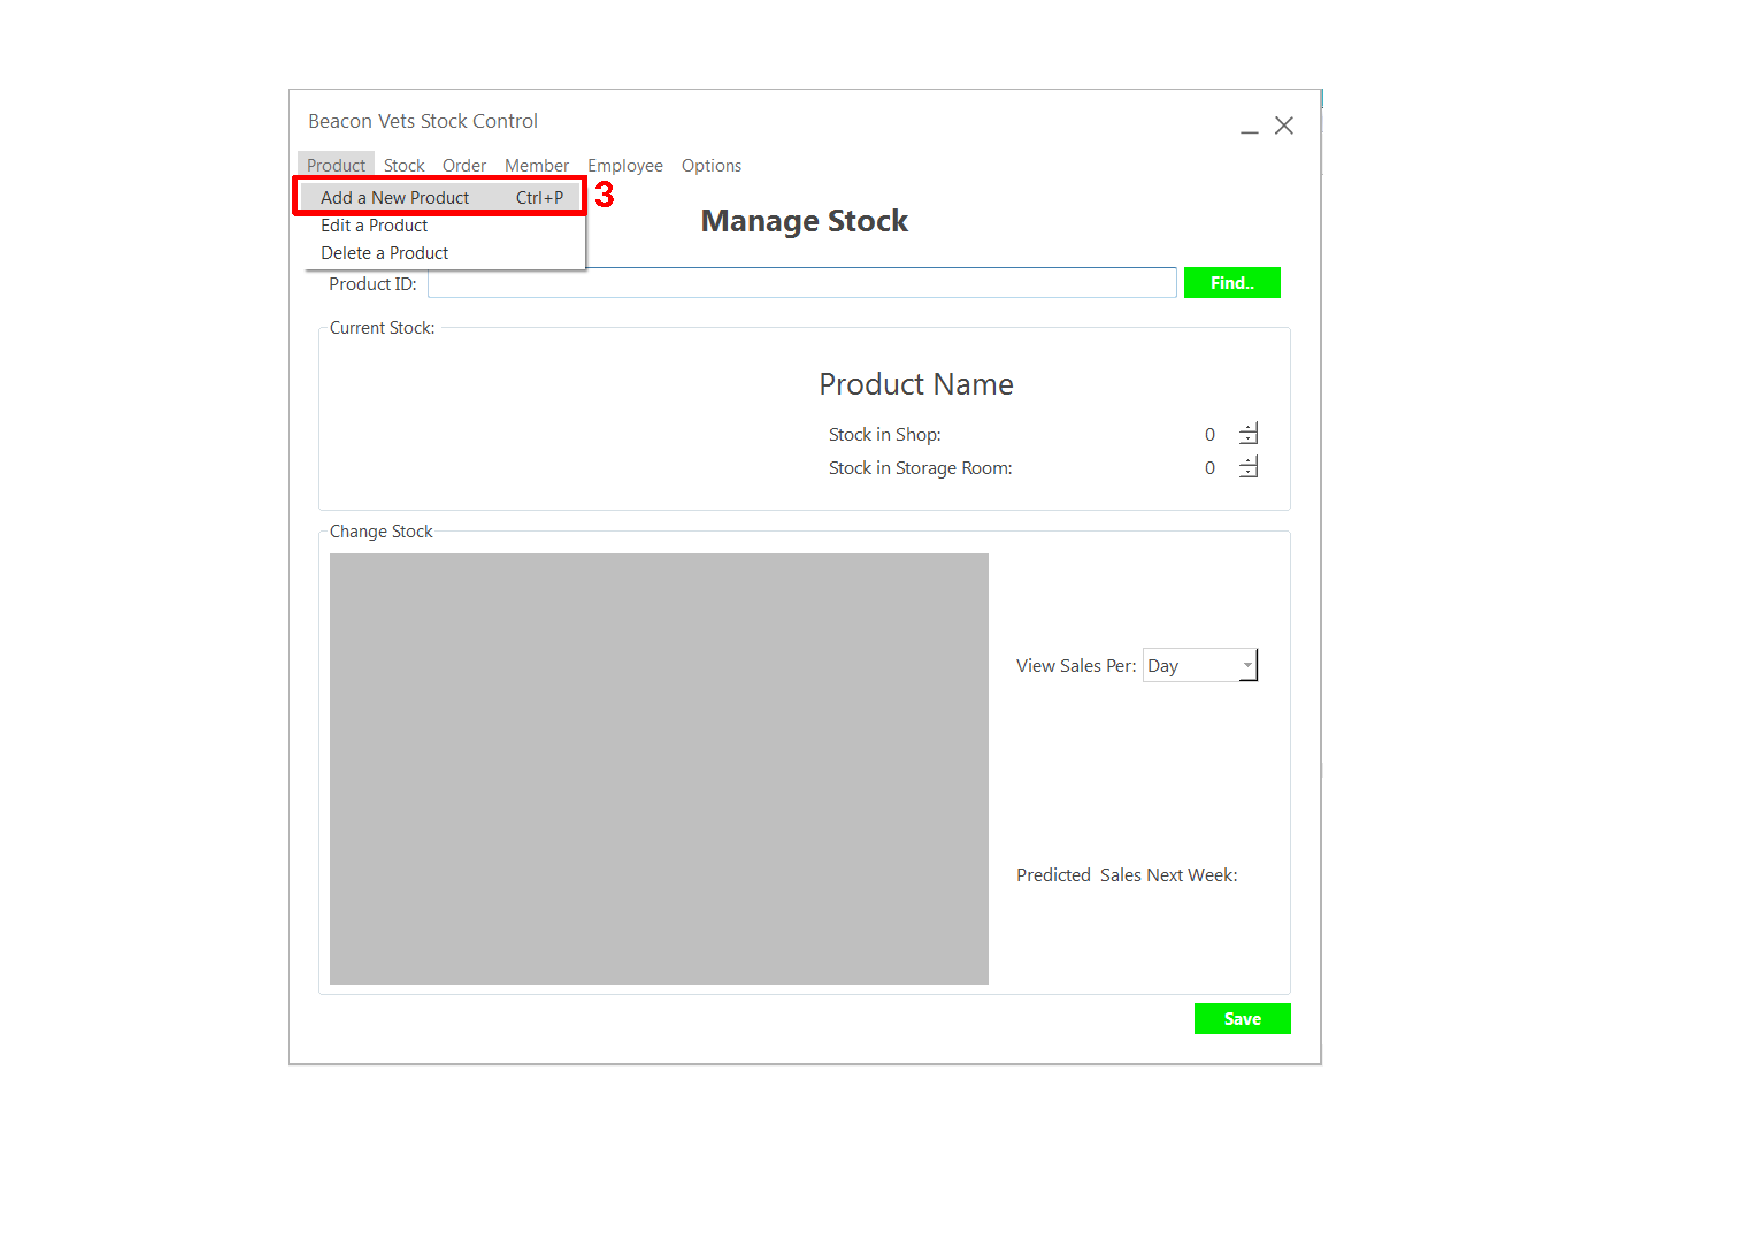
\includegraphics[width=8cm]{./ManualImages/add-product-2.pdf}

An alternative to step 2 and step 3, is by pressing the `CTRL' and `P' button on the keyboard simultaneously.

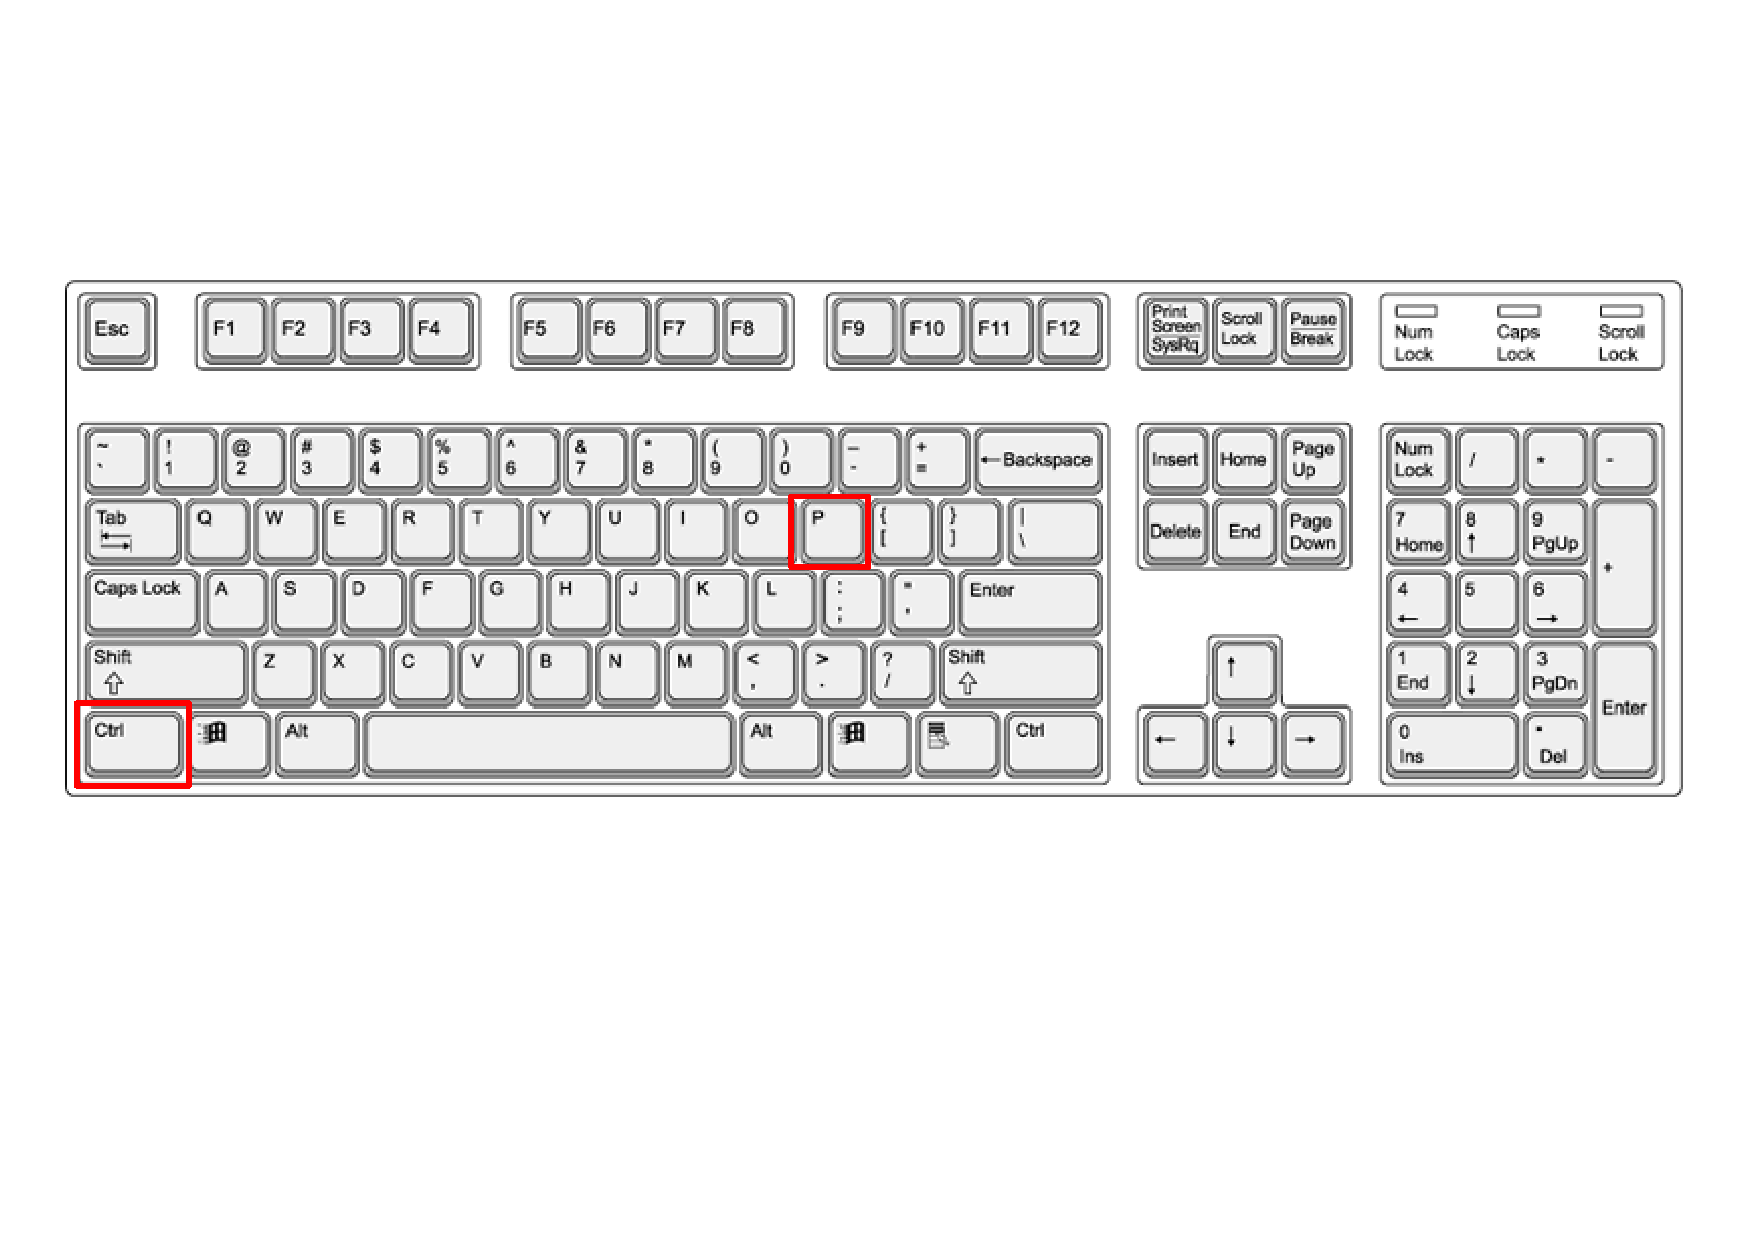
\includegraphics[width=\textwidth]{./ManualImages/shortcut-product.pdf}

\textbf{4. }Enter data into the data fields.

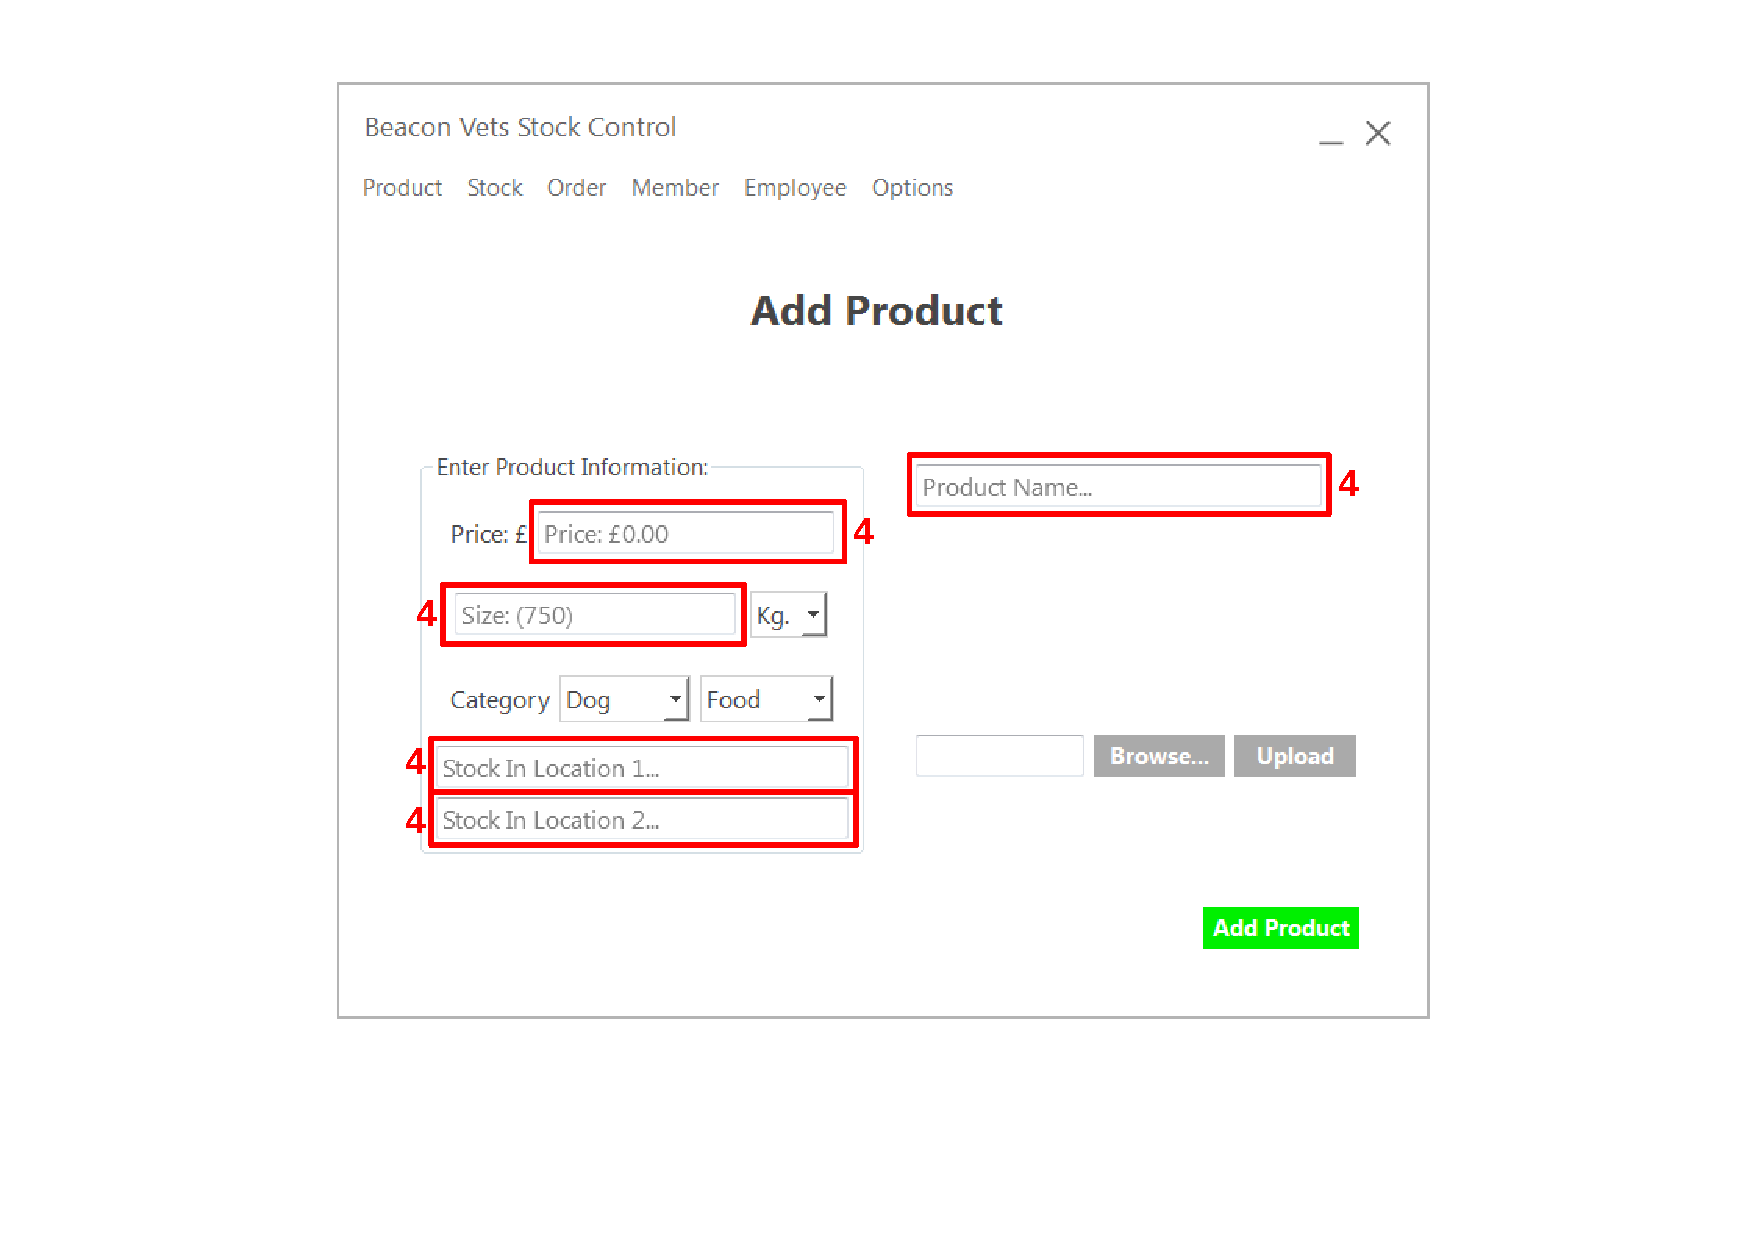
\includegraphics[width=8cm]{./ManualImages/add-product-3.pdf}

\textbf{5.} Choose the appropriate option in the drop down menus.

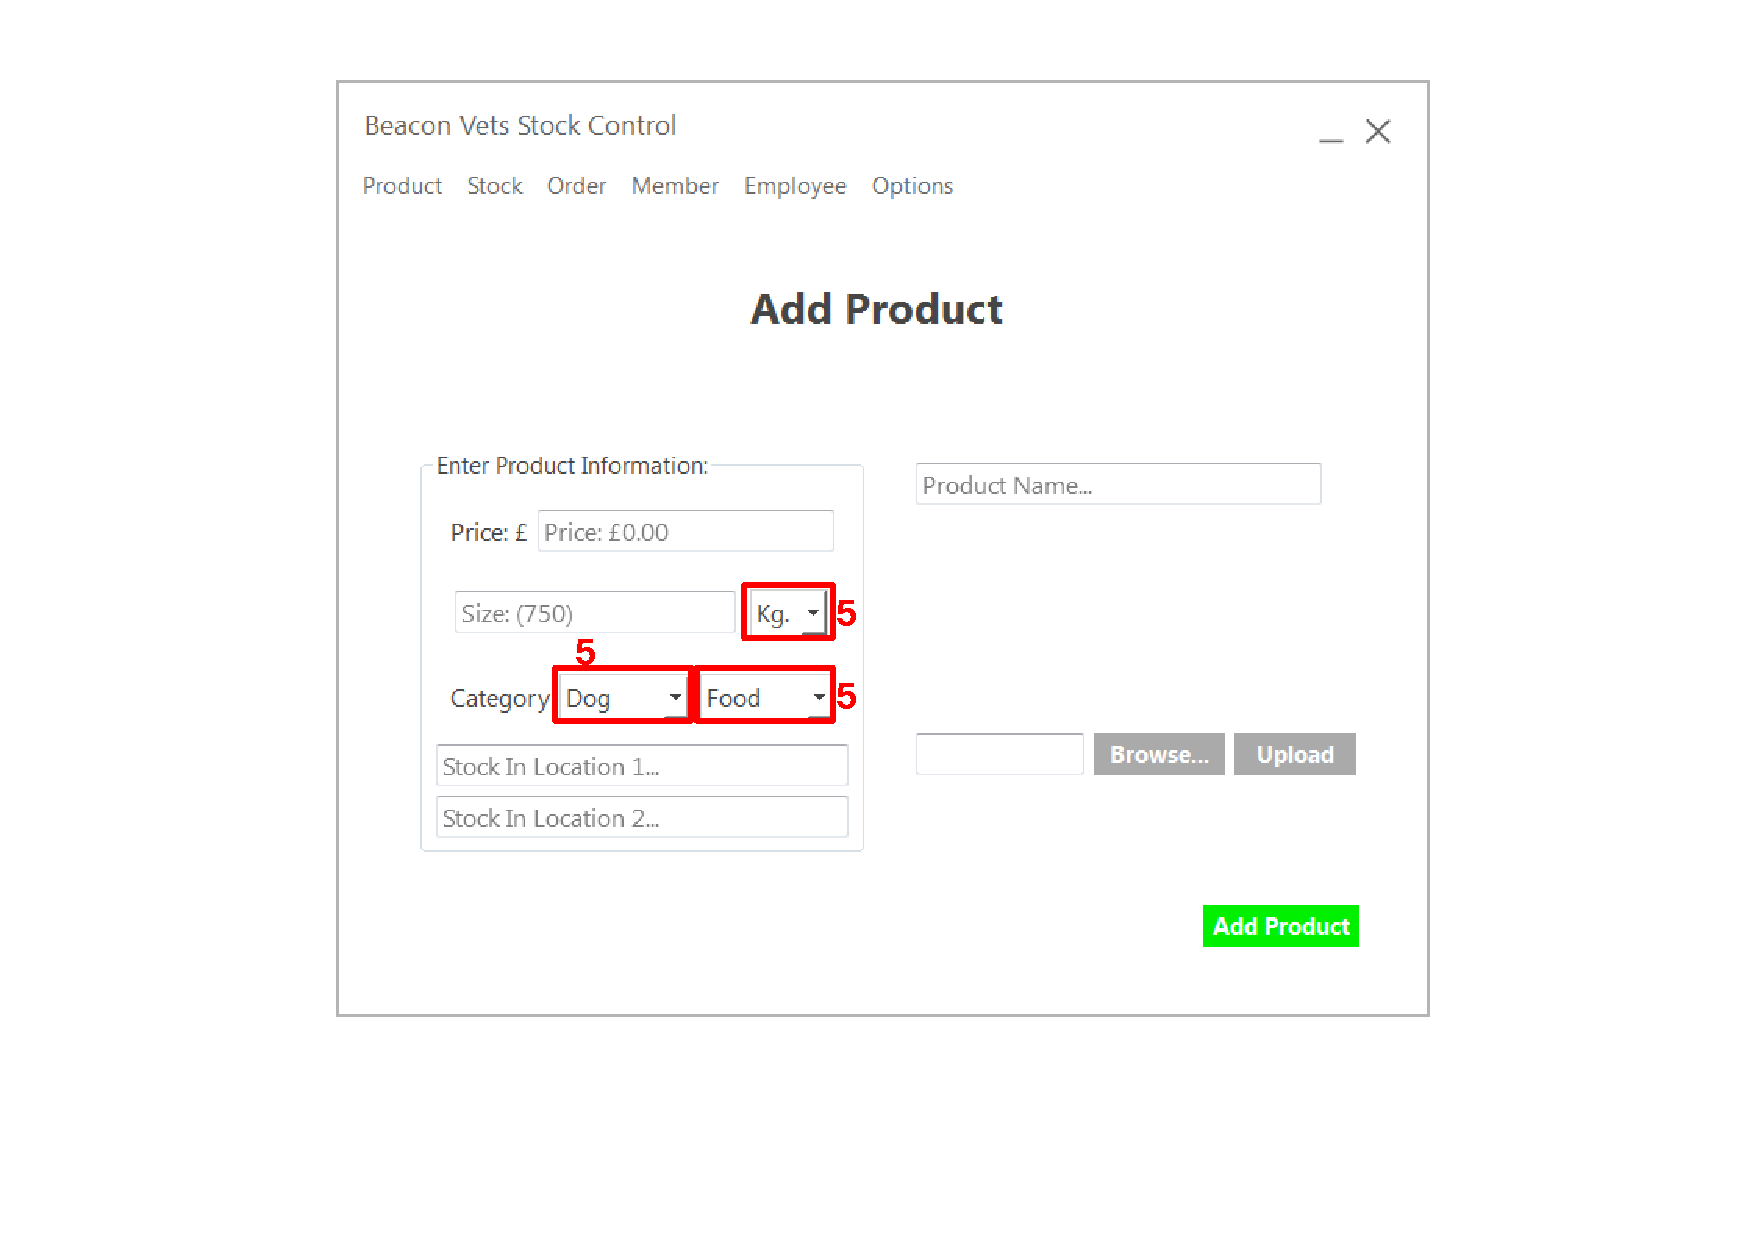
\includegraphics[width=8cm]{./ManualImages/add-product-4.pdf}

\textbf{6.} Click on the browse button.

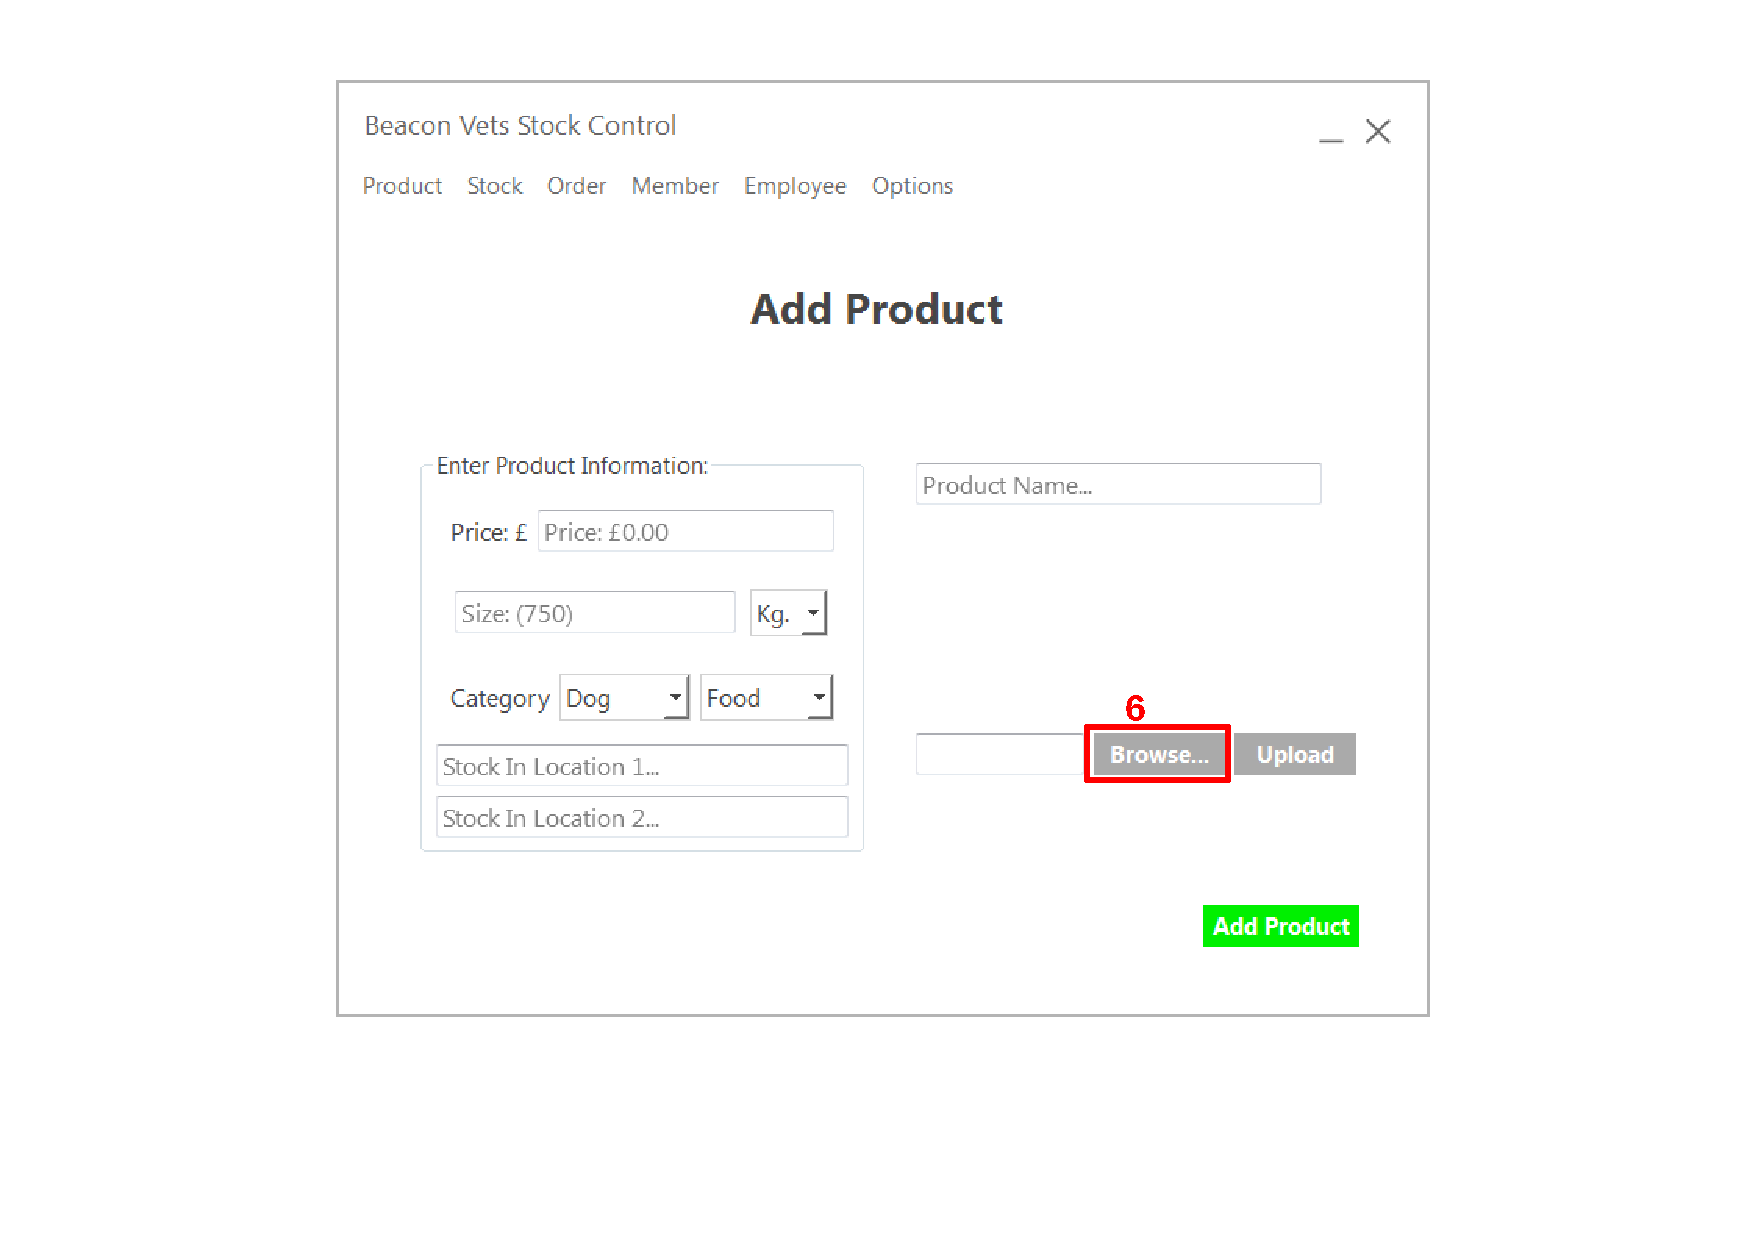
\includegraphics[width=8cm]{./ManualImages/add-product-5.pdf}

\textbf{7.} Choose an image to represent the product.

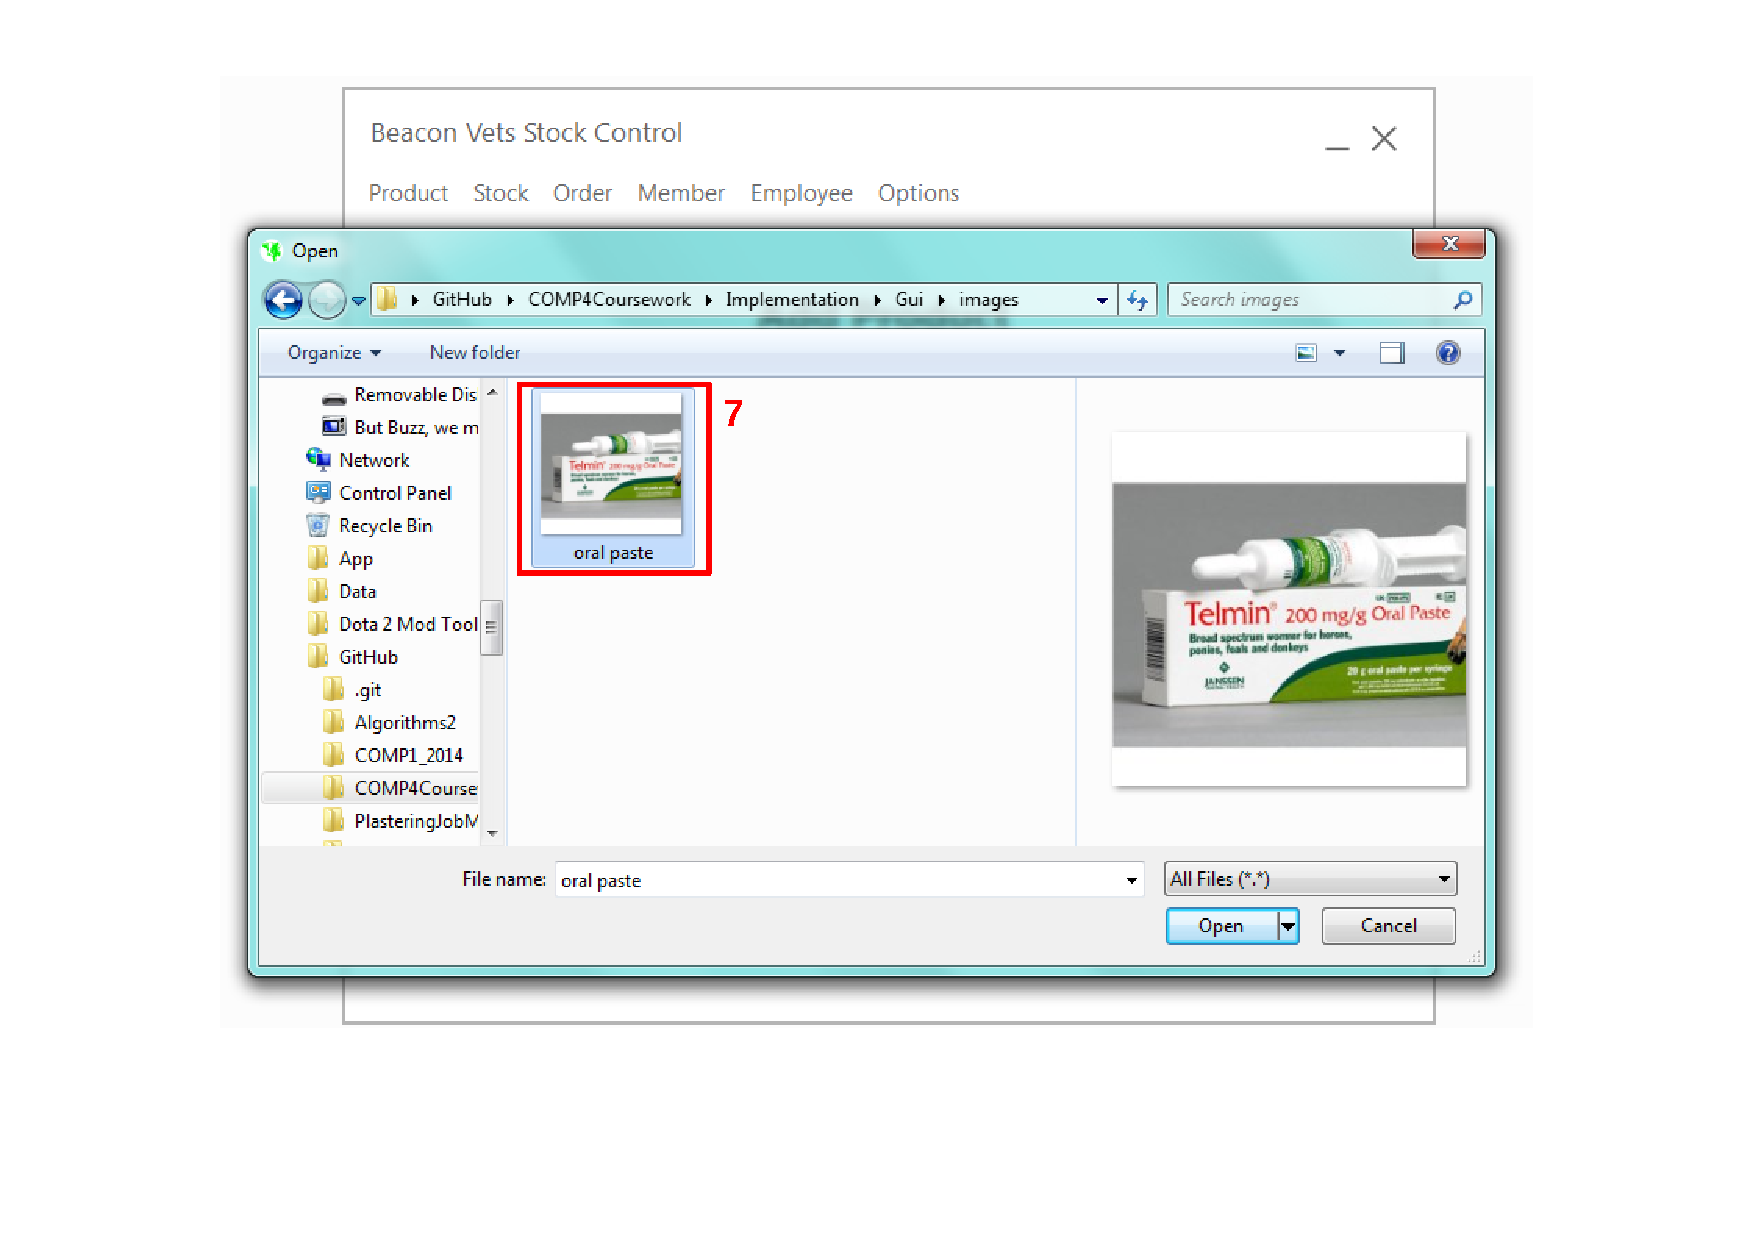
\includegraphics[width=8cm]{./ManualImages/add-product-6.pdf}

\textbf{8.} Click on the `Open' button.

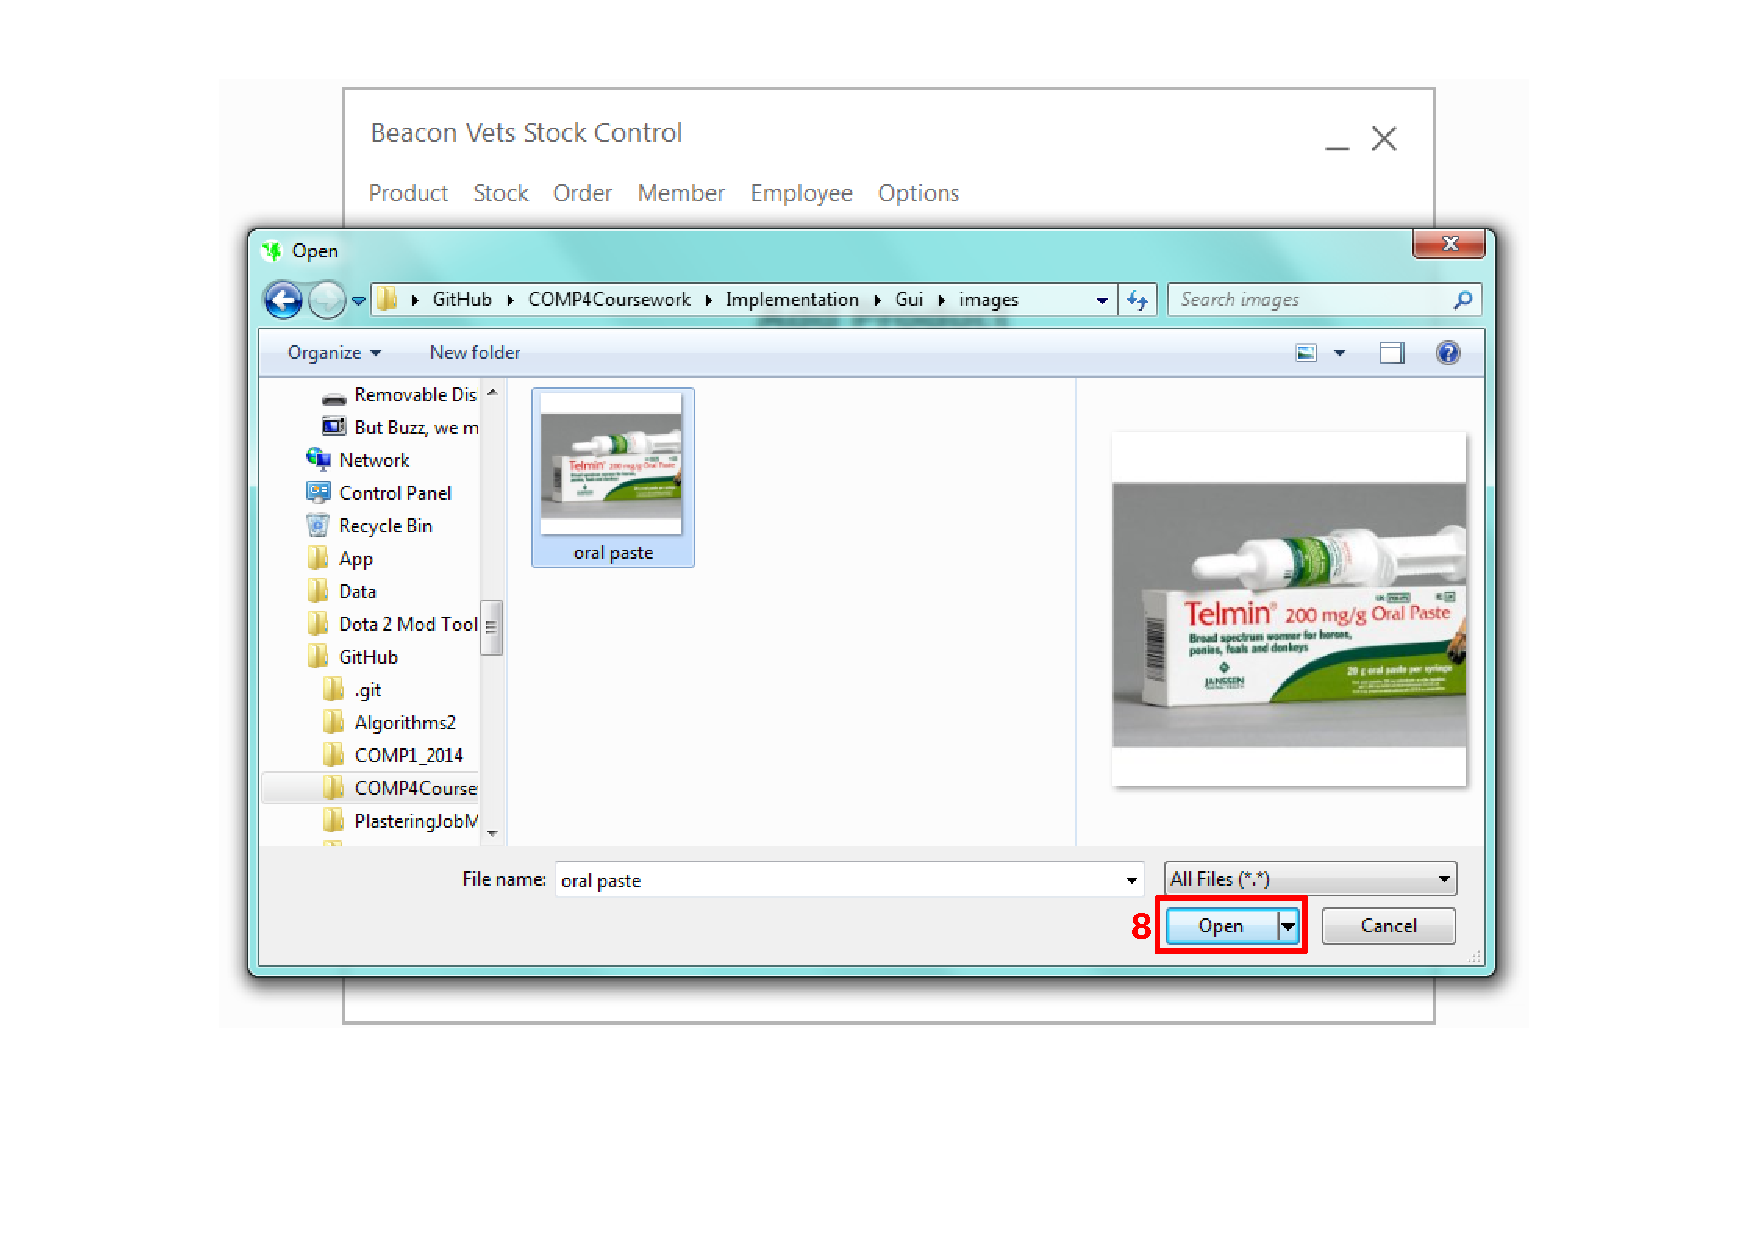
\includegraphics[width=8cm]{./ManualImages/add-product-7.pdf}

\textbf{9.} Click the `Upload' button.

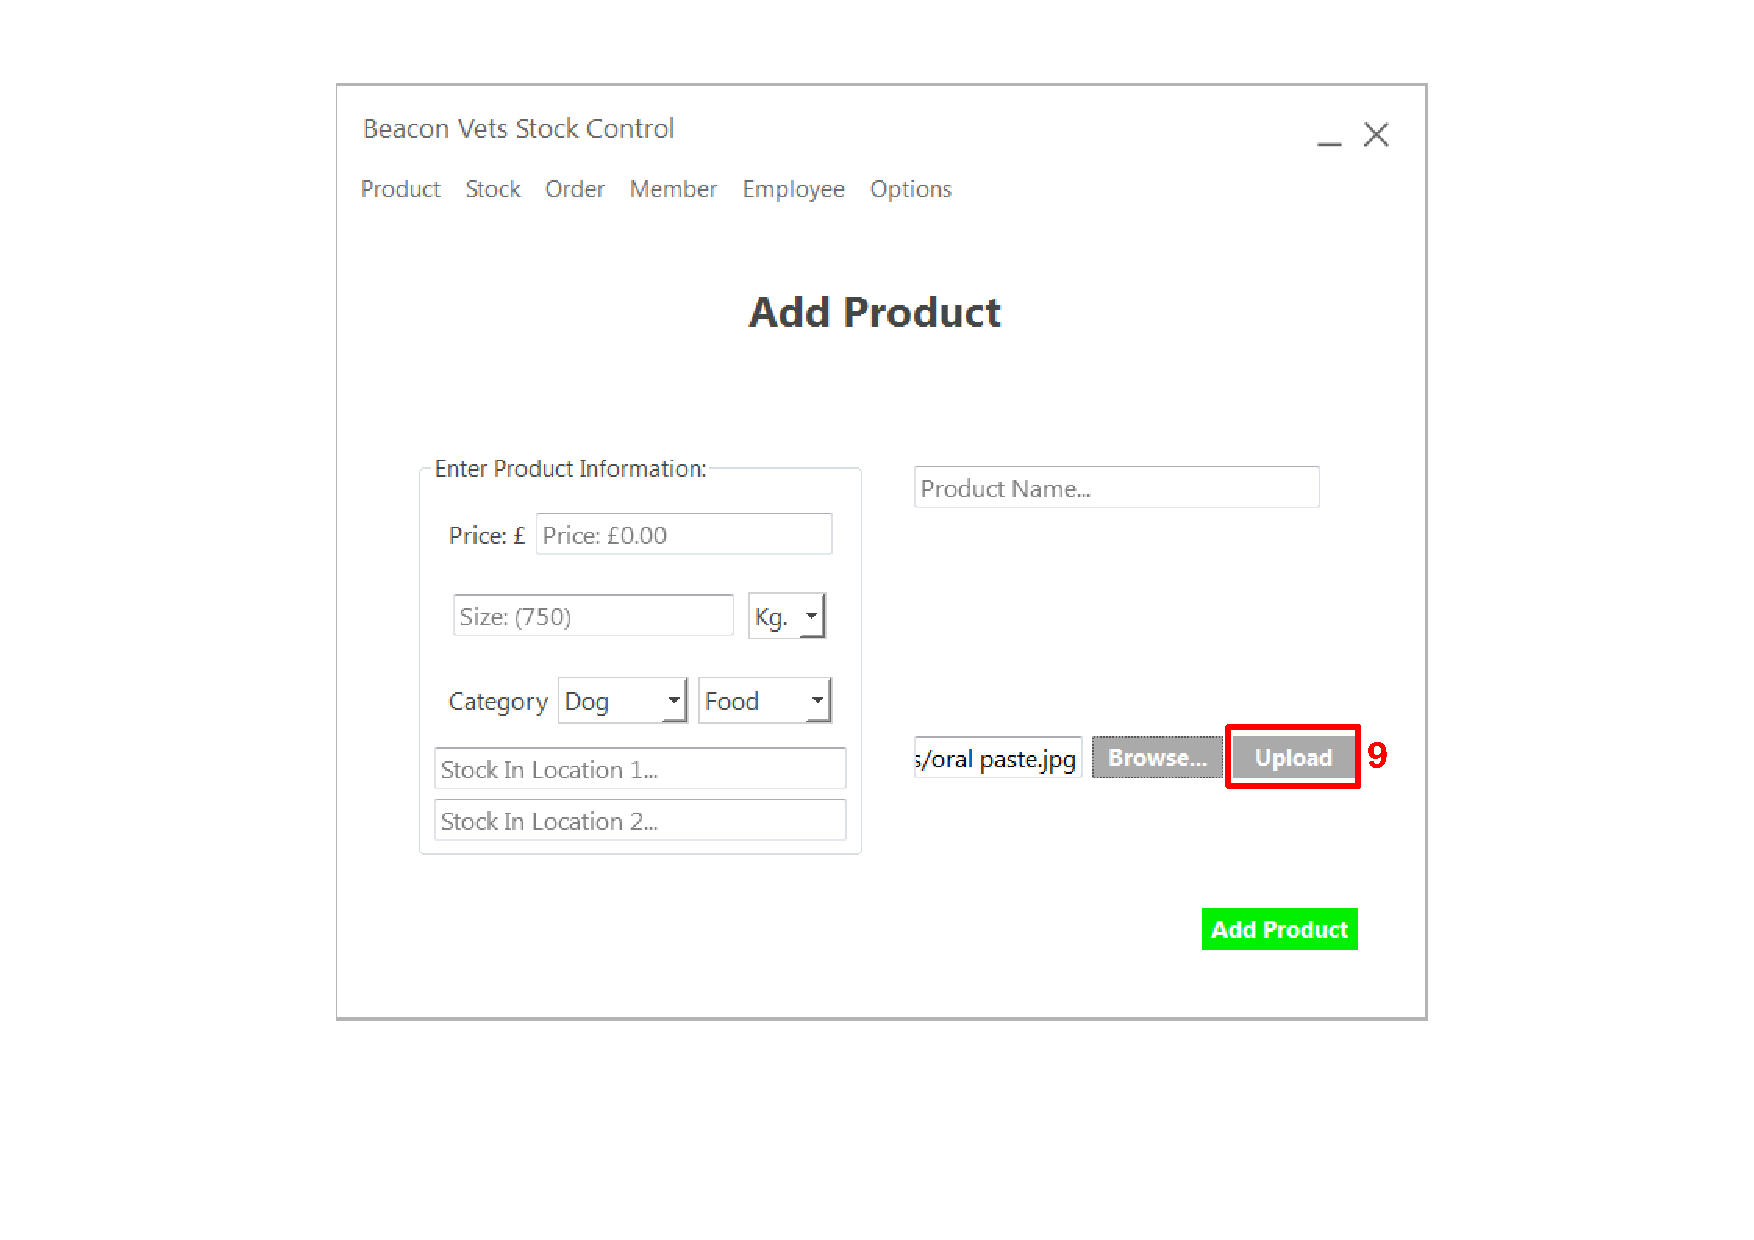
\includegraphics[width=8cm]{./ManualImages/add-product-8.pdf}

\textbf{10.} Click the `Add Product' button.

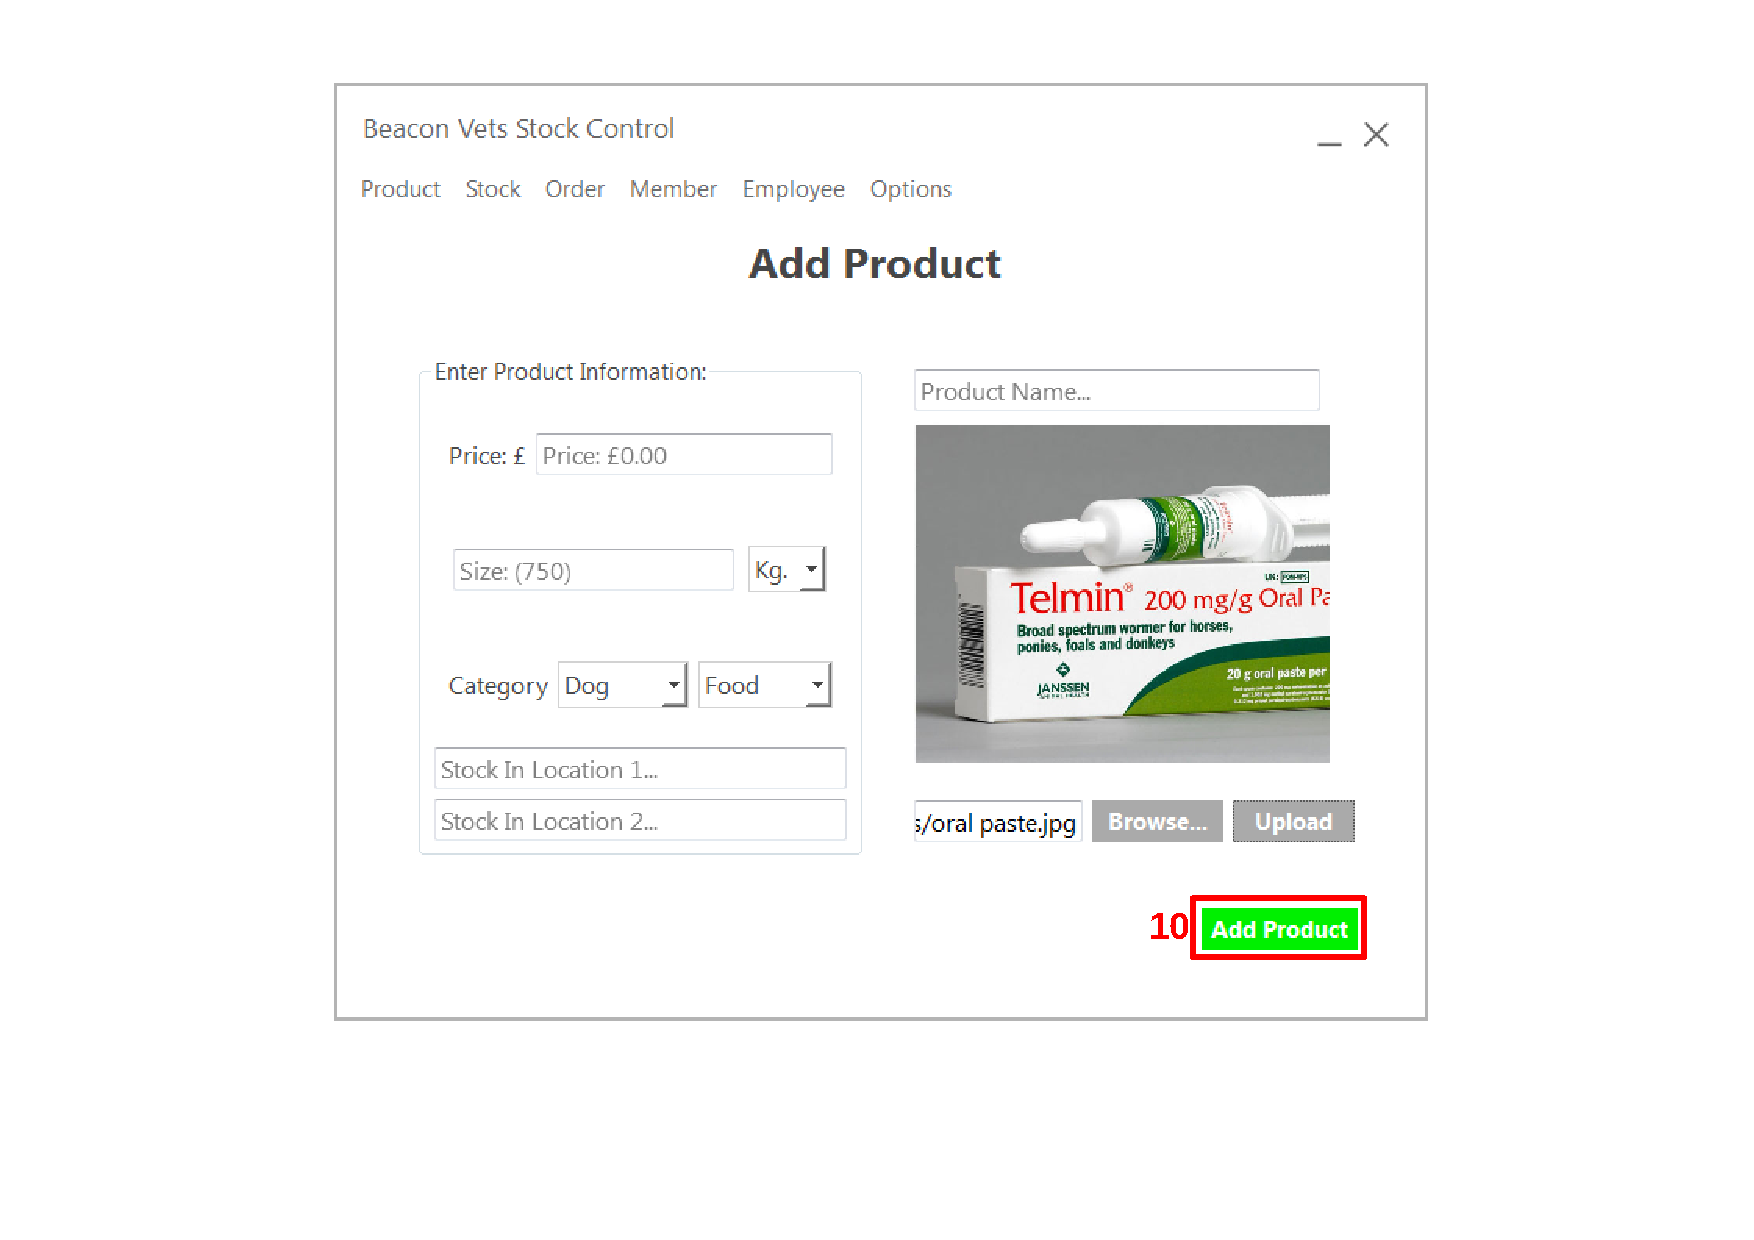
\includegraphics[width=8cm]{./ManualImages/add-product-9.pdf}

\textbf{11.} Click the `Yes' button in the pop up window.

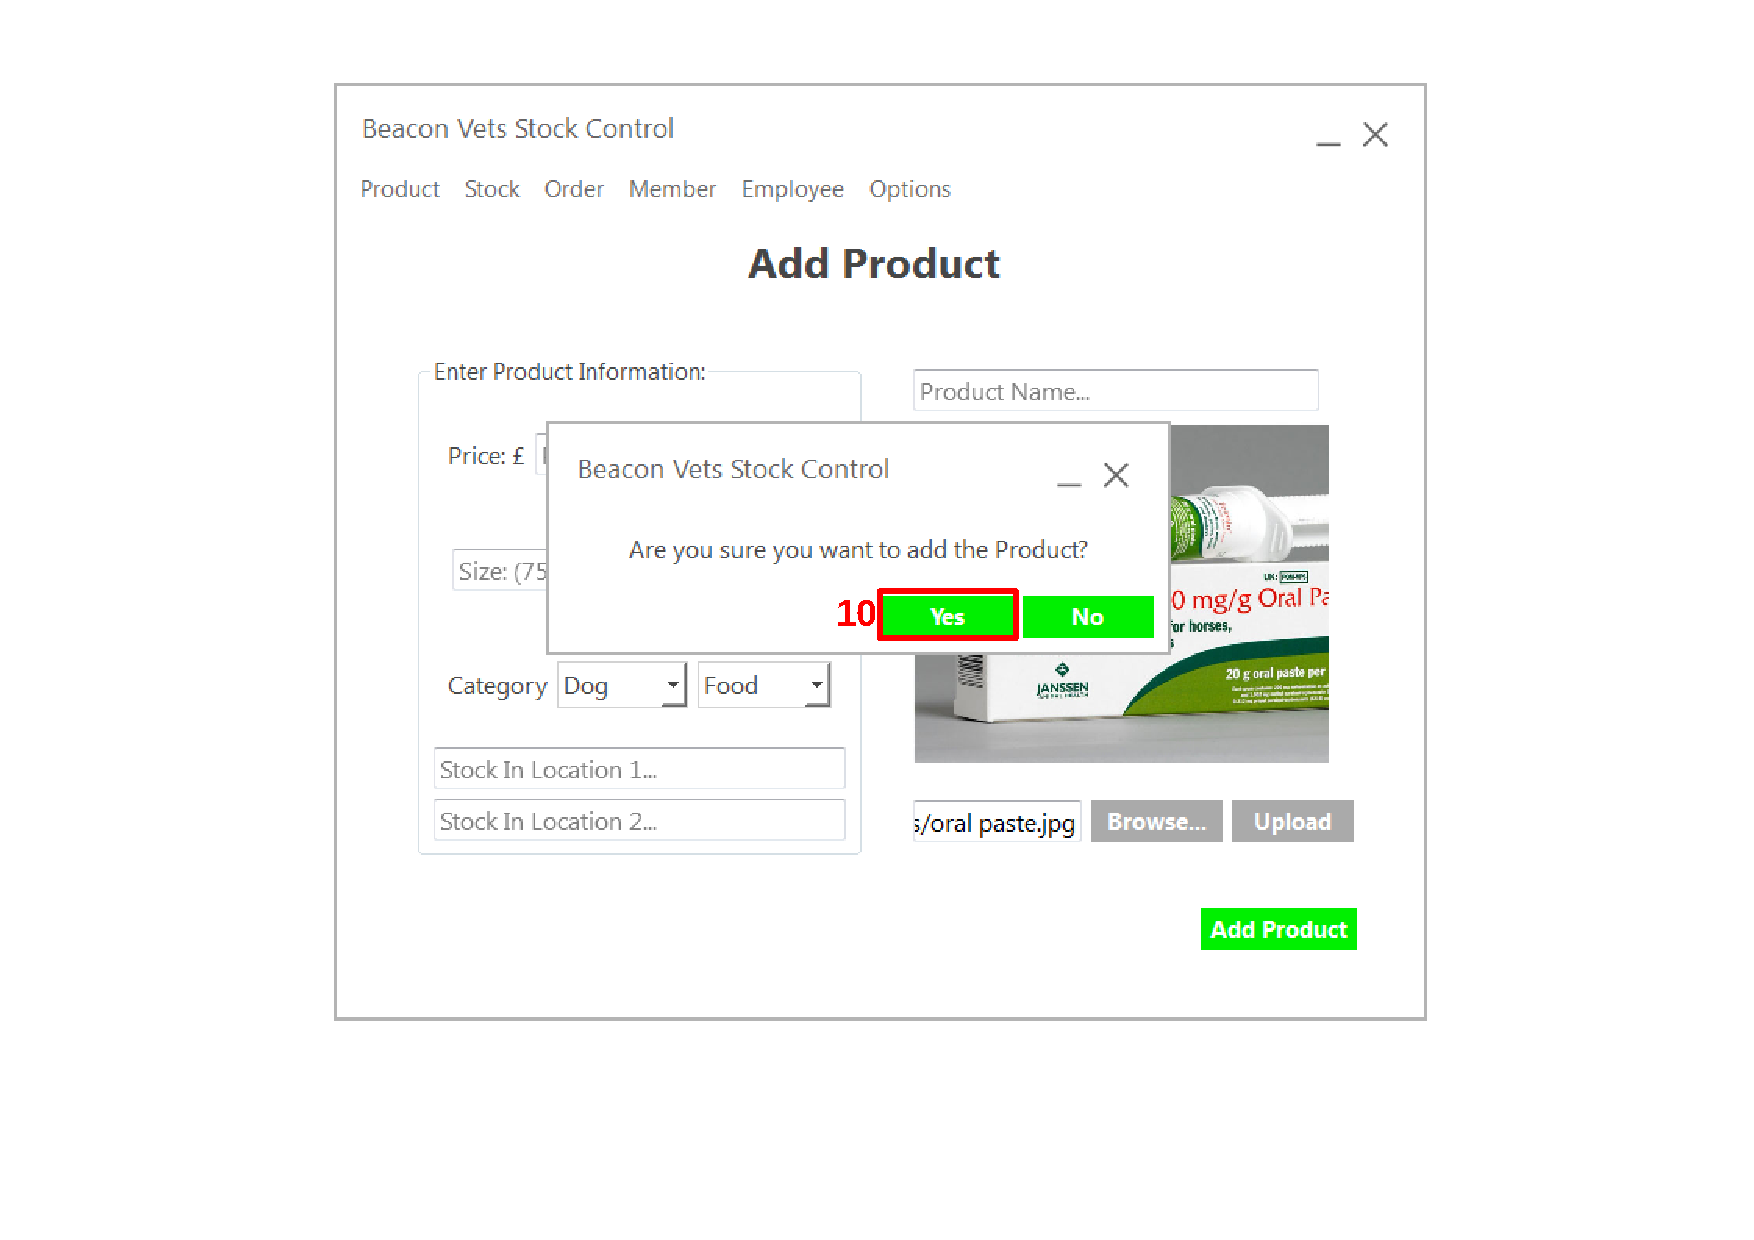
\includegraphics[width=8cm]{./ManualImages/add-product-10.pdf}

\textbf{12.} Click the `Ok' button in the pop up window.

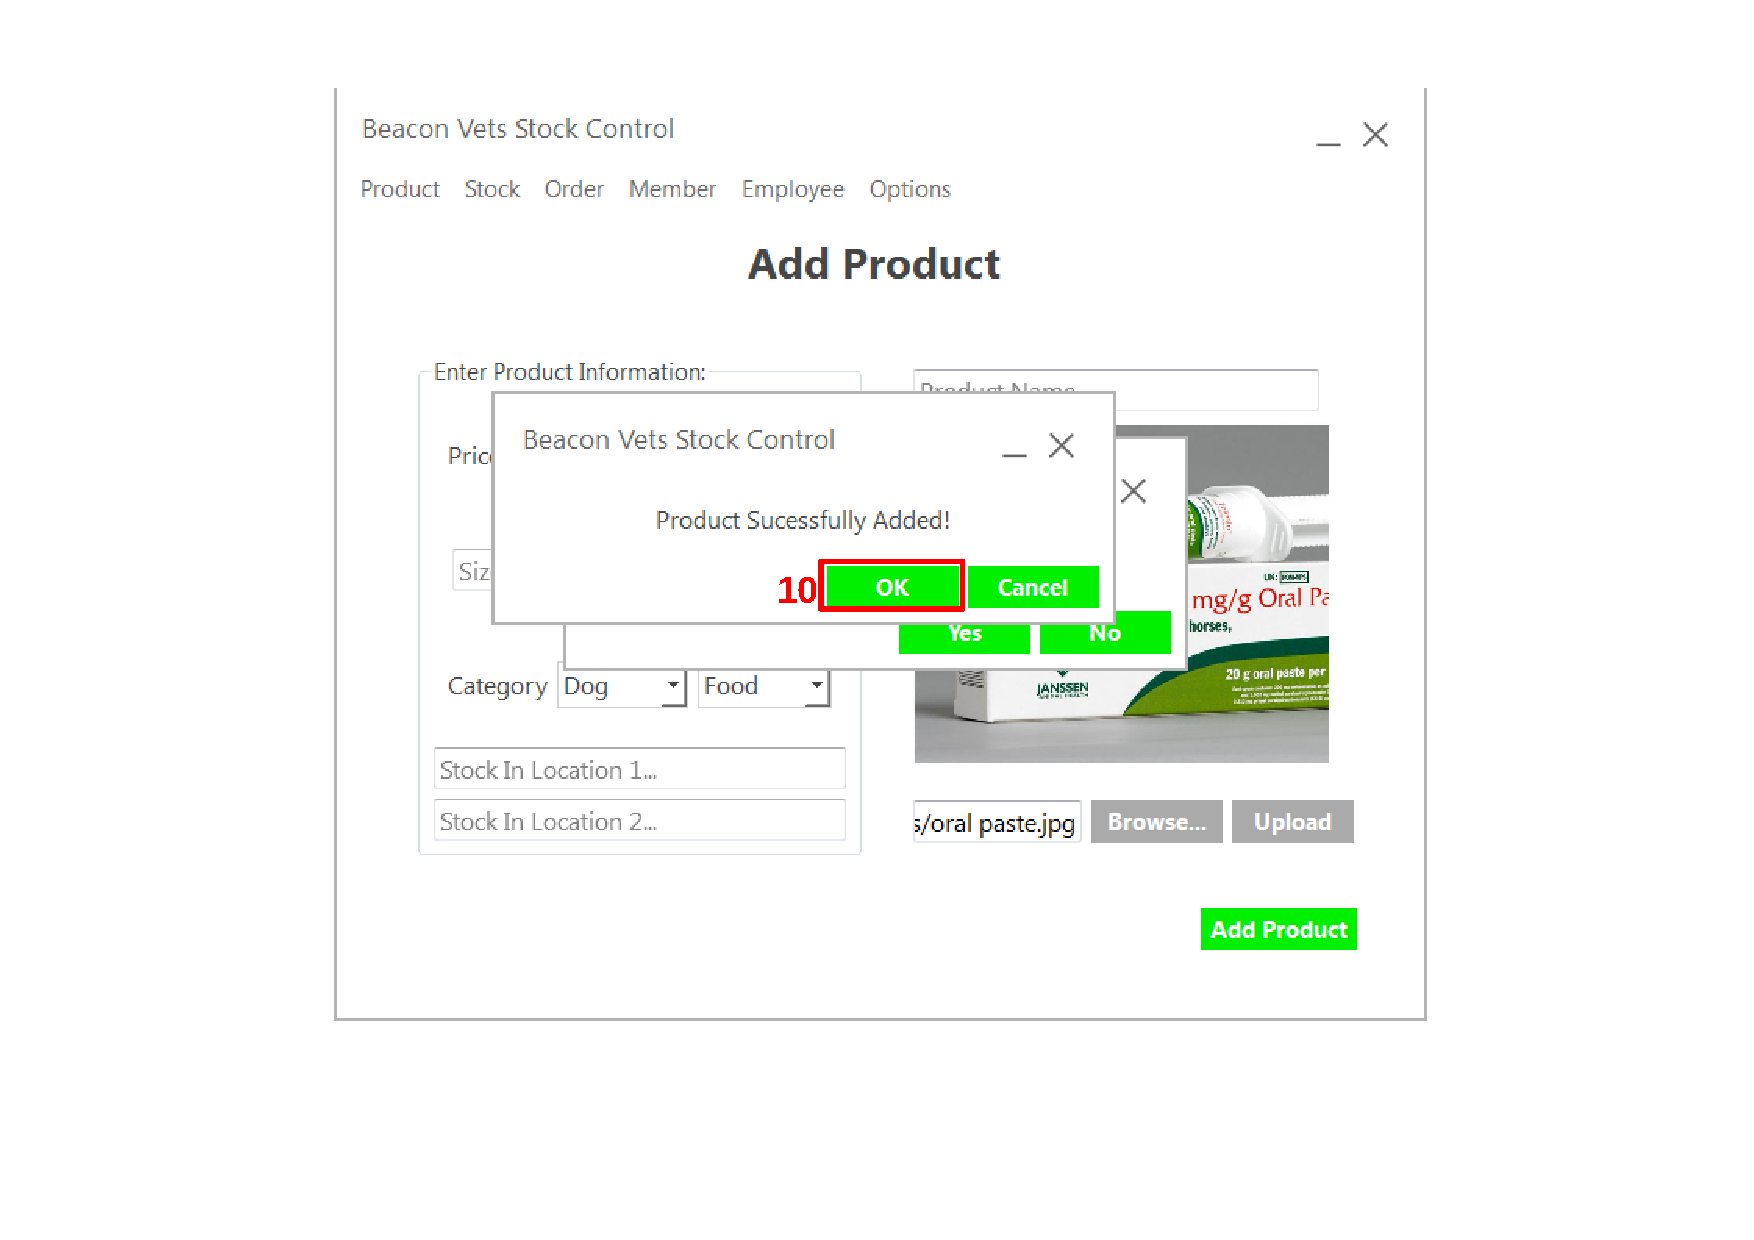
\includegraphics[width=8cm]{./ManualImages/add-product-11.pdf}

You have now successfully added a product to the database.

\pagebreak
\subsubsection{Adding a Member to the system}
\label{fig:Adding a Member to the system}

\textbf{1.} On any interface, click on the `Member' option in the menu-bar.

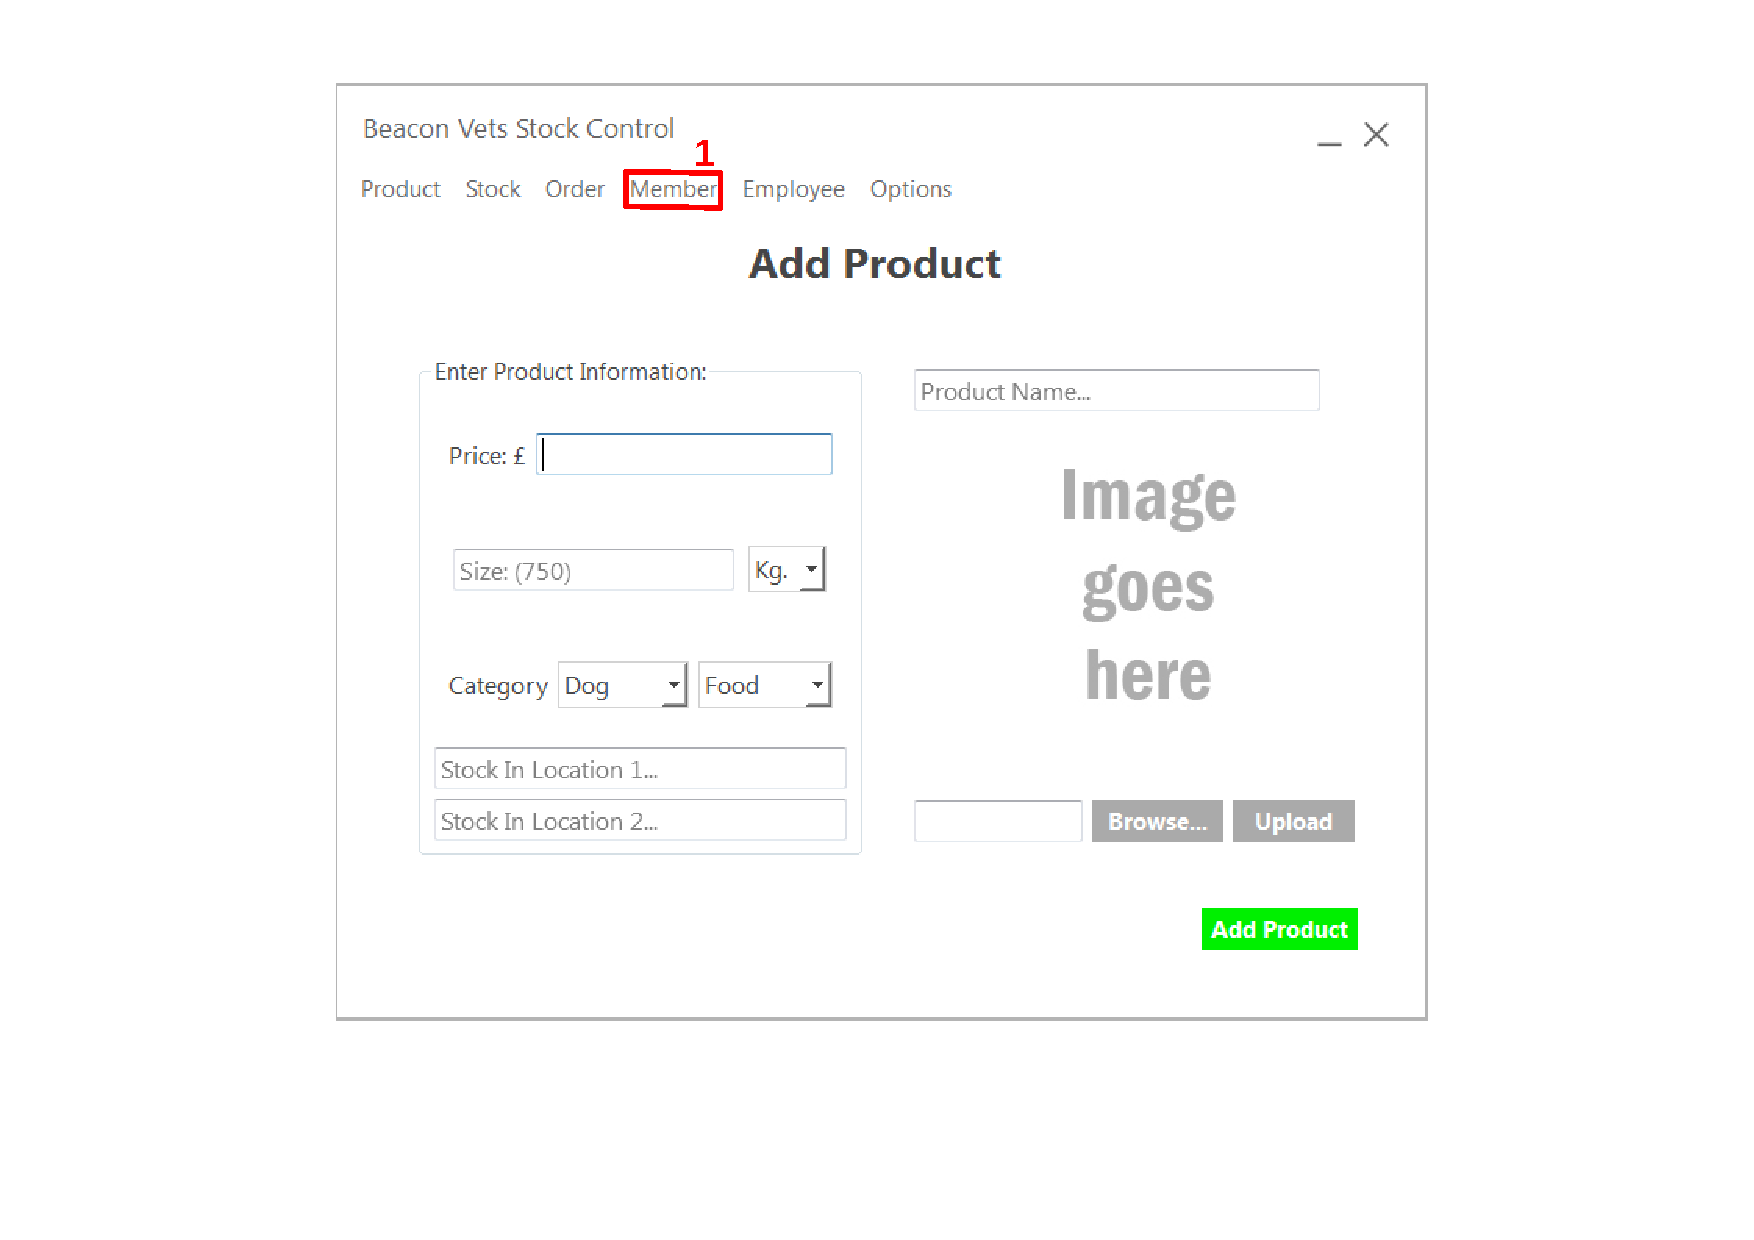
\includegraphics[width=8cm]{./ManualImages/add-member-1.pdf}

\textbf{2.} On the drop down menu, click on the `Add New Member' option.

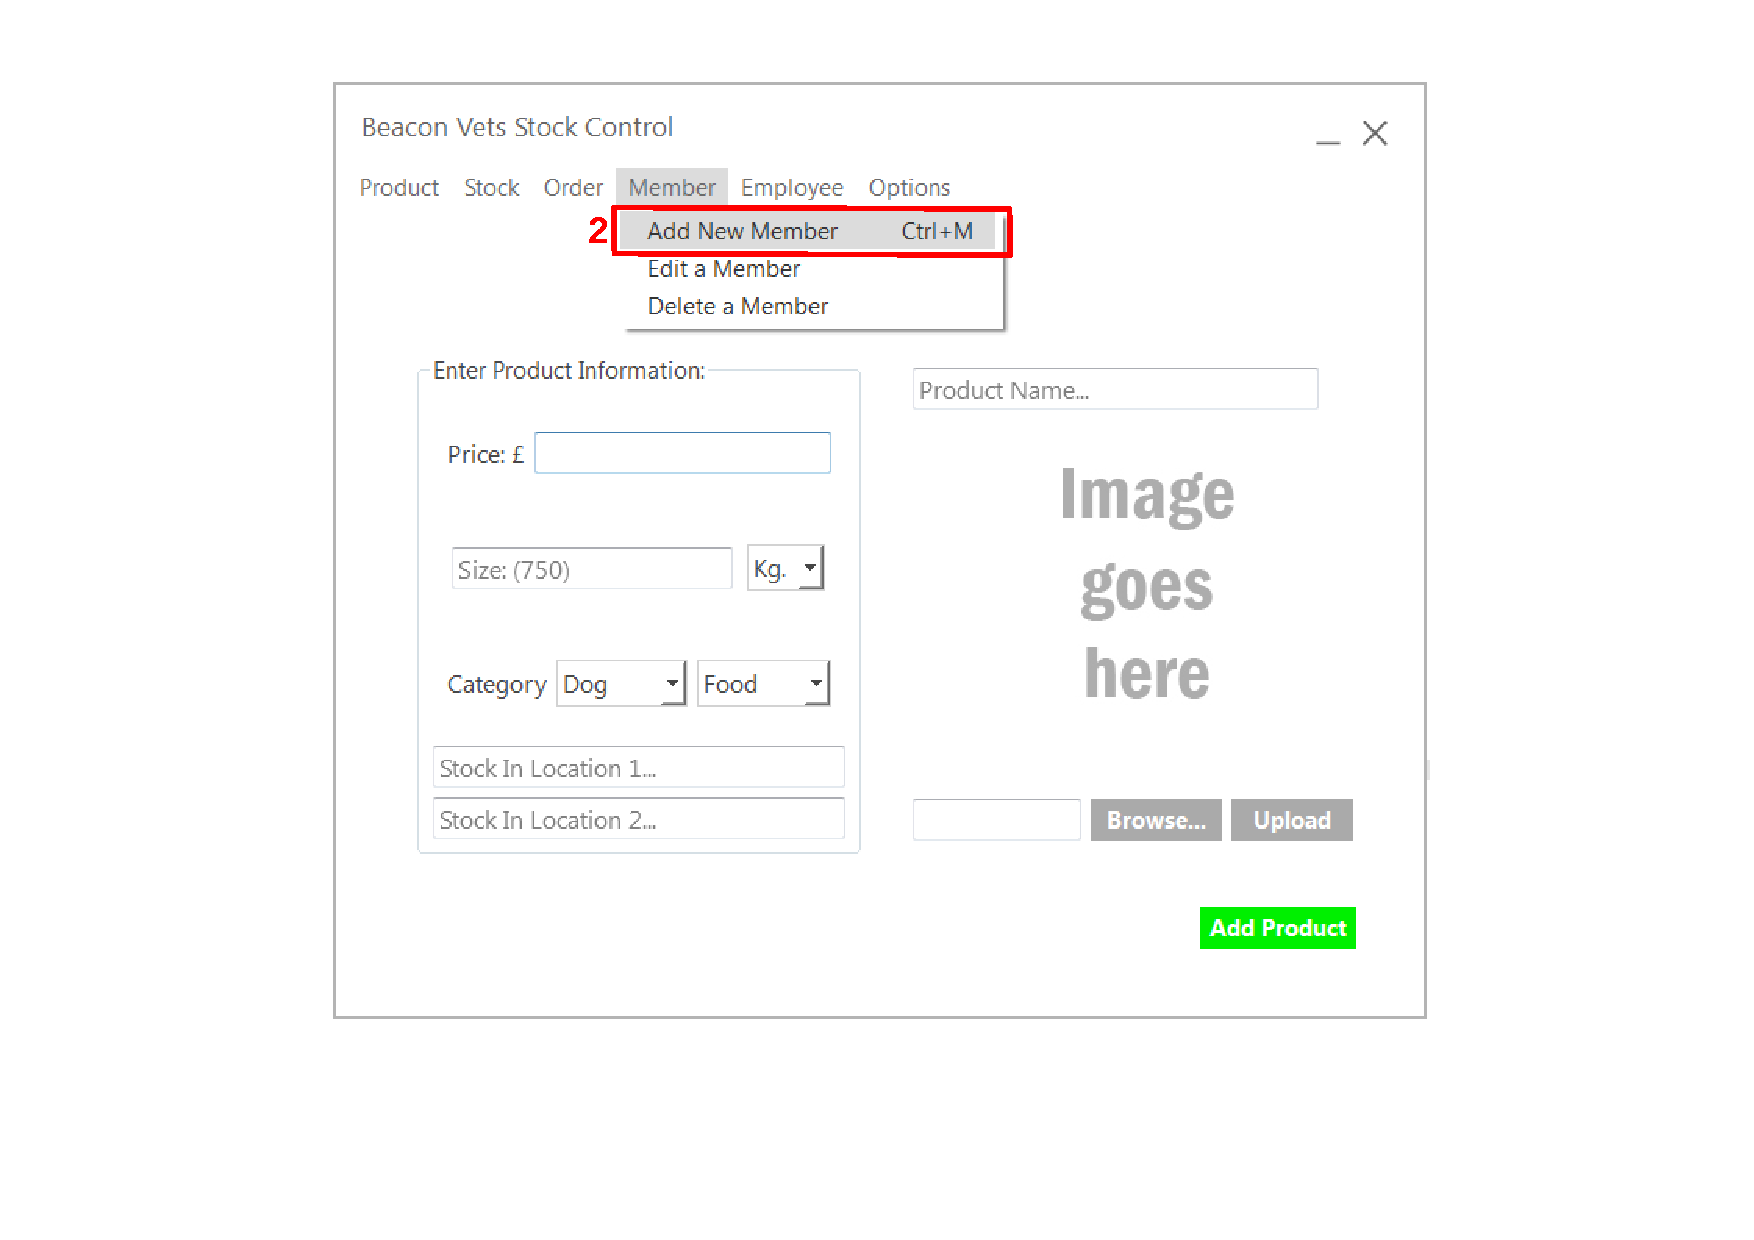
\includegraphics[width=8cm]{./ManualImages/add-member-2.pdf}

An alternative to step 1 and step 2, is by pressing the `CTRL' and `M' button on the keyboard simultaneously.

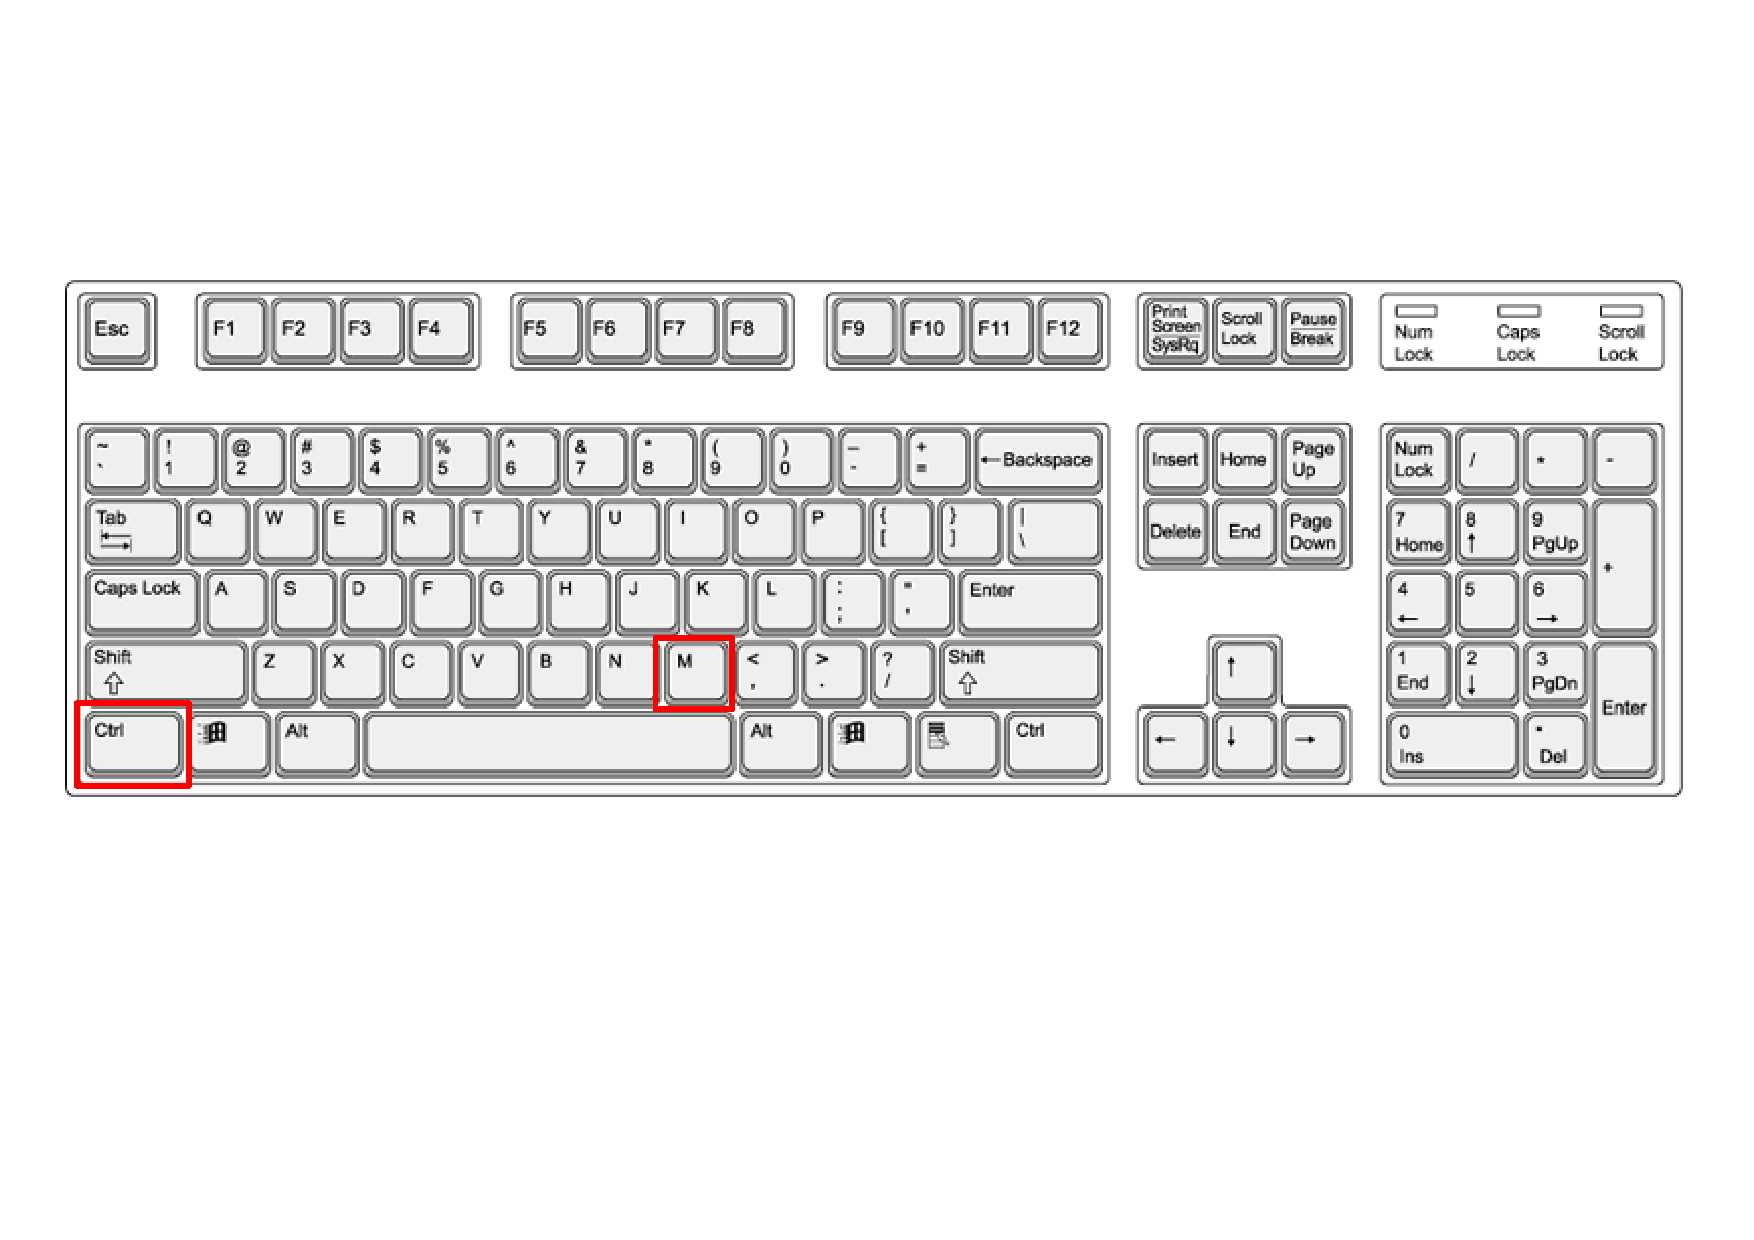
\includegraphics[width=\textwidth]{./ManualImages/shortcut-member.pdf}

\textbf{3.} enter appropriate data into the data fields

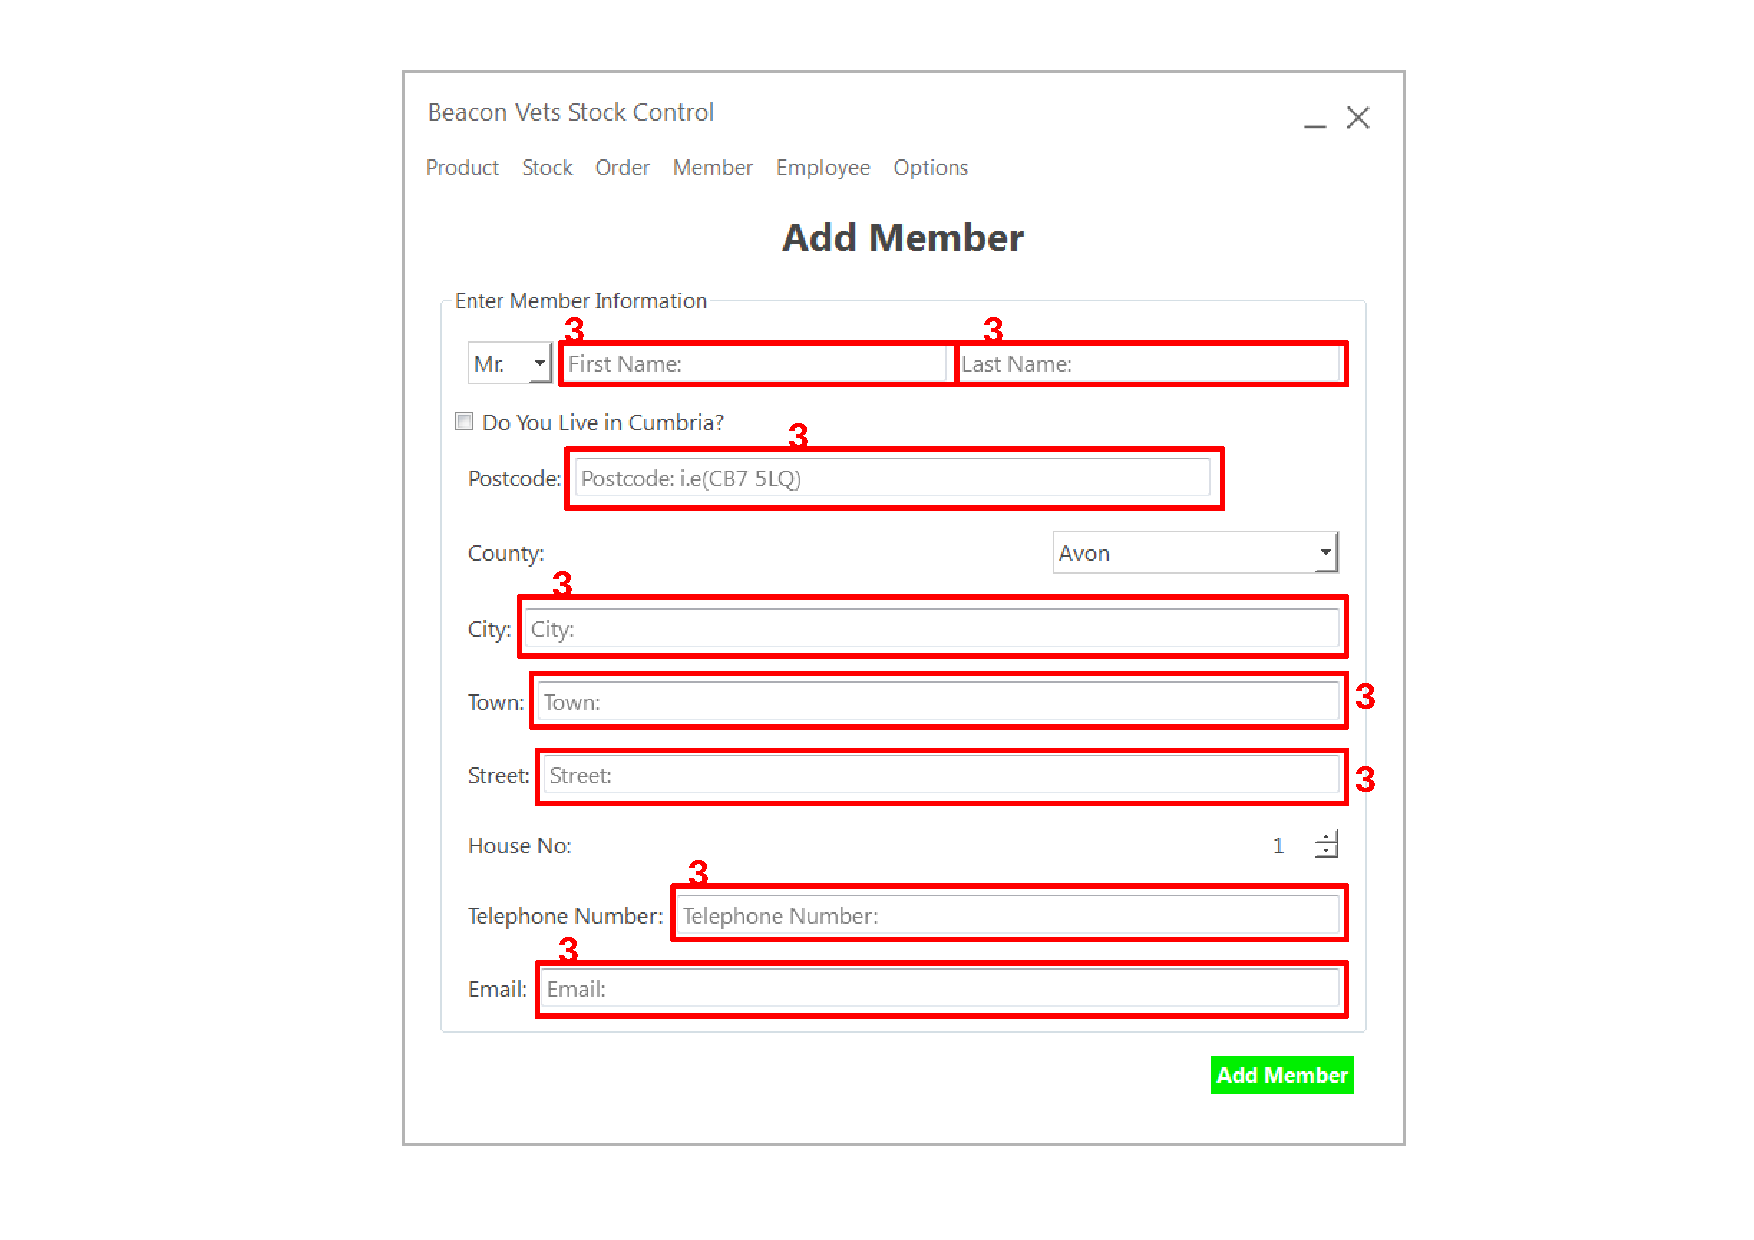
\includegraphics[width=8cm]{./ManualImages/add-member-3.pdf}

\textbf{4.} choose an appropriate option from the drop down menus

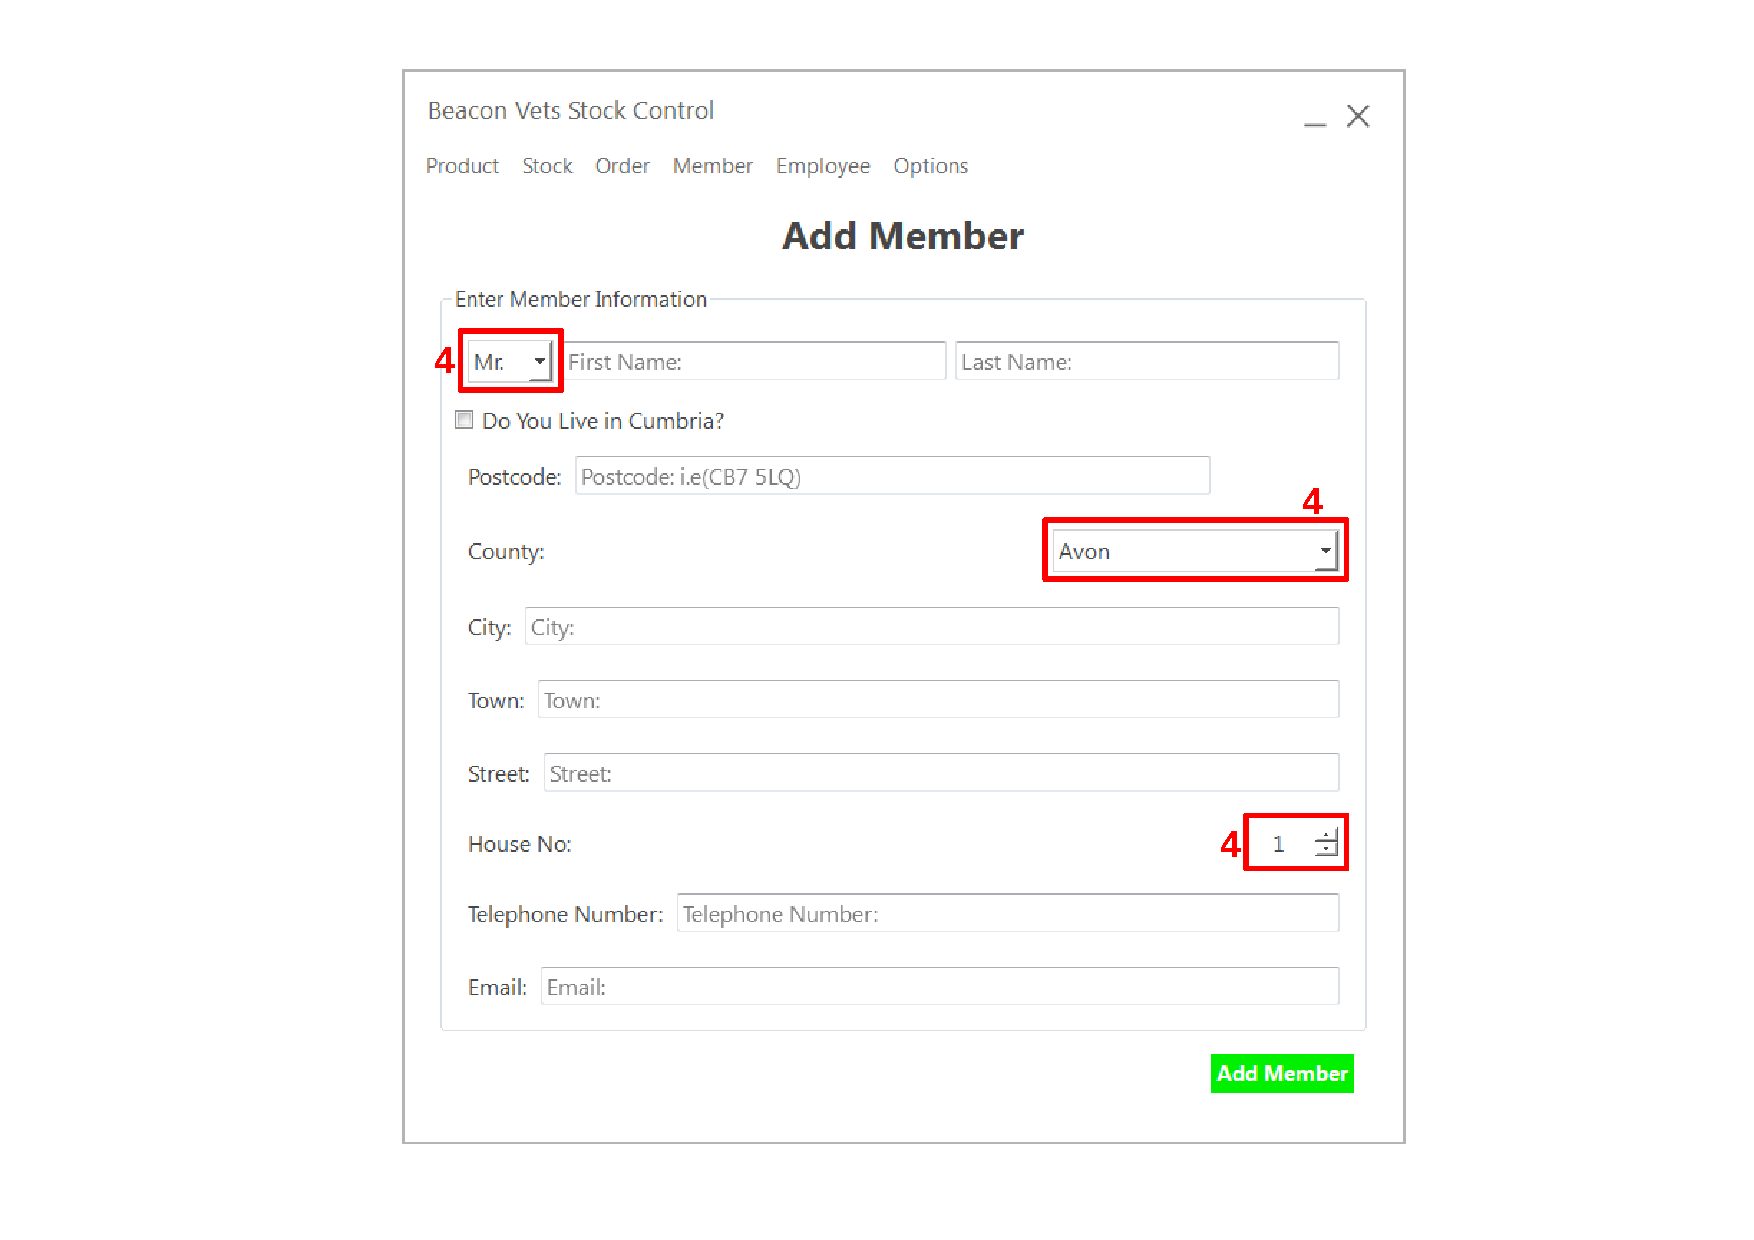
\includegraphics[width=8cm]{./ManualImages/add-member-4.pdf}

if the postcode entered is located within Cumbria, go to step 5, otherwise, go to step 7 .

\textbf{5.} check the tick-box, a button will appear.

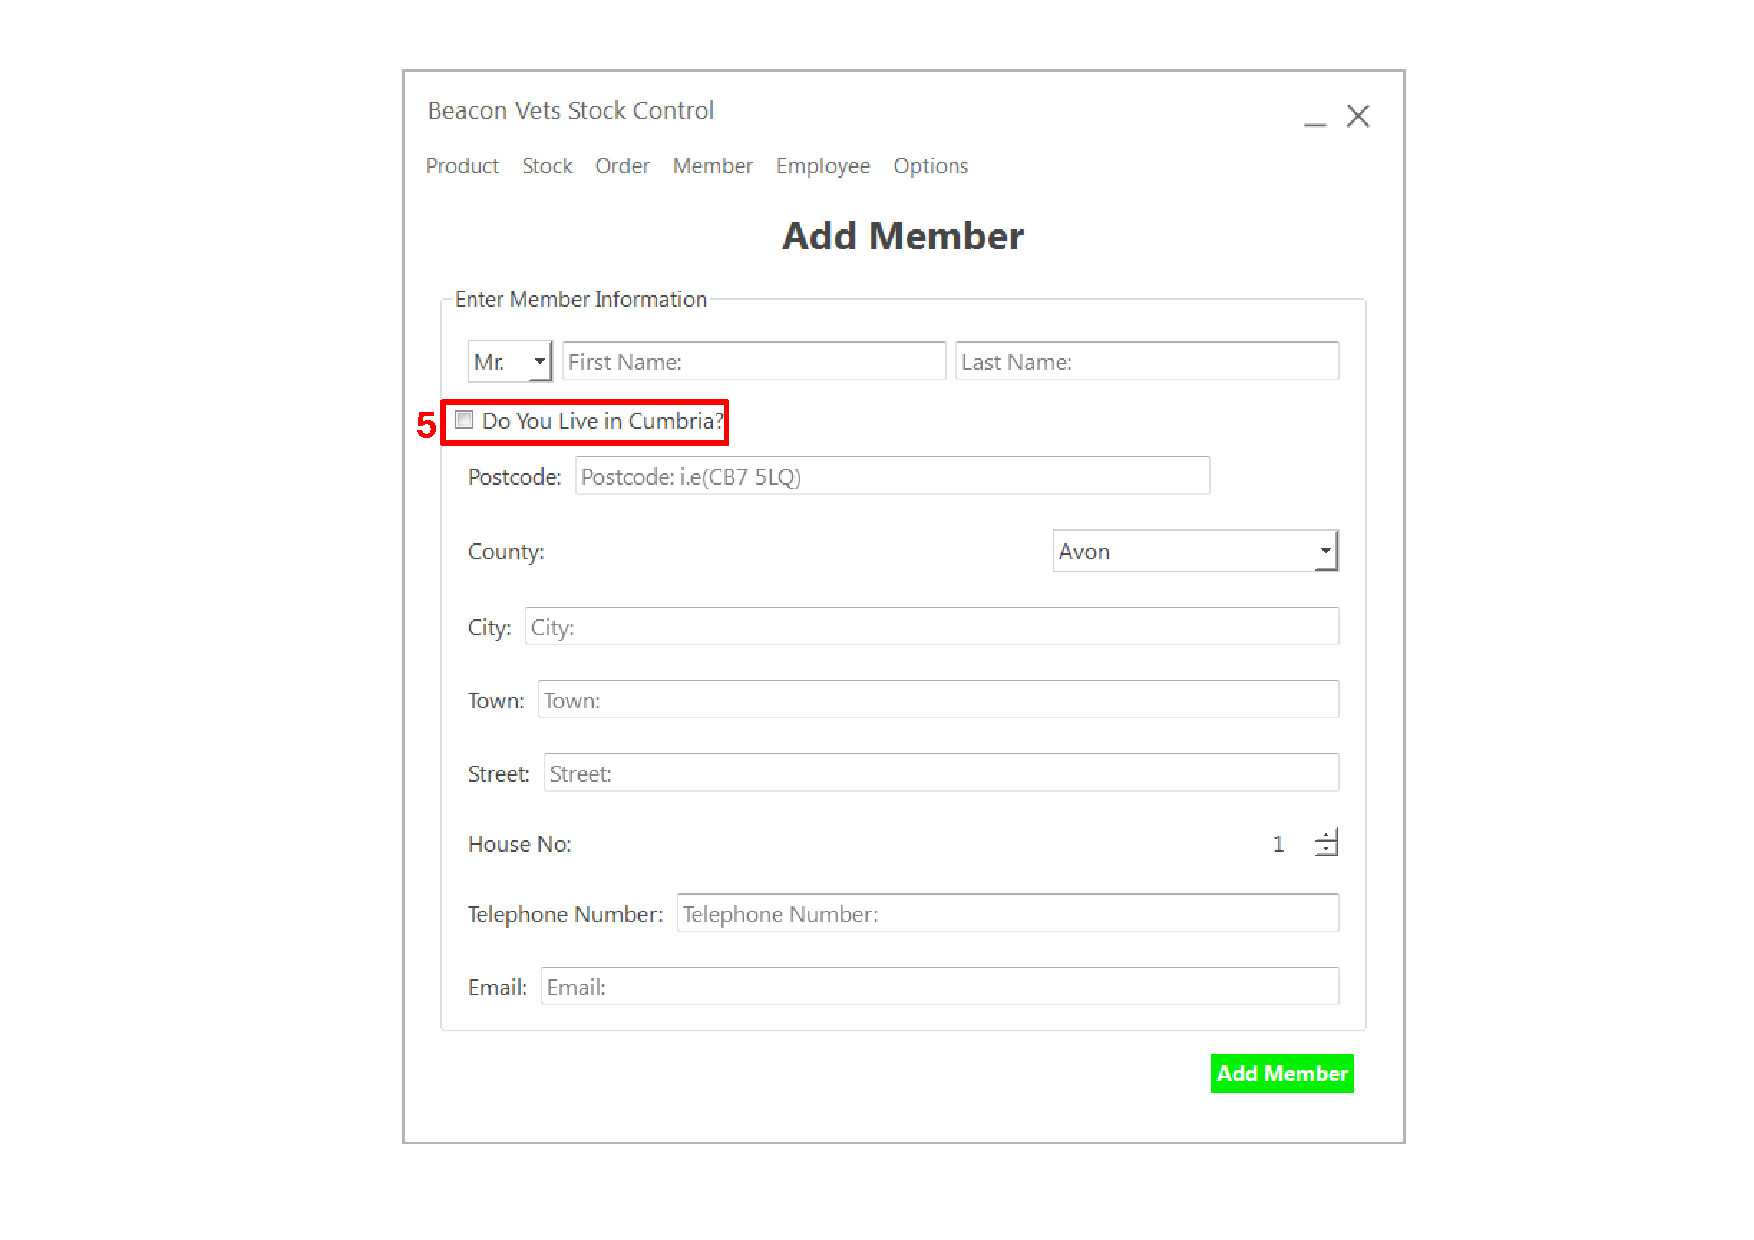
\includegraphics[width=8cm]{./ManualImages/add-member-5.pdf}

\textbf{6.} click the find button once a postcode has been entered, this should cause some of the data fields to be automatically completed.

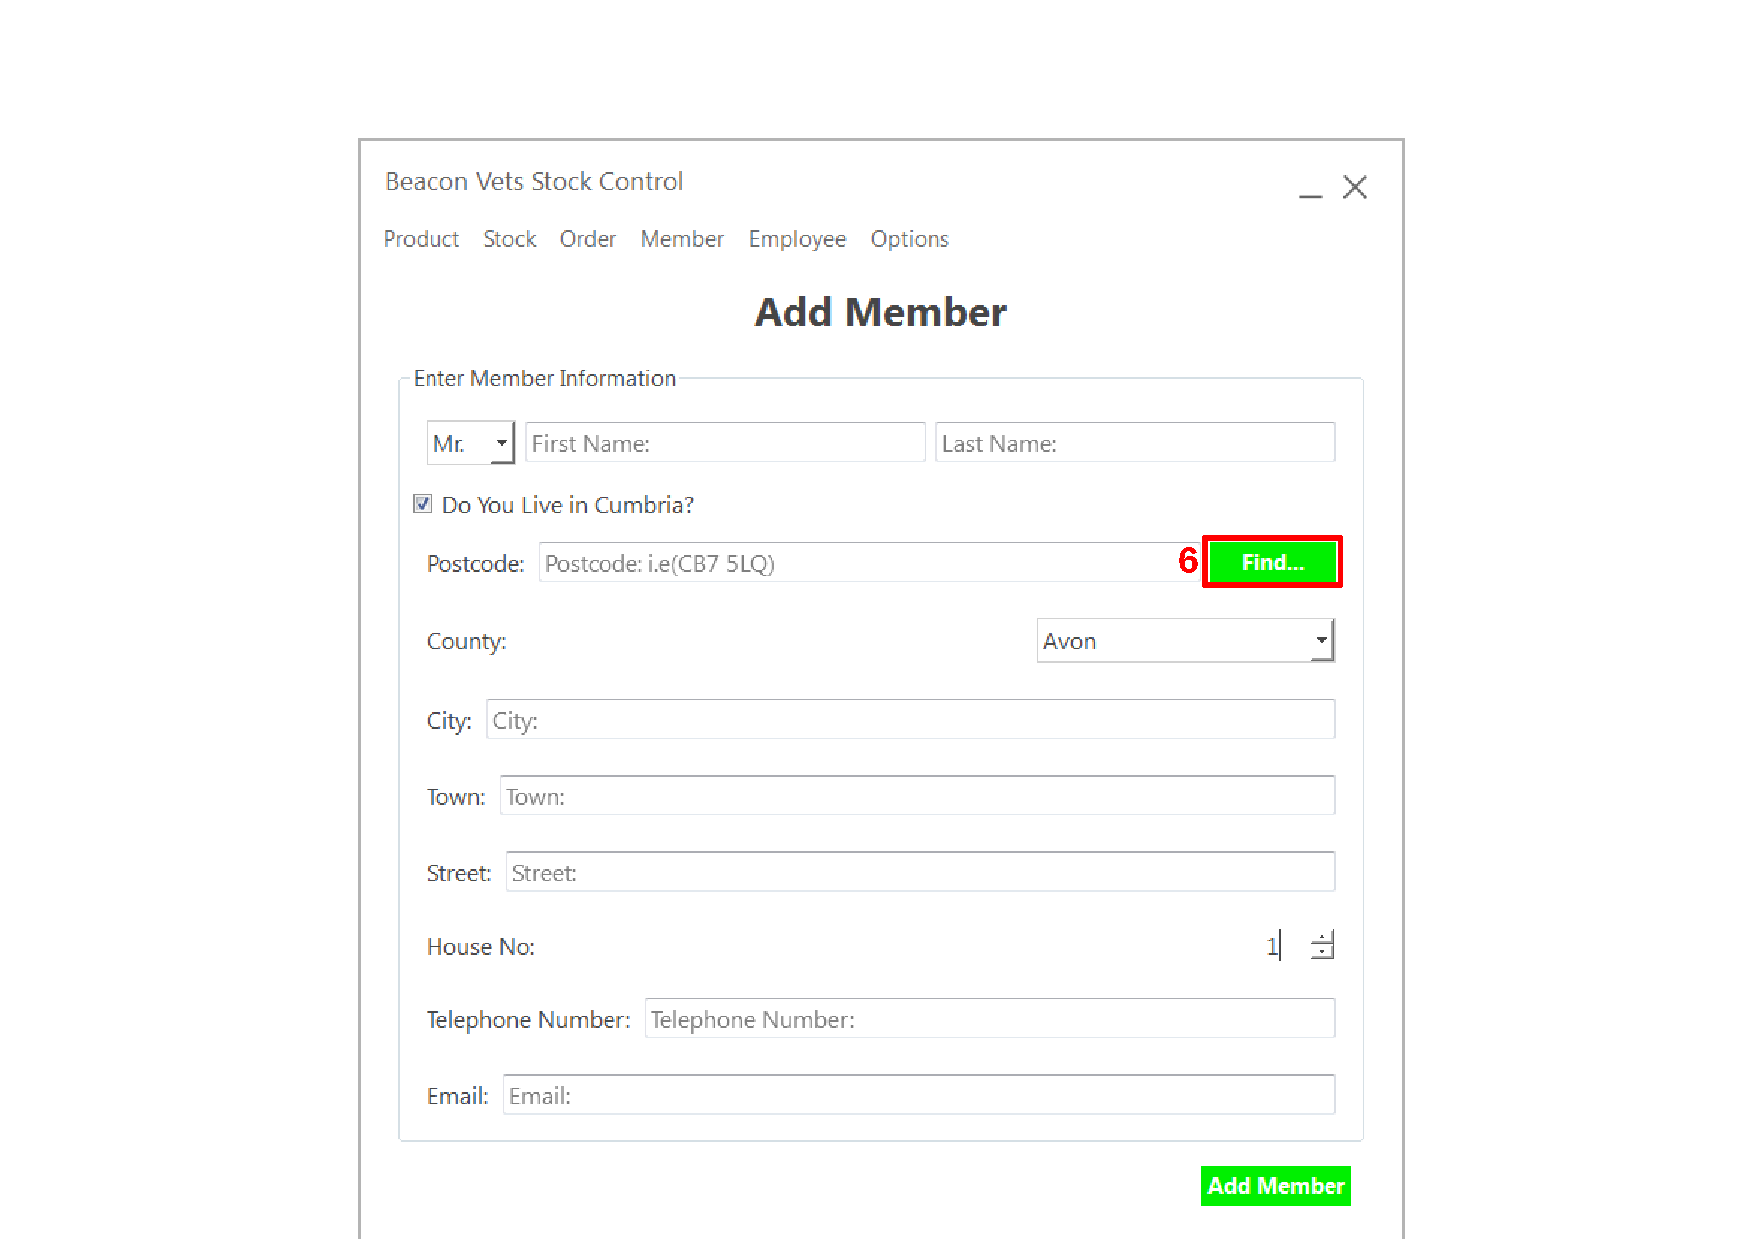
\includegraphics[width=8cm]{./ManualImages/add-member-6.pdf}

\textbf{7.} click the `Add Member' button.

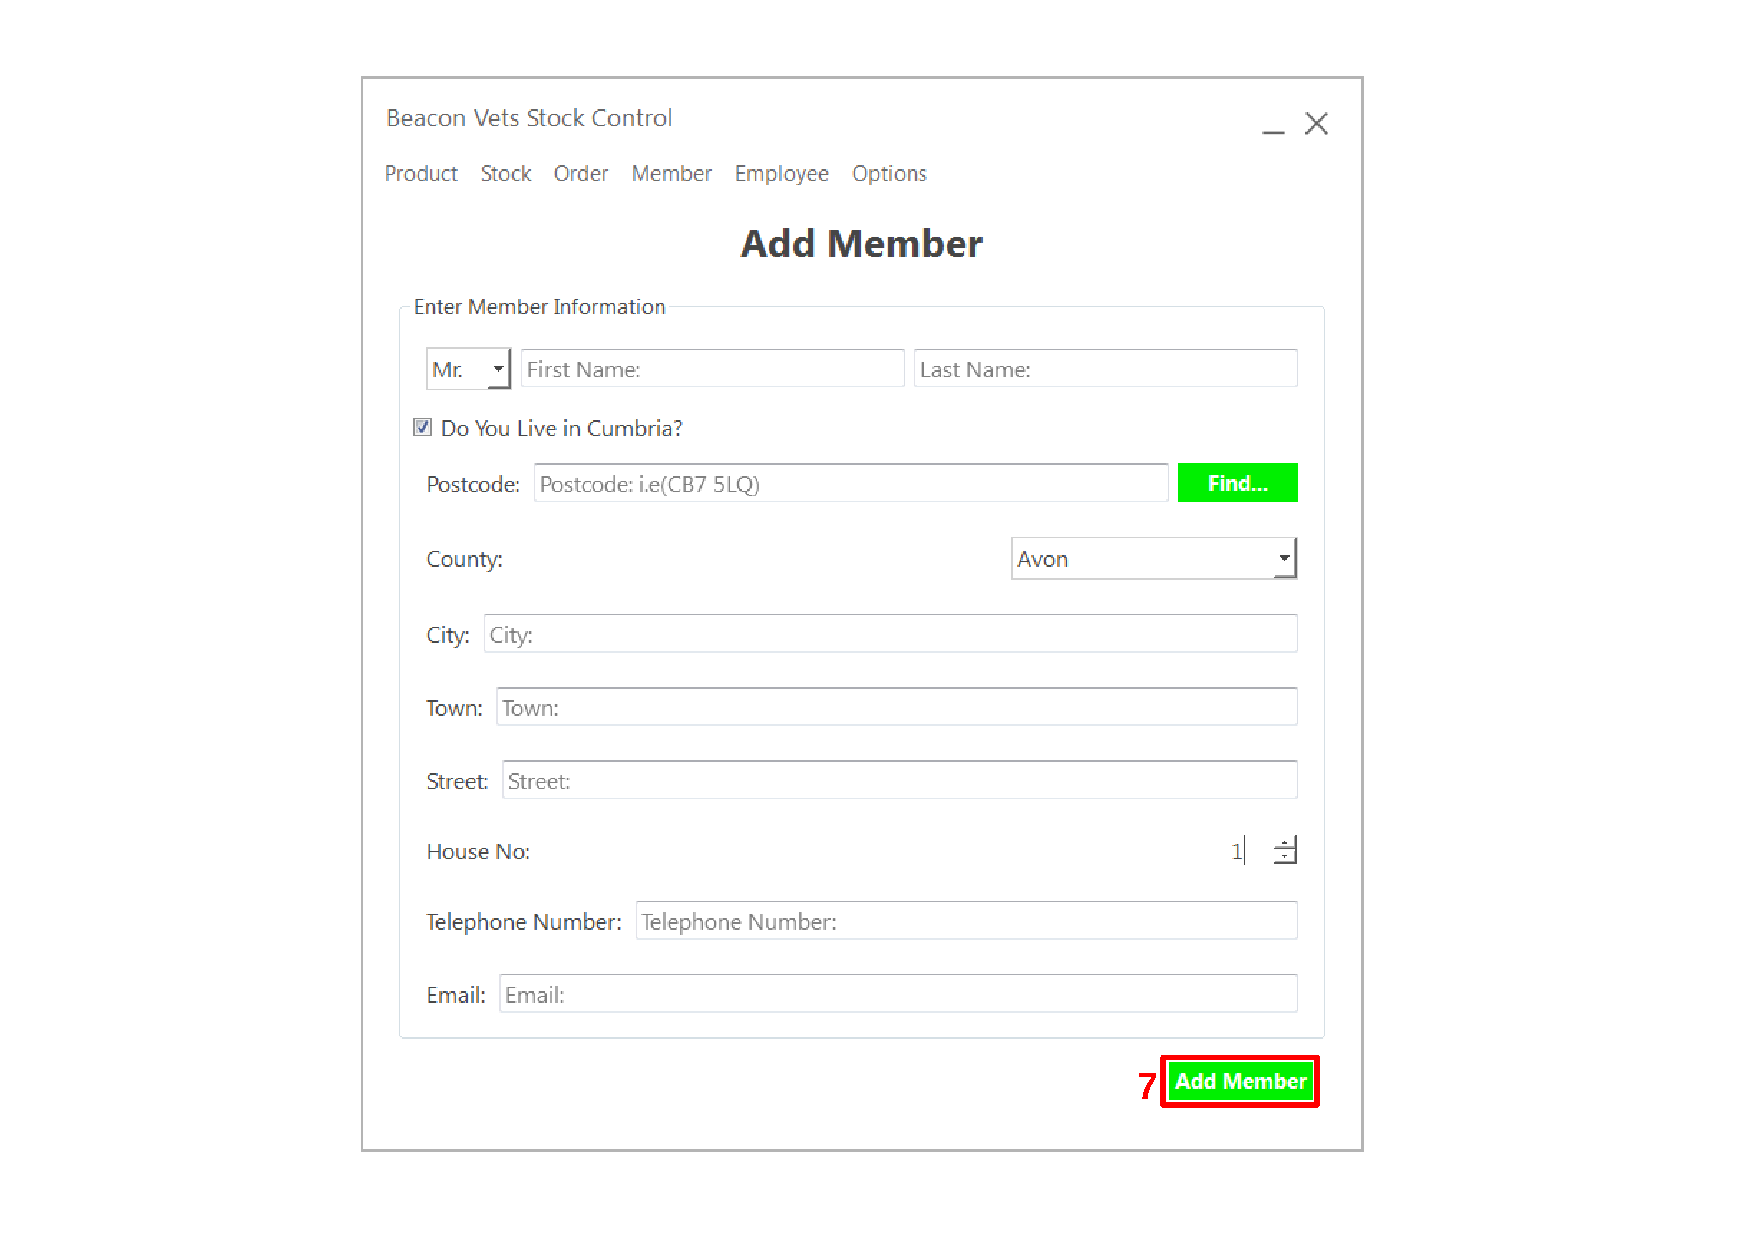
\includegraphics[width=8cm]{./ManualImages/add-member-7.pdf}

\textbf{8.} Click on the `Yes' button on the pop up window

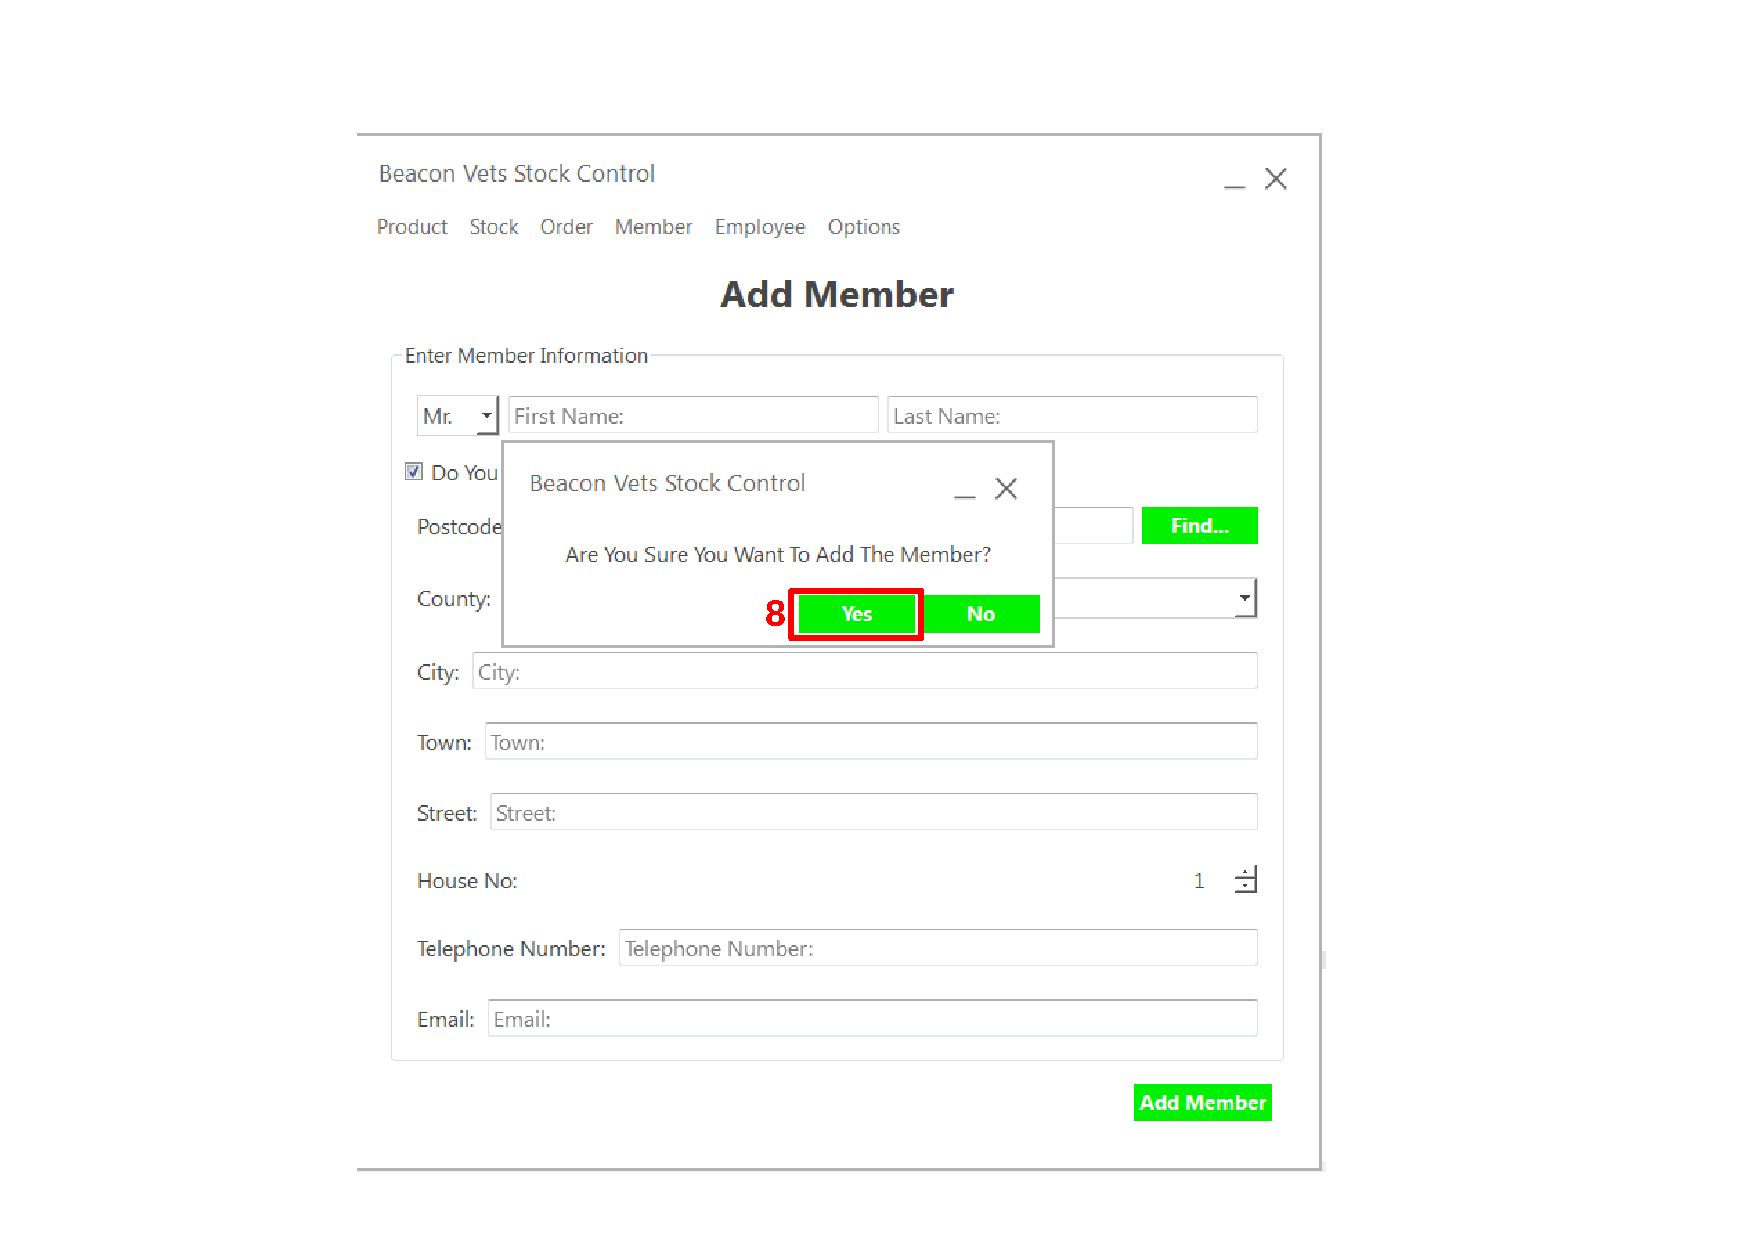
\includegraphics[width=8cm]{./ManualImages/add-member-8.pdf}

\textbf{9.} Click on the `Ok' button on the pop up window

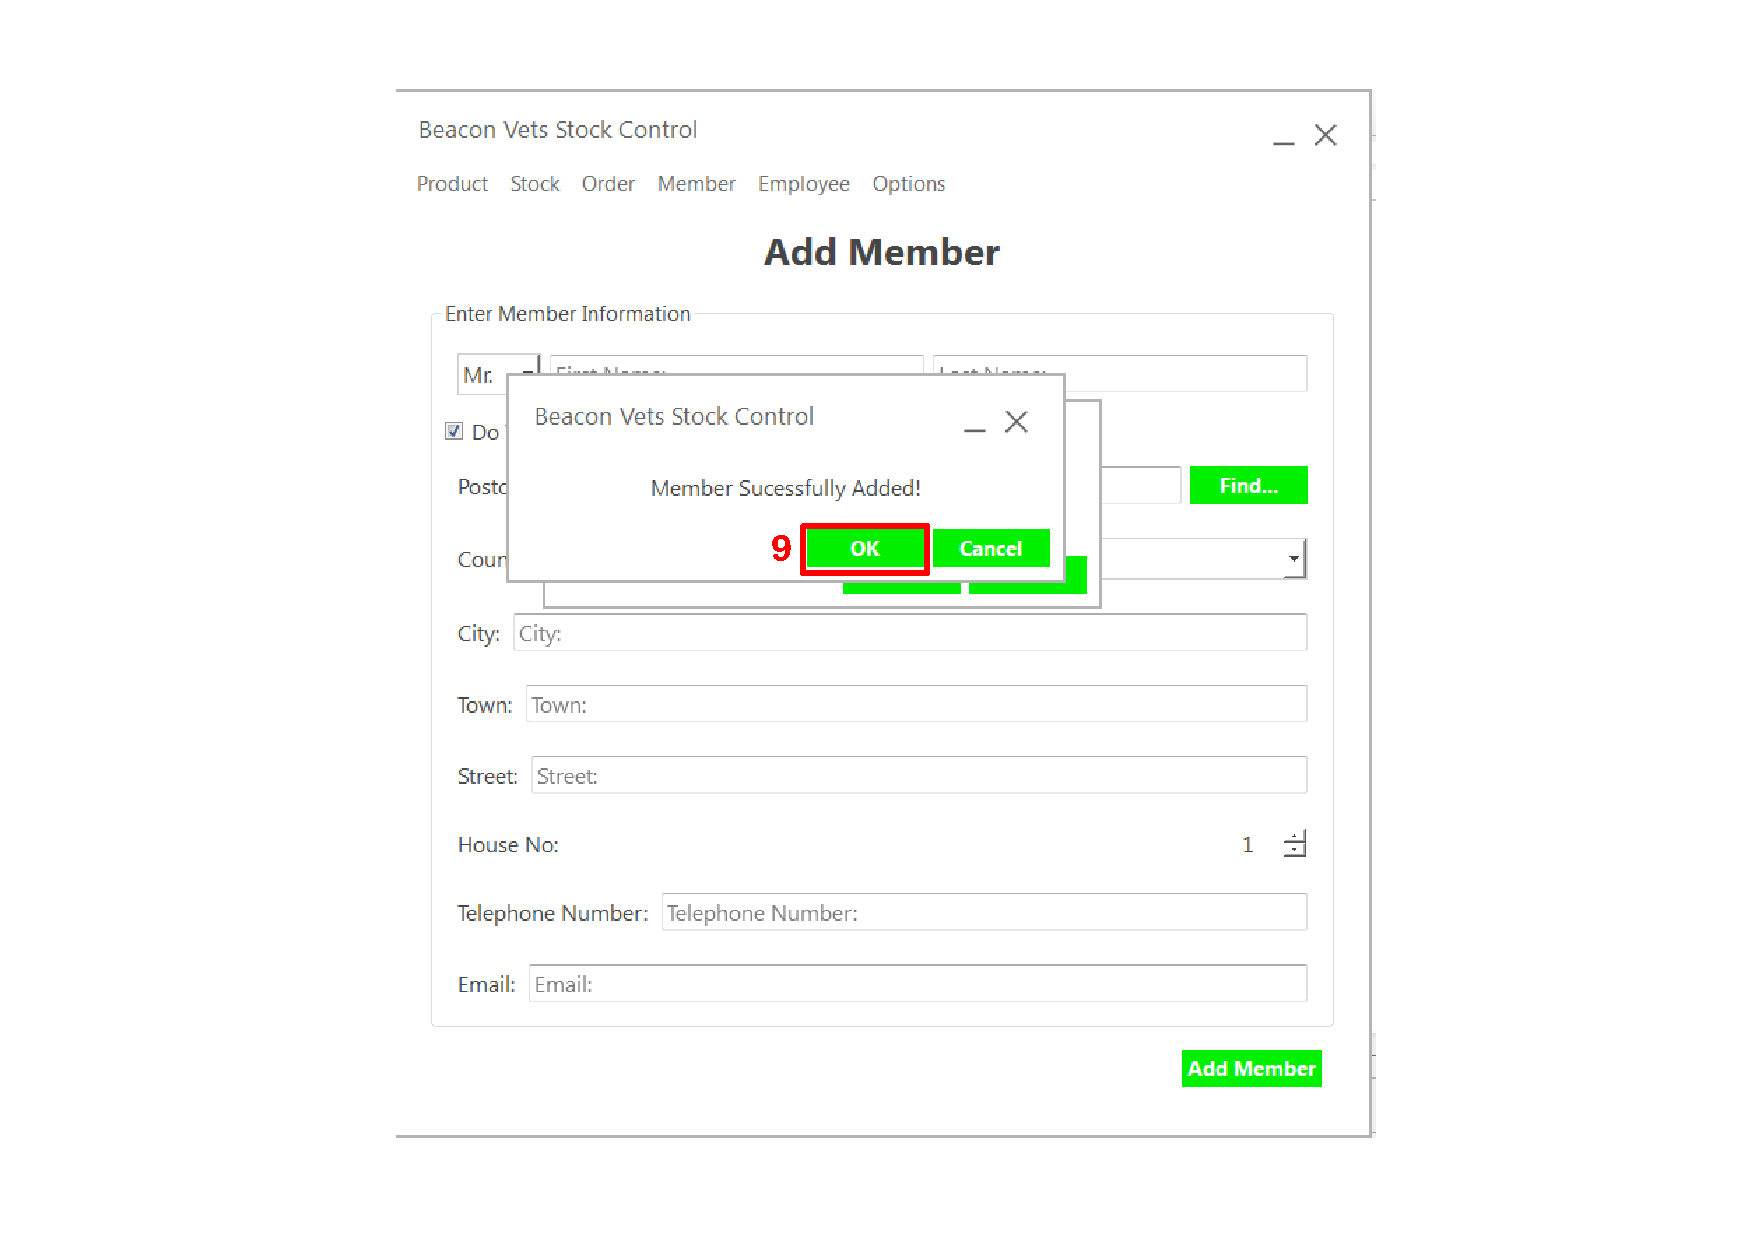
\includegraphics[width=8cm]{./ManualImages/add-member-9.pdf}

You have now successfully added a Member to the system.

\pagebreak
\subsubsection{Adding an Employee to the system}
\label{fig:Adding an Employee to the system}

\textbf{1.} On any interface, click on the `Employee' option within the menu bar.

\textbf{2.} Click on the `Add an Employee' option from the drop down menu.

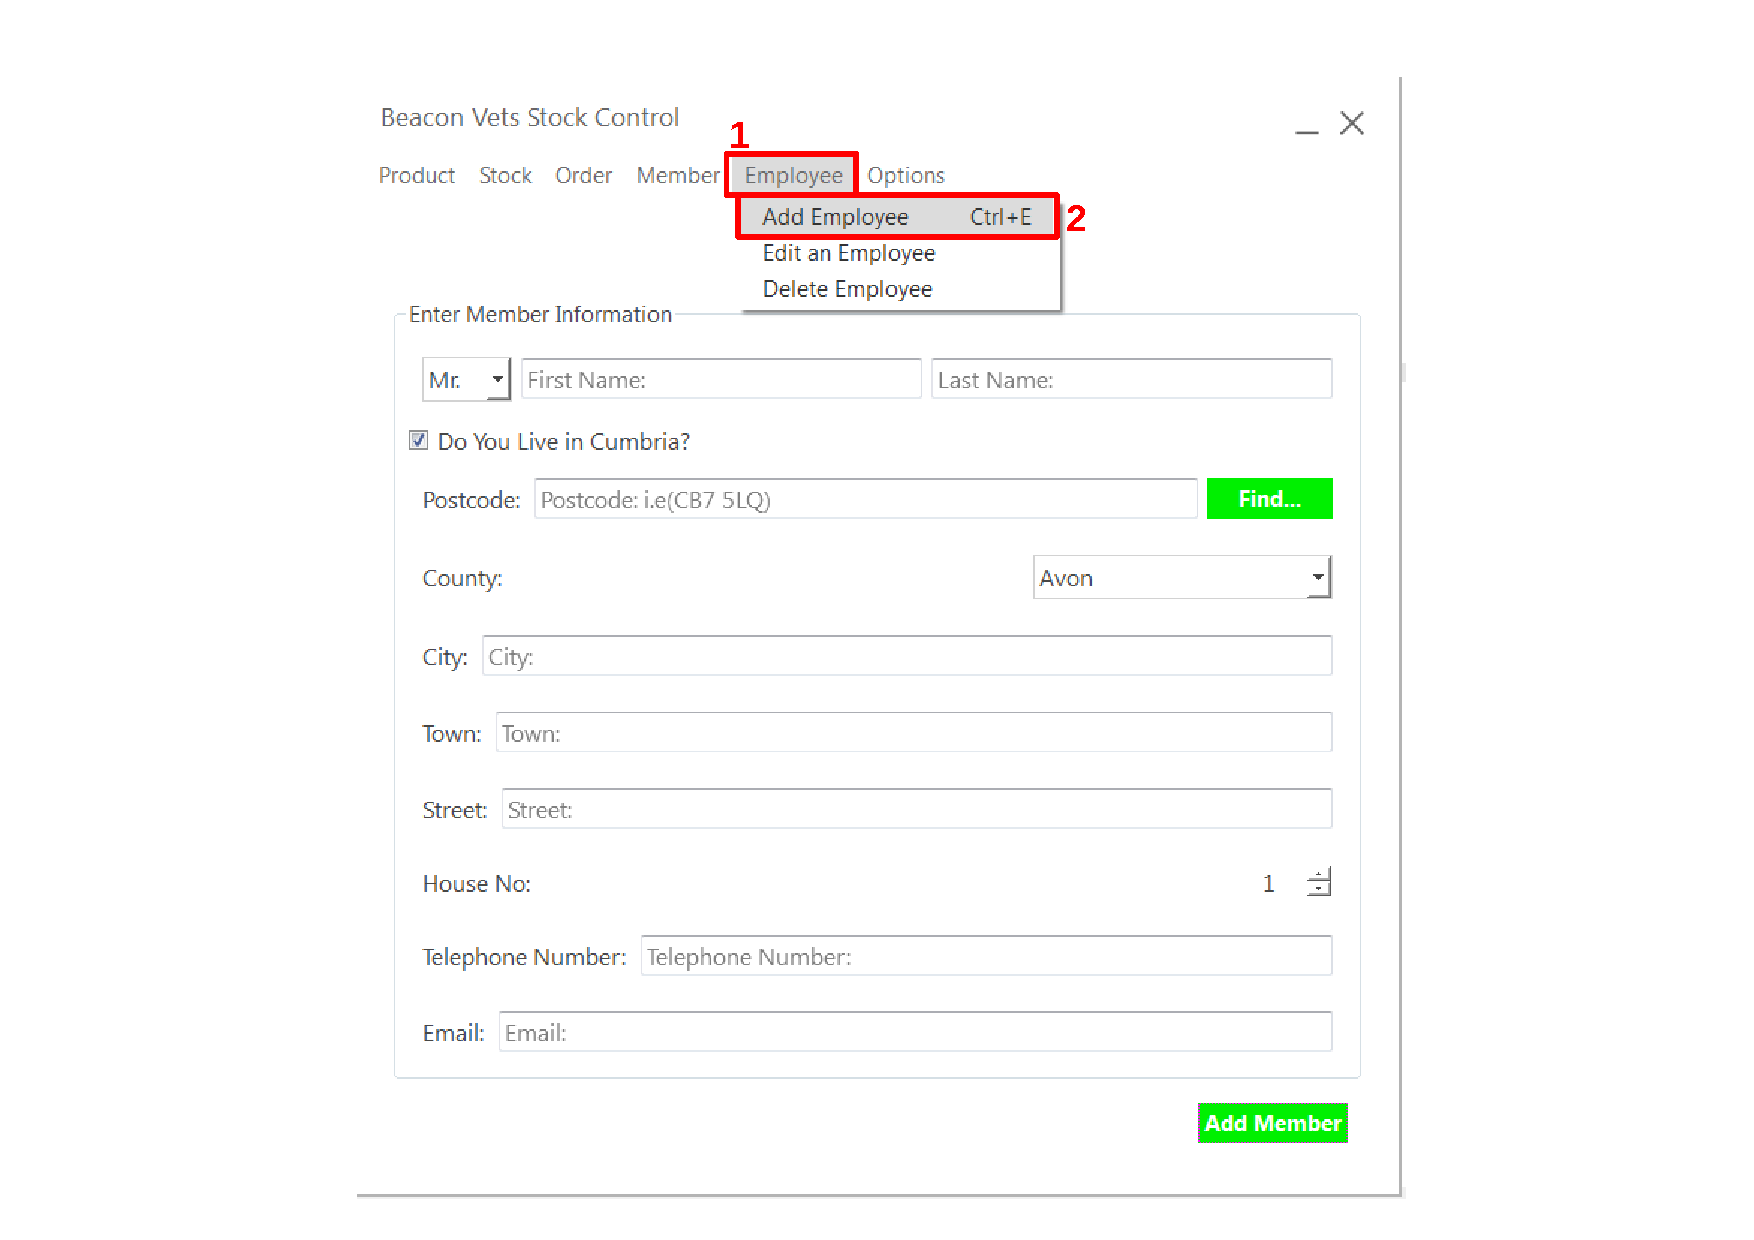
\includegraphics[width=8cm]{./ManualImages/add-employee-1.pdf}

An alternative to step 1 and step 2, is by pressing the `CTRL' and `E' button on the keyboard simultaneously.

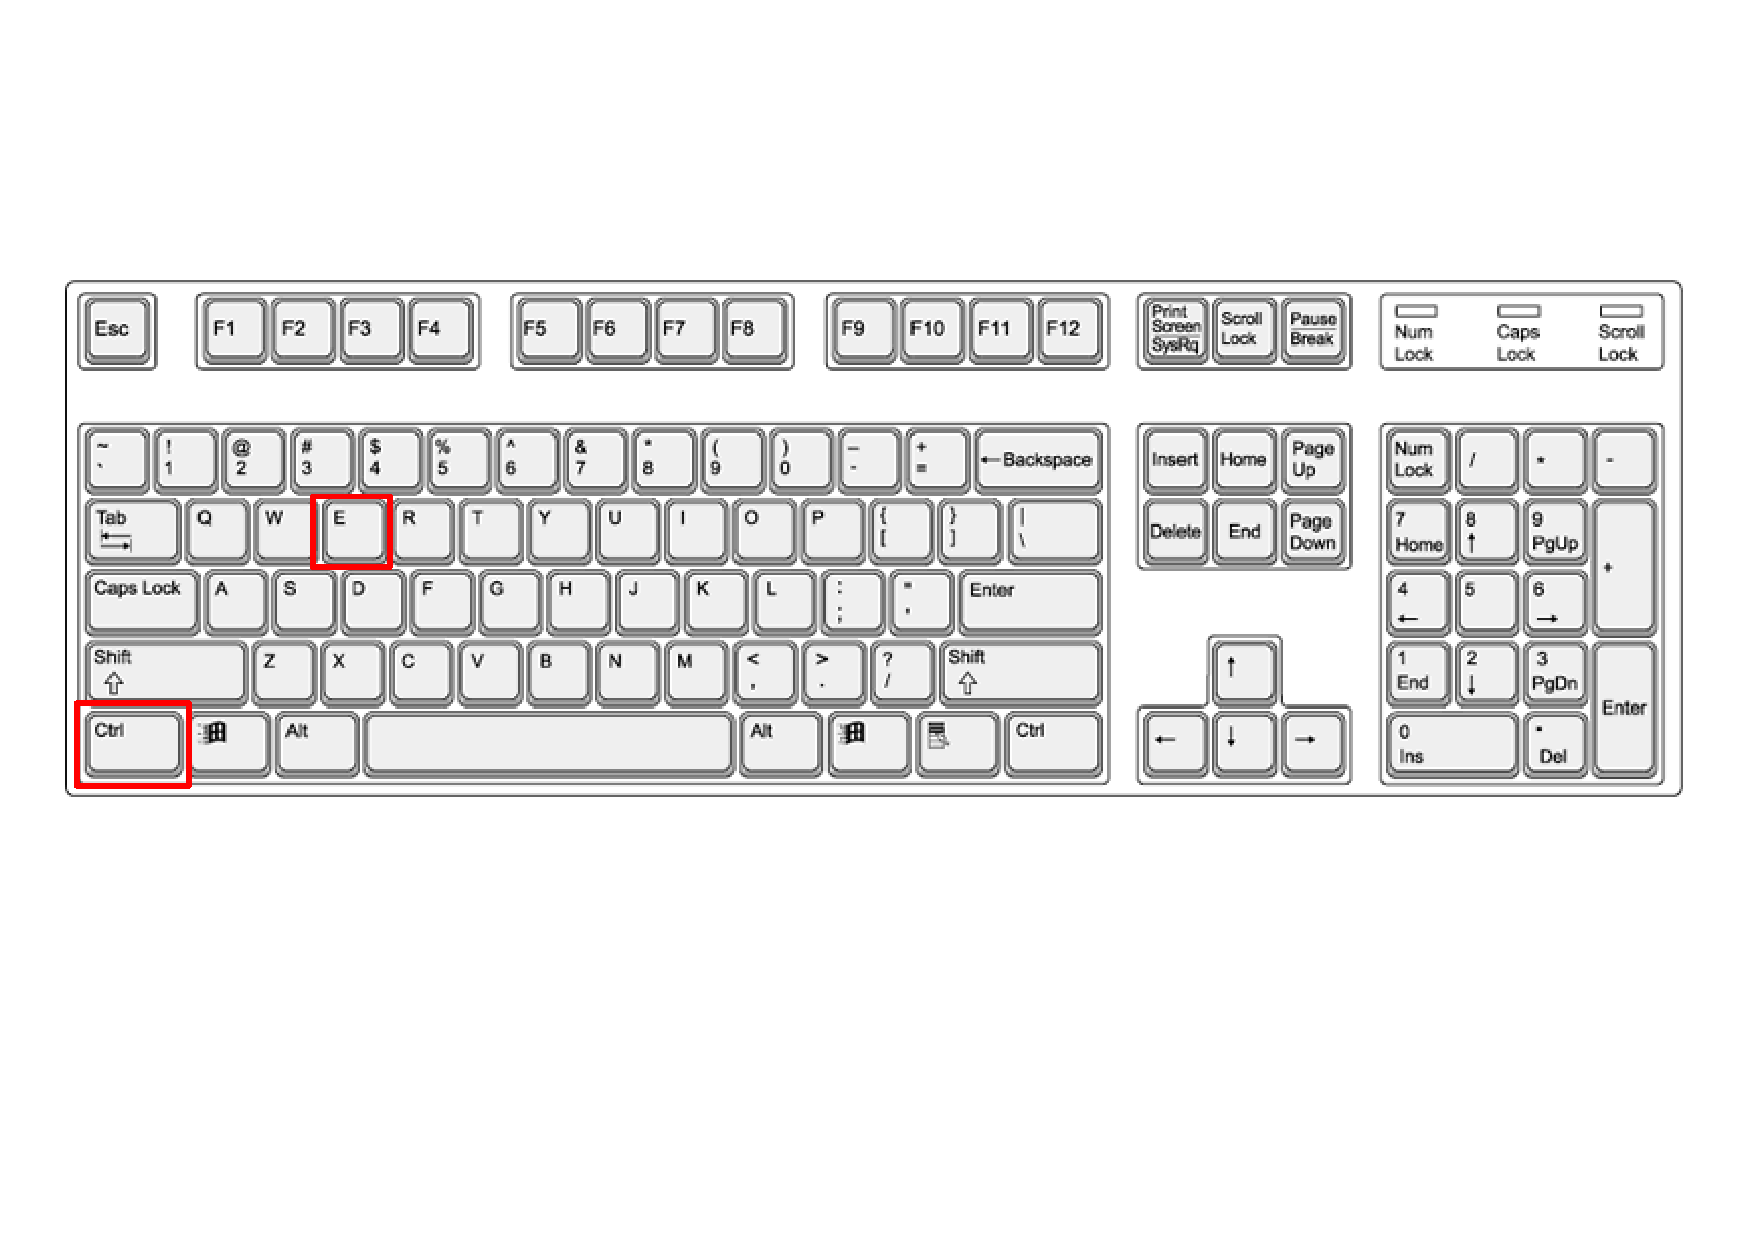
\includegraphics[width=\textwidth]{./ManualImages/shortcut-employee.pdf}

\pagebreak
\subsubsection{Editing a Product in the system}
\label{fig:Editing a Product in the system}


\pagebreak
\subsubsection{Editing a Member currently in the system}
\label{fig:Editing a Member currently in the system}


\pagebreak
\subsubsection{Editing an Employee in the system}
\label{fig:Editing an Employee in the system}


\pagebreak
\subsubsection{Removing a Product from the system}
\label{fig:Removing a Product from the system}


\pagebreak
\subsubsection{Removing a Member from the system}
\label{fig:Removing a Member from the system}


\pagebreak
\subsubsection{Removing an Employee for the system.}
\label{fig:Removing an Employee for the system.}


\pagebreak
\subsubsection{Finding a Product within the system}
\label{fig:Finding a Product within the system}


\pagebreak
\subsubsection{Finding a Member in the system}
\label{fig:Finding a Member in the system}


\pagebreak
\subsubsection{Finding an Employee in the system}
\label{fig:Finding an Employee in the system}


\pagebreak
\subsubsection{Changing the stock of a Product}
\label{fig:Changing the stock of a Product}


\pagebreak
\subsubsection{Product Stock Prediction}
\label{fig:Product Stock Prediction}


\pagebreak
\subsubsection{Creating an Order}
\label{fig:Creating an Order}


\pagebreak
\subsubsection{Adding products to an order}
\label{fig:Adding products to an order}


\pagebreak
\subsubsection{Applying a Discount to an Order}
\label{fig:Applying a Discount to an Order}


\pagebreak
\subsubsection{Previewing the invoice}
\label{fig:Previewing the invoice}


\pagebreak
\subsubsection{Printing an invoice}
\label{fig:Printing an invoice}


\pagebreak
\subsubsection{Emailing an invoice}
\label{fig:Emailing an invoice}


\pagebreak
\subsubsection{Changing information on the invoice}
\label{fig:Changing information on the invoice}


\pagebreak
\subsubsection{Problems with sending emails}
\label{fig:Problems with sending emails}


\pagebreak
\subsubsection{Changing your Password}
\label{fig:Changing your Password}


\pagebreak
\subsubsection{Accessing the search window}
\label{fig:Accessing the search window}




\subsection{Saving}

\subsection{Limitations}

\section{Error Recovery}

%include as many subsections as necessary for each error
\subsection{Error 1}

\subsection{Error 2}

\section{System Recovery}

\subsection{Backing-up Data}

\subsection{Restoring Data}